\documentclass[10pt, letterpaper]{report}
% !TeX program = xelatex
%==================PREAMBOLO=======================%
\input{../../preamble/preamble.tex}
\newcommand{\titolo}{Robotics 1 }

 %TOGLI COMMENTO SE USI XELATEX
%\usepackage{fontspec}
\title{\titolo} %========TITOLO========%
\author{Marco Casu}
\date{\vspace{-5ex}}
\begin{document}

%==================COPERTINA=======================%
\begin{titlepage}
    
\begin{center}
    %TOGLI COMMENTO SE USI XELATEX
   %\setmainfont{Palace Script MT}
   \HUGE Marco Casu\acc
\end{center}
\thispagestyle{empty}
\begin{figure}[h]
    \centering{
        %l'immagine deve avere una risoluzione 2048x2048
        \includegraphics[width=1\textwidth ]{images/Copertina.png}
    }
\end{figure}
\vfill 
\centering \includegraphics[width=0.4\textwidth ]{../../preamble/Stemma_sapienza.png} \acc
\centering \Large \color{sapienza}Faculty of Information Engineering, Computer Science and Statistics\\
Department of Computer, Control and Management Engineering\\
Master's degree in Artificial Intelligence and Robotics
\end{titlepage}

%===================FINE COPERTINA======================%
\newpage
%\pagecolor{cartaRiciclata}%\setmainfont{Algerian}
\Large
This document summarizes and presents the topics for the \titolo course for the Master's degree in Artificial Intelligence and Robotics at Sapienza University of Rome. The document is free for any use. If the reader notices any typos, they are kindly requested to report them to the author.
\vfill
\begin{figure}[h!]
    \raggedright
    \includegraphics[width=0.4\textwidth,right ]{../../preamble/tomodachi.pdf} 
\end{figure}
\newpage %\setmainfont{Times New Roman}
\normalsize

\tableofcontents 
\newpage

%==================FOOTER e HEADER=======================%
\fancyhf{}
\fancyhead[L]{\nouppercase{\leftmark}}
\fancyhead[R]{Sezione \thesection}
\fancyfoot[C]{\thepage}
\fancyfoot[L]{\titolo}
\fancyfoot[R]{ Marco Casu}
%\fancyfoot[R]{\setmainfont{Palace Script MT}\huge Marco Casu \setmainfont{Times New Roman}}
%==================FOOTER e HEADER=======================%
\newtheorem{definition}{Definition}
\newtheorem{proposition}{Proposition}
\newtheorem{theorem}{Theorem}
%==================INIZIO======================%
\chapter{Introduction}
In this chapter we will see a brief introduction to the mathematical tools used in the main topics of the course. The topics presented in this section may seem somewhat unclear, as many concepts and definitions are only briefly introduced and deliberately not elaborated upon. They will be discussed in detail in their respective chapters.\bigskip
\section{About the End Effector Pose}
A robot is made up of a series of arms connected to one another by joints, these joints can be \textbf{revolut} or \textbf{prismatic} (as shown in figure \ref{img:joints}), a revolut joint rotate the link connected along 1 axis, the prismatic joint can make the link extend or contract, making them translate along 1 axis.

\begin{figure}[h!]
    \centering
    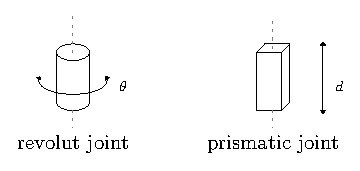
\includegraphics[width=0.6\textwidth ]{images/joints.eps} 
    \caption{two types of joints (spatial representation)}
    \label{img:joints}
\end{figure}

It is important to know that that if the angle $\theta$ increase the joint is rotating counter clock wise. In a planar drawing, the joints are denoted as shown in image \ref{img:joints_planar}.

\begin{figure}[h!]
    \centering
    \includegraphics[width=0.6\textwidth ]{images/joints_planar.eps} 
    \caption{planar representation of the joints}
    \label{img:joints_planar}
\end{figure}

In the mathematical/geometrical model of a robotic arms, it is important the \textit{kinematic skeleton}, the quantities involved are\begin{itemize}
    \item the current angle of the joints
    \item the length of the links
\end{itemize}
everything is defined respect to the base frame, usually denoted as $\Sigma_0$.

\begin{figure}[h!]
    \centering
    \includegraphics[width=0.45\textwidth ]{images/spatial_robot_new.eps} 
    \caption{spatial R4 robot}
    \label{img:spatialR4}
\end{figure}
\bigskip

The robot shown in figure \ref{img:spatialR4} is an \textit{R4 robot} (4 revolut joints) with three links. With ${}^0\mathbf p_e$ and $\Sigma_e$ we denote the position and the reference frame of the \textbf{end effector}, if there are a 0 supscript to a vector, we mean that is expressed in the base reference frame.\bigskip

With \textbf{Direct Kinematics}, we define the problem to find what are the \textbf{pose} (position and orientation) of the end effector, in function of the joint's angles. \begin{align}
    &Kin_p(\boldsymbol{\theta}):\Sigma_0\rightarrow\Sigma_e\\
    &\boldsymbol{\theta}=\begin{pmatrix}
        \theta_1&\theta_2&\theta_3&\theta_4
    \end{pmatrix}^T
\end{align}
With $\Sigma_e$ is denoted the reference frame of the end effector. How can we compute $Kin_p(\boldsymbol{\theta})$? This is given by an homogeneous $4\times 4$ matrix defined as follows:\begin{equation}
    {}^0T_e=\begin{pmatrix}
        & & & \\
        & {}^0R_e & &{}^0\mathbf p_e \\
        & & & \\
        0& 0&0 &1 
    \end{pmatrix}
\end{equation}
where\begin{itemize}
    \item ${}^0R_e\in SO(3)$ is the rotation matrix, and depends from $\boldsymbol{\theta}$
    \item ${}^0\mathbf p_e\in \R^3$ is the translation vector.
\end{itemize}

\noindent\textbf{Recall}: $SO(3)$ is the group of all the orthogonal $3\times 3$ matrices with determinant equals to 1.\bigskip

\noindent The matrix ${}^0T_e$ is obtained by multiplying $n$ matrix (where $n$ is the number of joints)\begin{align}
     &{}^0T_e= {}^0A_1(\theta_1) {}^1A_2(\theta_2)\dots {}^{n-1}A_n(\theta_n)=\\&\prod_{i=0}^{n-1}{}^iA_{i+1}(\theta_{i+1}).
\end{align}
Each \textit{homogeneous matrix} $^{i-1}A_i$ describe the pose of the $i$-th joint's frame respect to the previous joint's frame, and depends from $\theta_i$ (the $i$-th joint's angle). A more detailed description of the matrix describing the direct kinematics will be given later.\bigskip


If there are another frame $\Sigma_w$, the new matrix can be computed as follows\begin{equation}
    {}^w T_e={}^w T_0{}^0 T_e.
\end{equation}\begin{center}
    \includegraphics[width=0.8\textwidth ]{images/T_matrix_new.eps} 
\end{center}

The \textbf{Inverse Kinematics} is the opposite problem, given a position ${}^0\mathbf p_e$ for the end effector, we want to find the values of $\boldsymbol\theta$ such that\begin{equation}
    {}^0\mathbf p_e=Kin_p(\btheta)
\end{equation}
to find $\btheta$, we have to solve a non-linear system of equations, this is generally an undecidable problem, but for some specific cases, there exists a closed form, that can be found analytically, there are also numerical methods. Clearly, for the positions out of the work space, the system does not admit solutions (also this can be checked analytically).
\section{About the End Effector Velocity}
Let's now consider \textbf{Differential Kinematics}, that is the problem to find the end effector velocity in the workspace given the velocity of the joint's angles. 
Since the superposition principle is valid, the components resulting from the movement of each individual joint, which constitute the final velocity of the end effector, can be considered separately. It is important to know that the velocity component of the end effector given by a joint, is always orthogonal to the rotation axis of that joint.\bigskip

\noindent The end effector have\begin{itemize}
    \item a linear velocity, usually denoted $\mathbf v$
    \item an angular velocity, usually denoted $\bomega$.
\end{itemize}
\begin{figure}[h!]
    \centering
    \includegraphics[width=0.28\textwidth ]{images/velocity_new.eps} 
    \caption{possible trajectory by moving $\theta_1$}
    \label{img:velocity_trajectory}
\end{figure}

In the figure \ref{img:velocity_trajectory} the curve $\gamma$ represent all possible positions where the end effector could lie if the angle $\theta_1$ change, the linear velocity of the end effector is orthogonal to the $z_0$ axis. The velocity of the end effector doesn't depend only from the angular velocity, but also from the current configuration of the angles $\btheta$.\bigskip

Even if the end effector is a rigid body, is sufficient to know the linear velocity of only one point and his angular velocity to compute the velocity of all the other points, since the following relation holds:\begin{equation}
    \mathbf v_2 = \mathbf v_1+\bomega\times \mathbf r_{12}
\end{equation}
where\begin{itemize}
    \item $\mathbf v_1$ is the velocity of the first point
    \item $\mathbf v_2$ is the velocity of the second point
    \item $\bomega$ is the angular velocity of the rigid body
    \item $\mathbf r_{12}$ is the difference between the positions of the two points.
\end{itemize}
Let's analyze the velocity components of the end effector. If the $i$-th joint is changing is angle, the linear velocity of the end effector will have one component that is\begin{equation}
    \mathbf v_i=\mathbf j_i(\btheta)\dot\theta_i
\end{equation}
where $\mathbf j_i$ is a 3 components vector describing the direction of the velocity.
Since the direction depends from the configuration, the vector $\mathbf j_i$ is in function of $\btheta$.
This holds for all the angles $\theta_i$, the resultant linear velocity of the end effector will be\begin{equation}
    \mathbf v=\sum_{i=1}^n\mathbf j_i(\btheta)\dot\theta_i
\end{equation}
it can be written in matrix form\begin{equation}
    \mathbf v = J_L(\btheta)\dot\btheta=\begin{pmatrix}
        &&\\
        \mathbf j_1(\btheta)&\dots&\mathbf j_n(\btheta)\\
        &&
    \end{pmatrix}\begin{pmatrix}
        \dot\theta_1\\\vdots\\\dot\theta_n
    \end{pmatrix}
\end{equation}
where $J_L(\btheta)$ is a $3\times n$ matrix called the \textbf{Jacobian Matrix}, where $n$ is the number of joints. This description were given in terms of the linear velocity, but it holds also for the angular velocity of the end effector, indeed we have two Jacobian Matrix:\begin{itemize}
    \item we denote $J_L(\btheta)$ the Jacobian matrix for the linear velocity
    \item we denote $J_A(\btheta)$ the Jacobian matrix for the angular velocity\begin{equation}
        \bomega=J_A(\btheta)\dot\btheta
    \end{equation}
\end{itemize}
the matrix\begin{equation}
    J(\btheta)=\begin{pmatrix}
        J_L(\btheta)\\
        J_A(\btheta)
    \end{pmatrix}\in Mat(6\times n)
\end{equation}
it's called \textbf{basic Jacobian}.\bigskip

The Jacobian matrix is a mapping from the joint velocity space to the end effector velocity space. Let's ignore the angular velocity for now, suppose that we want to impose to the end effector a desired linear velocity (in a specific time instant)\begin{equation}
    \mathbf v=\mathbf v_d\in\R^3
\end{equation}
we need to find the values for the vector $\dot\btheta$ such that \begin{equation}\label{eq:diff_inv_kin}
    \mathbf v_d=J_L(\btheta)\dot\btheta
\end{equation}
if we have 3 joints, the matrix $J$ is squared and can be inverted\begin{equation}
    \dot\btheta=J_L^{-1}(\btheta) \mathbf v_d
\end{equation}
but this is not the general case, if $n>3$, the system of equations given in \eqref{eq:diff_inv_kin} could\begin{itemize}
    \item have zero solutions
    \item have infinite solutions
\end{itemize}
if the determinant of $J_L$ is zero, the system admit infinite solutions if and only if the desired velocity vector $\mathbf v_d$ is in the range space of $J_L$\begin{equation}
    \det J_L=0\implies \exists \text{ inf. sol. }\iff   \mathbf v_d\in \text{Range}(J_L)
\end{equation}
we remind that the range space of a matrix, is the set of all the linear combinations of the matrix's columns. If this isn't true, the system does not admit any solution, it means that no possible combination of velocity $\dot\btheta$ could realize the desired end effector velocity. 
\subsection{Singularity}
Let's talk about \textbf{singularities} in the joint velocity space, we will give a geometric example. Let's consider a 2R planar robot, with a fixed joints configuration $\btheta$, the Jacobian is a $2\times 2$ matrix. Let $\mathbf v_d$ to be the desired velocity, the system is the following\begin{equation}
    \begin{pmatrix}
        v_d^x\\v_d^y
    \end{pmatrix}=
    \begin{pmatrix}
       \mathbf j_1^T\\\mathbf j_2^T
    \end{pmatrix}
    \begin{pmatrix}
        \dot\theta_1\\\dot\theta_2
    \end{pmatrix}
\end{equation}
the two linear equation of the system is represented on the plane as two lines. If $\det J_L\ne 0$, there are only one solution, and is the intersection between the two lines.
\begin{center}
    \includegraphics[width=0.4\textwidth ]{images/system_one_sol.eps} 
\end{center}
If $\det J_L= 0$, the two lines are parallel, so either they have no intersection, or they are the same line. If there are infinite solutions, we can choose the one with the smallest norm, since represents the ''minimum energy'' solution (the solution that requires the least joint rotation speed intensity).
\begin{center}
    \includegraphics[width=0.4\textwidth ]{images/infinite_sol.eps} 
\end{center}
We have a \textit{singularity} when the determinant approaches zero\begin{equation}
    \det J_L\rightarrow 0
\end{equation}
The closer the determinant (in absolute value) gets to zero, the more "nearly" parallel the row vectors (and thus the lines they represent) become, which means the angle of intersection approaches zero. In this case the norm of the solution could be large.
\begin{center}
    \includegraphics[width=0.4\textwidth ]{images/singularity.eps} 
\end{center}
This is true also because the following relations holds
\begin{align}
    &J_L=\begin{pmatrix}
        j_{11}&j_{12}\\
         j_{21}&j_{22}
    \end{pmatrix}\implies\\ &J_L^{-1}=\frac{1}{\det J_L}\begin{pmatrix}
        j_{22}&-j_{12}\\
         -j_{21}&j_{11}
    \end{pmatrix}\\
    &\mathbf v_d=J_L\dot\btheta\\
    &\dot\btheta=J_L^{-1}\mathbf v_d\\
      &\dot\btheta=\frac{1}{\det J_L}\begin{pmatrix}
        j_{22}&-j_{12}\\
         -j_{21}&j_{11}
    \end{pmatrix}\mathbf v_d
\end{align}
with $\det J_L\rightarrow 0$ the term $\frac{1}{\det J_L}$ (and with it, also $\dot\btheta$) became bigger and bigger. In this case, the required joint rotation velocity might not be achievable by the robotic arm's motors.\bigskip

The previous example showed how certain algebraic relationships are connected to physical problems in robot joint control. Another similar example is the following, consider the robotic arm shown in figure \ref{img:impossible_traj}.

\begin{figure}[h!]
    \centering
    \includegraphics[width=0.4\textwidth ]{images/impossible_velocity_new.eps} 
    \caption{3R spatial robot}
    \label{img:impossible_traj}
\end{figure}

Geometrically, it can be seen that by rotating only the first joint $\theta_1$, the position of the end effector will not change, this condition holds when\begin{equation}
    J_L(\btheta)\begin{pmatrix}
        \dot\theta_1\\0\\0
    \end{pmatrix}=\begin{pmatrix}
        0\\0\\0
    \end{pmatrix}
\end{equation}
this is true if the vector $\begin{pmatrix}
        \dot\theta_1&0&0
    \end{pmatrix}^T$ is in the kernel of the Jacobian matrix\begin{equation}
        \begin{pmatrix}
        \dot\theta_1\\0\\0
    \end{pmatrix}\in \ker J_L(\btheta).
    \end{equation}

Therefore, the vectors contained in the kernel of the Jacobian matrix for the linear (or angular) velocity represent all possible combinations of individual joint velocities that would not change the position (or orientation) of the end effector.
\section{Brief Overview of Planning and Control}
When we want to control the end effector of a robotic arm, we want to know how to move the joints to get a specific position for the end effector, and also how to control the joints over the time to get a particular \textit{trajectory} in the working space. 

Consider a 2R planar robot, as shown in figure \ref{img:2R_planar}, where $\btheta$ is the angular position of the joints, and $\mathbf p_e=f(\btheta)$ is the position of the end effector for some $f_\R^2\rightarrow\R^2$.\bigskip

\begin{figure}[h!]
    \centering
    \includegraphics[width=0.5\textwidth ]{images/2R_planar.eps} 
    \caption{a 2R planar robot}
    \label{img:2R_planar}
\end{figure}

We would like to move the end effector from a certain starting point $\mathbf p_a\in \R^2$ to an another point $\mathbf p_b\in\R^2$. We could consider the segment line from $\mathbf p_a$ to $\mathbf p_b$ defined as follows:\begin{equation}
    \mathbf p(s)=s\mathbf p_b+(1-s)\mathbf p_a \ \ \ \ \ s\in[0,1].
\end{equation}
Such a trajectory can be represented by a time-dependent function that starts from an initial time $t_0=0$ until a final time $T$, making $s$ a monotonically increasing function of $t\in[0,T]$:\begin{align}
    &s:[0,T]\longmapsto [0,1]\\
    &s(0)=0\\
    &s(T)=1\\
    &\mathbf p(s)=\mathbf p(s(t))
\end{align}
We say that a trajectory is rest-to-rest if the velocity of the end effector at the start and at the end of that trajectory is zero:\begin{equation}
    \dot{\mathbf p}(s(0))=\dot{\mathbf p}(s(T))=\mathbf 0
\end{equation}
 we need to include boundary conditions. Considering the chain rule, the derivative of $\mathbf p$ respect to the time $t$ is\begin{equation}
    \dot{\mathbf p}=\frac{d\mathbf p}{dt}=\frac{d\mathbf p}{ds}\frac{ds}{dt}=\frac{d\mathbf p}{ds}\dot s
\end{equation}
since\begin{equation}
    \frac{d\mathbf p}{ds}=\frac{d}{ds}\left(s\mathbf p_b+(1-s)\mathbf p_a\right)=\mathbf p_b-\mathbf p_a
\end{equation}
we have
\begin{equation}
    \dot{\mathbf p}=\frac{d\mathbf p}{ds}\dot s=\dot s(\mathbf p_b-\mathbf p_a)
\end{equation}
the acceleration is\begin{equation}
    \ddot{\mathbf p}=\ddot s(\mathbf p_b-\mathbf p_a)+\dot s\cdot \mathbf 0=\ddot s(\mathbf p_b-\mathbf p_a)
\end{equation}
we have that\begin{align}
    &\dot{\mathbf p}(s(0))=0\iff \dot s(0)(\mathbf p_b-\mathbf p_a)\iff \dot s(0)=0\\
    &\dot{\mathbf p}(s(T))=0\iff \dot s(T)(\mathbf p_b-\mathbf p_a)\iff \dot s(T)=0
\end{align}
The starting velocity and the final velocity is zero, so the variation of the velocity is zero, this can be seen by the integral of the acceleration\begin{equation}
    \int_0^T\ddot{\mathbf p}dt=\int_0^T\ddot s(\mathbf p_b-\mathbf p_a)dt=(\mathbf p_b-\mathbf p_a)\int_0^T\ddot sdt=(\mathbf p_b-\mathbf p_a)(\dot s(T)-\dot s(0))=0.
\end{equation}
Let's see an example, let's say that the linear position of the end effector along 1 axis is given by the law\begin{equation}
    s(t)
\end{equation}\begin{center}
    \includegraphics[width=0.5\textwidth ]{images/lin_pos.eps} 
\end{center}
we have the following profile for the acceleration:
\begin{equation}
    \ddot s(t)=\begin{cases}
        1\text{ if }t\in[0,1]\cup [\frac{3}{8},4]\cup [\frac{5}{8},\frac{7}{8}]\\
        -1\text{ if }t\in[1,\frac{3}{8}]\cup [4,\frac{5}{8}]\cup [\frac{7}{8},8]
    \end{cases}
\end{equation}
Let's assume that\begin{equation}
    \dot s(0)=s(0)=0
\end{equation}
\begin{itemize}
    \item Question: What will be the speed of the end effector at $t=8$? We can easily see that the integral of $\ddot s$ over $t\in [0,8]$ is 0, so $\Delta\dot s =0\implies \dot s(8)=0$.
    \item Question: What will be the position of the end effector at $t=8$? We can easily see that the integral of $\dot s$ over $t\in [0,8]$ is 0, so $\Delta s =0\implies  s(8)=0$.
\end{itemize}
The acceleration, speed and position profiles are the following:\begin{center}
    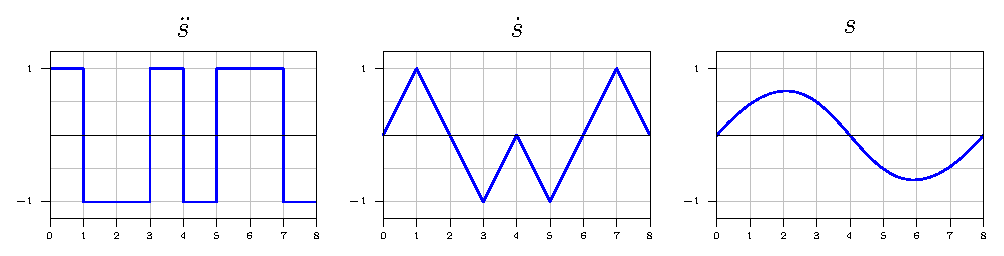
\includegraphics[width=1\textwidth ]{images/profiles.eps} 
\end{center}
Now we consider the \textit{control aspects} of the problem, we denote $\mathbf p_e(t)$ the position of the end effector at the time $t$, and $\mathbf p_d(t)$ the \textbf{desired position} at time $t$.\begin{equation}
    \mathbf p_d(0)=\mathbf p_a.
\end{equation}
We define the \textbf{error} such as the difference between the current position and the desired position:\begin{eqnarray}
    \mathbf e(t)=\mathbf p_d(t)-\mathbf p_e(t)
\end{eqnarray}
The aim of the \textit{control system} of the robot is to maintain $\mathbf e$ as close to zero as possible. This can be done by computing the initial error, and by giving to the system a new command $\dot\btheta(t)$ to correct it such that $\mathbf e(t)\rightarrow\mathbf 0$. Let's denotate the error as follows\begin{equation}
    \mathbf e(t)=\begin{pmatrix}
        e_x(t)\\ e_y(t)
    \end{pmatrix}
\end{equation}
For now, we will not discuss in detail how to control the error through the control of joint velocities $\dot\btheta$; it is sufficient to know that the following condition is required:\begin{equation}
    \dot{\mathbf e}(t)=-K\mathbf e(t)=\begin{pmatrix}
        -k_x&0\\
        0&-k_y
    \end{pmatrix}\begin{pmatrix}
        e_x(t)\\ e_y(t)
    \end{pmatrix}
\end{equation}
with $k_x,k_y>0$.
Why this conditions is required?\begin{itemize}
    \item if $e_x(t)$ is greater than zero, the condition $\dot e_x(t)=-k_xe_x(t)$ describes a decrease in error, making it approach zero 
    \item if $e_x(t)$ is smaller than zero, the condition $\dot e_x(t)=-k_xe_x(t)$ describes an increase in error, making it approach zero 
    \item same for $e_y$.
\end{itemize}
The system of equations\begin{equation}
    \dot{\mathbf e}(t)=\begin{pmatrix}
        -k_x&0\\
        0&-k_y
    \end{pmatrix}\begin{pmatrix}
        e_x(t)\\ e_y(t)
    \end{pmatrix}\implies \begin{cases}
        \dot e_x(t)=-k_xe_x(t)\\
        \dot e_y(t)=-k_ye_y(t)
    \end{cases}
\end{equation}
admits exponential functions as a solution\begin{align}
    &e_x(t)=e_x(0)e^{-k_xt}\\
    &e_y(t)=e_y(0)e^{-k_yt}
\end{align}
if the initial error $\mathbf e(0)$ is not zero, then the error will approaches zero, without never reaching it. For practical applications it goes sufficiently
fast to values very close to zero.\bigskip

\noindent We introduce now an important concept in linear differential equations systems.\begin{definition}
    Let $A\in M_{n,n}(\R)$ to be a squared real-valued matrix. The \textbf{matrix exponential}, denoted $e^A$, is the $n\times n$ matrix defined as follows:\begin{equation}
        e^A=\sum_{k=0}^\infty\frac{A^k}{k!}
    \end{equation}
\end{definition}
Given a linear system\begin{equation}
    \dot{\mathbf x}=A\mathbf x
\end{equation}
the solution is\begin{equation}
    \mathbf x(t)=e^{At}\mathbf x(0)
\end{equation}
In some cases the exponential matrix can be computed easily, let's assume that $A$ is diagonal\begin{equation}
    A=\begin{pmatrix}
a_1 & 0 & \cdots & 0 \\
0 & a_2 & \cdots & 0 \\
\vdots & \vdots & \ddots & \vdots \\
0 & 0 & \cdots & a_n
\end{pmatrix}
\end{equation}
in this case we have that\begin{equation}
    A^k=\begin{pmatrix}
a_1 & 0 & \cdots & 0 \\
0 & a_2 & \cdots & 0 \\
\vdots & \vdots & \ddots & \vdots \\
0 & 0 & \cdots & a_n
\end{pmatrix}\times  \dots \times \begin{pmatrix}
a_1 & 0 & \cdots & 0 \\
0 & a_2 & \cdots & 0 \\
\vdots & \vdots & \ddots & \vdots \\
0 & 0 & \cdots & a_n
\end{pmatrix} = \begin{pmatrix}
a_1^k & 0 & \cdots & 0 \\
0 & a_2^k & \cdots & 0 \\
\vdots & \vdots & \ddots & \vdots \\
0 & 0 & \cdots & a_n^k
\end{pmatrix}
\end{equation}
so\begin{align}
    &e^A=\sum_{k=0}^\infty\frac{1}{k!}\begin{pmatrix}
a_1^k & 0 & \cdots & 0 \\
0 & a_2^k & \cdots & 0 \\
\vdots & \vdots & \ddots & \vdots \\
0 & 0 & \cdots & a_n^k
\end{pmatrix}=
\begin{pmatrix}
\sum_{k=0}^\infty\frac{a_1^k}{k!} & 0 & \cdots & 0 \\
0 & \sum_{k=0}^\infty\frac{a_2^k}{k!} & \cdots & 0 \\
\vdots & \vdots & \ddots & \vdots \\
0 & 0 & \cdots & \sum_{k=0}^\infty\frac{a_n^k}{k!}
\end{pmatrix}\\& =
\begin{pmatrix}
e^{a_1} & 0 & \cdots & 0 \\
0 & e^{a_2} & \cdots & 0 \\
\vdots & \vdots & \ddots & \vdots \\
0 & 0 & \cdots & e^{a_n}
\end{pmatrix}.
\end{align}
So, if a system is described by a diagonalizable matrix $A$ there exists a diagonal matrix 
$\Lambda$ and an invertible matrix $T$ such that\begin{equation}
    A=T\Lambda T^{-1}
\end{equation}
in this case we can easily calculate the exponential matrix\begin{equation}
    e^{At}=T^{-1}e^{\Lambda t} T.
\end{equation}

\noindent\textbf{Note}: The Sections  \ref{gemini:def}, \ref{gemini:ethical}, \ref{gemini:ev}, \ref{gemini:examples}, \ref{gemini:statistics} are written with the aid of Gemini, by having the model process the information taken from the professor's slides and the lecture notes.

\section{Defining Robots}\label{gemini:def}
The concept of a robot is formalized through several key definitions, spanning from strict industrial standards to more encompassing theoretical perspectives.

\subsection{Standardized Definitions}

\subsubsection*{1. Industrial Definition (Robotic Institute of America - RIA)}
The RIA defines a robot as a \textbf{re-programmable, multi-functional manipulator} designed to move material, parts, tools, or specialized devices through variable programmed motions for the performance of a variety of tasks. A crucial element of this definition is the requirement that the robot must \textbf{acquire information from the environment} and move intelligently in response, setting it apart from simpler automated machinery.

\subsubsection*{2. ISO 8373:2012 Definition}
The International Organization for Standardization (ISO) provides a formal, international standard: an industrial robot is an \textbf{automatically controlled, re-programmable, multi-purpose manipulator} programmable in \textbf{three or more axes}. The manipulator may be either \textbf{fixed in place or mobile} and is intended for use in industrial automation applications. This specific definition helps to delineate complex, versatile machines from basic mechanical devices.

\subsection{The Visionary Definition: Perception and Action}
A broader, more "visionary" definition emphasizes the cognitive and functional aspects of robotic systems: the \textbf{intelligent connection between perception and action}.

\begin{itemize}
    \item \textbf{Perception:} This is the process of acquiring and processing sensing information from the environment.
    \item \textbf{Action:} This involves not just controlling the robot's current state, but actively \textbf{making some changes in the physical world} to achieve a goal.
\end{itemize}

This relationship forms a continuous feedback loop that governs autonomous behavior:
$$\text{percept} \longrightarrow \text{action} \longrightarrow \text{percept}$$
The robot's understanding of its environment (\textit{percept}) drives its movement or operation (\textit{action}), which modifies the environment, leading to a new cycle of perception.

\section{Notable Robot Examples}\label{gemini:examples}
Throughout history, various robots have exemplified different facets of the definition of robotics, from pure industrial work to exploration and human interaction.

\begin{itemize}
    \item \textbf{Comau H4 (1995):} Representing the industrial segment, these manipulators were widely used in \textbf{automotive industries} (e.g., owned by Fiat at the time). They are a classic example of fixed, multi-functional, re-programmable automation.
    
    \item \textbf{Waseda WAM-8 (1984):} This famous \textbf{humanoid robot} from a Japanese university demonstrated early cognitive abilities. It was capable of complex tasks such as playing an organ and reading music from a sheet, combining perception (reading) and fine manipulation.
    
    \item \textbf{Spirit Rover (2002):} An excellent example of \textbf{autonomous mobile robotics and exploration}.
    \begin{itemize}
        \item It was landed on Mars, featuring articulated wheels and solar panels.
        \item Its mission was to move, analyze material, and send gathered information back to Earth.
        \item While the \textbf{global target} is \textbf{specified remotely}, the rover must operate with significant \textbf{local autonomy} because of the approximately 8-minute communication delay required to receive instructions from Earth. This necessity highlights the critical role of the onboard perception-action loop for mission success.
    \end{itemize}
\end{itemize}
\begin{figure}[h!]
    \centering
    \includegraphics[width=0.4\textwidth ]{images/rover.jpg} 
    \caption{Spirit Rover (2002)}
\end{figure}

According to the rigorous \textbf{ISO 8373:2012} definition, certain devices and systems are \textbf{not considered robots}. These exclusions are typically applied to specific devices with only \textbf{one or two degrees of freedom (DOF)} and complex software systems lacking the physical manipulator required by the standard.
Systems that are not classified as robots under the ISO 2012 standard include:
\begin{itemize}
    \item Software ''bots'', Artificial Intelligence (AI), and Robotic Process Automation (RPA).
    \item Voice assistants.
    \item Automatic Teller Machines (ATMs).
    \item Cooking machines, smart washing machines, and similar appliances.
\end{itemize}
Furthermore, advanced mobile systems like drones and autonomous cars are generally not classified as robots under this definition. However, in a \textbf{2021 revision}, the term \textbf{robotic device} was introduced to encompass these increasingly sophisticated, automated machines that fall outside the strict definition of an industrial robot.\bigskip


The word ''robot'' has an historical and literary origin that is foundational to the field:
\begin{itemize}
    \item The term derives from the Slavic word \textbf{Robota}, meaning ''work'' or ''forced labor.''
    \item The first recorded use of the word ''Robot'' in a theatrical context was in \textbf{1920} by Czech writer \textbf{Karel Čapek} in his science-fiction play, \textit{Rossum's Universal Robots (R.U.R.)}. In the play, ''robots'' are artificial, human-like creatures created to be inexpensive workers.
\end{itemize}

\section{The Ethical Framework: Asimov's Three Laws of Robotics}\label{gemini:ethical}
The science fiction author Isaac Asimov defined a set of foundational ethical rules for robotics in his short stories.

\begin{enumerate}
    \item \textbf{First Law:} A robot may not injure a human being or, through inaction, allow a human being to come to harm.
    \begin{itemize}
        \item This law is fundamental to modern \textbf{collaborative robotics} (cobots), ensuring human safety is prioritized as robots and humans work in close proximity.
    \end{itemize}
    \item \textbf{Second Law:} A robot must obey orders given to it by human beings, except where such orders would conflict with the First Law.
    \begin{itemize}
        \item This establishes the robot's subordination to human command. Situations like robots used in war or faulty programming clearly violate this rule.
    \end{itemize}
    \item \textbf{Third Law:} A robot must protect its own existence as long as such protection does not conflict with the First or Second Law.
    \begin{itemize}
        \item The robot's self-preservation is conditional, being secondary to human safety and commands.
    \end{itemize}
\end{enumerate}

\section{Evolution and Characteristics of Robot Manipulators}\label{gemini:ev}

The journey toward the industrial robot began around the 1950s with the convergence of \textbf{Computerized Numerically Controlled (CNC) machines} and \textbf{mechanical telemanipulators}. This synthesis led to the development of the first \textbf{robot manipulators}, with the \textbf{Unimation PUMA (1970)} being a key early example.\bigskip


Unlike the early mechanical telemanipulators, which often required continuous human control, true robot manipulators offered several distinct advantages:
\begin{itemize}
    \item \textbf{Absence of Position Memory:} The robot operates based on its programmed coordinates, not needing to remember past states.
    \item \textbf{Adaptivity} to conditions previously unknown.
    \item High \textbf{Accuracy} in positioning.
    \item Superior \textbf{Repeatability} of operation (the ability to return consistently to a programmed point).
\end{itemize}
For an industrial manipulator, it is often noted that \textbf{repeatability} and \textbf{compliance} (adaptivity to variations) are more fundamental for task success than absolute accuracy.\bigskip

The history of industrial robotics is marked by key patented designs and technological firsts:
\textbf{The First Industrial Robot}
The very first industrial robot was installed at a General Motors plant in \textbf{1961}. It was developed by \textbf{George Devol and Joseph Engelberger} of Unimation.
\begin{itemize}
    \item \textbf{Kinematics:} This design featured a total of \textbf{6 Degrees of Freedom (DOF)}, comprising five revolute (rotational) joints and one prismatic (linear) joint. This combination was considered the optimal solution at the time to achieve \textbf{full control over the end effector's pose} (position and orientation).
\end{itemize}

\textbf{Key Successor Robot Manipulators}
Following the first installation, several robots introduced foundational innovations:
\begin{itemize}
    \item \textbf{ASEA IRB-6 (1973):} The first robot where all axes were driven by \textbf{electric motors} (all-electric drives), featuring 5 DOF.
    \item \textbf{Cincinnati Milacron T3 (1974):} Recognized as the first industrial robot to be controlled by a \textbf{micro-computer}.
    \item \textbf{Hirata AR-300 (1978):} Introduced the first \textbf{SCARA (Selective Compliance Assembly Robot Arm)} robot, which has a distinct cylindrical workspace, prioritizing speed and rigidity in the vertical axis.
    \item \textbf{Unimation PUMA 560 (1979):} Characterized by its 6 revolute joints, this was the first truly \textbf{'anthropomorphic'} robot, offering human-like dexterity.
\end{itemize}\bigskip

\begin{figure}[h!]
    \centering
    \includegraphics[width=0.4\textwidth ]{images/unimation.jpg} 
    \caption{Unimation PUMA 560 (1979)}
\end{figure}

Actuators power the robot and sustain its payload. \textbf{Electric motors} are the most common choice, converting electrical energy to torque. However, when required to sustain a \textbf{heavy payload}, a \textbf{hydraulic actuator} generally works better due to its higher power-to-weight ratio.
\section{Global Industrial Robotics Market Statistics}\label{gemini:statistics}

The following statistics are sourced from the \textbf{International Federation of Robotics (IFR)} World Robotics documents (Executive Summary for 2025 statistics). These figures illustrate the rapid global expansion of industrial automation.

\subsection{Operational Stock and Growth Rates}
The total worldwide operational stock of industrial robots reached \textbf{4.6 million units} at the end of 2024. This represents a substantial growth of \textbf{+9\%} compared to 2023. Over the five-year period from 2019 to 2024, the market demonstrated a robust Compound Annual Growth Rate (\textbf{CAGR}) of \textbf{+11\%}.

The Compound Annual Growth Rate is calculated as:
$$\text{CAGR} = \left(\frac{V_{\text{end}}}{V_{\text{begin}}}\right)^{1/\text{years}} - 1$$

New robot sales in 2024 reached \textbf{542,000 units}, maintaining stability ($\pm 0\%$) compared to 2023, and demonstrating a $+7\%$ CAGR from 2019–2024. This marks the \textbf{fourth consecutive year} that annual new installations have surpassed 500,000 units. The estimated average service life of an industrial robot is between \textbf{12 and 15 years}.

Regarding market size, the value of the robot market (excluding software and peripherals) was \textbf{\$15.7 billion} in 2022. The value of the total robotic systems market, which includes surrounding equipment and services, is estimated to be approximately \textbf{four times} this core market value.

\subsection{Sectoral and Geographic Distribution}
The market growth is primarily driven by the \textbf{electronics} and \textbf{automotive} industries, with collaborative robots (cobots) also contributing significantly to market expansion.

The global distribution of installations is highly concentrated:
\begin{itemize}
    \item \textbf{China} is the world's largest market for new installations, a position it has held since 2013. China installs \textbf{every other robot} globally, accounting for \textbf{54\%} of all new annual installations.
    \item A vast majority—\textbf{80\%} of all new robot installations—occur in just five countries: \textbf{China, Japan, USA, Korea, and Germany}.
    \item Within Europe, \textbf{Italy} stands out as the second-largest European country for new installations.
\end{itemize}

The scale of growth is highlighted by the historical operational stock data: starting from a modest 3,000 units in 1973, stock grew to 66K in 1983, 575K in 1993, and 800K in 2003, culminating in the 4.6 million units recorded in 2024.

\begin{figure}[h!]
    \centering
    \includegraphics[width=0.9\textwidth ]{images/op_stocks.png} 
\end{figure}

\chapter{Sensors and Actuators}
From an high level prospective, a robot is a system composed by different units, that takes commands and responds with actions in a working environment, as shown in figure \ref{fig:system}.
\begin{figure}[h!]
    \centering
    \includegraphics[width=0.7\textwidth ]{images/robosystem.png} 
    \caption{Robot as a system}
    \label{fig:system}
\end{figure}

The functional units are the following:\begin{itemize}
    \item mechanical units (robot arms): We see the links as rigid bodies, connected by rotational or prismatic joints, with an end effector attached at the end of the serial structure.
    \item actuation units: we have motors for the joints, that can be electrical, hydraulic or pneumatic, and eventually transmissions (i.g. a belt). We also consider the motion control algorithm as a part of that unit.
    \item sensor units: proprioceptive sensors that measure the internal state of the robot (position and velocity of the joints) and exteroceptive that measure the external environment.
    \item supervision units: AI and reasoning, task planning and control.
\end{itemize}
Let's focus on the actuation system, we can consider the scheme in figure \ref{fig:Actuationsystem}. We see how the power is measured in different units in different stage of the actuation process:\begin{itemize}
    \item Electrical : power = voltage $\times$ current
    \item Hydraulic : power = pressure $\times$ flow rate 
    \item Linear Mechanics : power = force $\times$ speed 
    \item Rotational Mechanics : power = torque $\times$ angular speed
\end{itemize}
{fig:system}.

\begin{figure}[h!]
    \centering
    \includegraphics[width=0.7\textwidth ]{images/actuation_system.png} 
    \caption{Actuation system}
    \label{fig:Actuationsystem}
\end{figure}


We define the efficiency as the ratio between the output and input power:\begin{equation}
    \text{efficiency}=\frac{P_u}{P_c}.
\end{equation}
\section{Electrical Motors}
Since pneumatic system have difficulties to guarantee  high levels of precision, and the hydraulic actuation systems are expensive and needs hydraulic supply, in most of the cases electrical servo motors are mounted on the robots.\begin{itemize}
    \item advantages of electrical motors:\begin{itemize}
        \item power supply available everywhere
        \item low cost
        \item large variety of products
\item high power conversion efficiency
\item easy maintenance
\item no pollution in working environment
    \end{itemize}
    \item disadvantages\begin{itemize}
        \item overheating in static conditions (in the presence of gravity)
\item need special protection in flammable environments
\item some advanced models require more complex control laws
    \end{itemize}
\end{itemize}\begin{center}
    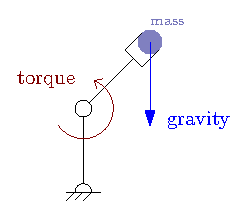
\includegraphics[width=0.25\textwidth ]{images/overheating.eps} 
\end{center}
If a robot should keep an object in a still position, the force of gravity tends to rotate the arms, so torque from the motors must be applied to keep that positions (this does not happen with hydraulic motors).
\begin{definition}
    A \textbf{servomotor} is a type of electric motor (AC or DC) specifically designed for the precision control of position, speed, and acceleration. It uses a closed-loop system with a feedback component (such as an encoder) that continuously monitors the motor's current position and compares it to the desired position. If there is a difference (an error signal), the controller corrects it, ensuring extremely accurate and dynamic motion.
\end{definition}
Desired characteristics for a servomotor mounted on a robot are:\begin{itemize}
    \item low inertia and high power-to-weight ratio
    \item high acceleration capabilities and large  range of operational velocities (1 to 2000 round per minute)
    \item low torque ripple\footnote{Torque ripple is an issue that arises in motors due to their construction, and it will be explained later.} and high accuracy in positioning
    \item power: 10 W to 10 kW.
\end{itemize}
There are two types of electrical motors\begin{itemize}
    \item Brushed DC: Has windings on the rotor (rotating part) and permanent magnets on the stator (stationary part). It uses physical brushes rubbing against a commutator to mechanically switch the current direction and maintain rotation.
    \item Brushless DC (BLDC): Has permanent magnets on the rotor and windings on the stator. It uses an electronic controller (instead of brushes/commutator) to electrically switch the current to the windings for rotation.
\end{itemize}\begin{center}
    \includegraphics[width=0.7\textwidth ]{images/brush_brushless.png} 
\end{center}


The DC motor has a complex construction, but the mathematical model that describes it is simple. The rotor (the rotating part) includes copper windings (coils) through which current circulates in a determined direction; power is supplied thanks to the contact of brushes that rub against the motor. The entire assembly is immersed in a magnetic field provided by permanent magnets, as shown in figure \ref{fig:motor}.\bigskip

\begin{figure}[h!]
    \centering
    \includegraphics[width=0.6\textwidth ]{images/motore2.eps}
    \caption{brush DC motor}
    \label{fig:motor}
\end{figure}

The electrons will move in the direction of the vector  
$\bar i$
(current density), with intensity I, and due to the presence of a magnetic field  
$\bar B$, they will be subjected to the \textbf{Lorentz force}
\begin{equation}
     \bar F = I(\bar l \times \bar B)
\end{equation}
where $\bar l$ represents the section of wire.
In this way, a torque will be generated, causing the circuit to rotate. The brushes, colored yellow in figure \ref{fig:motor}, by making contact, ensure that the current circulates. Note how the slip ring is divided into two parts; it acts as a \textit{commutator}. This construction allows the current to reverse direction with every half-turn. If this were not the case, the Lorentz force would alternate, causing the rotor to oscillate until it stopped, without rotating, as shown in figure \ref{fig:commutazione}.\bigskip

\begin{figure}[h!]
    \centering
    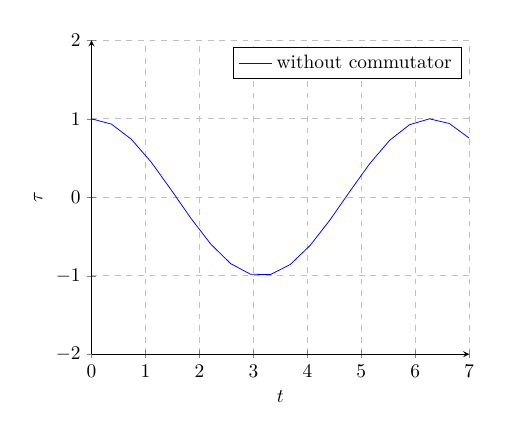
\begin{tikzpicture}[scale=0.7, transform shape]
        \begin{axis}[
        ymin=-2,
        ymax = 2,
        xmin=0,
        xmax = 7,
        axis lines = left,
        xtick distance=1, ytick distance=1,
        grid style=dashed,
        ymajorgrids=true,
        xmajorgrids=true,
        xlabel = \(t\),
        ylabel = {\(\tau\)},
        ]
        %Below the red parabola is defined
        \addplot [
        domain=0:7,
        samples=20,
        color=blue,
        ]
        {cos(deg(x))};
        \addlegendentry{without commutator}
        \end{axis}
        \end{tikzpicture}
        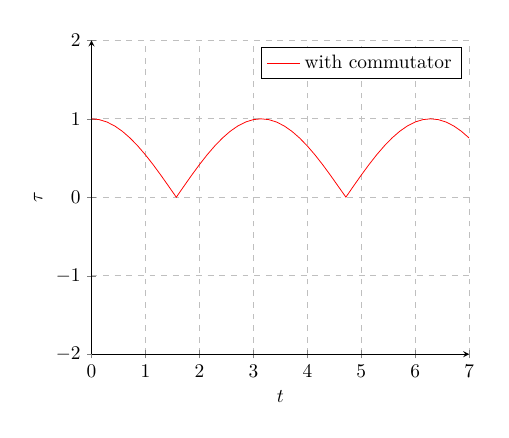
\begin{tikzpicture}[scale=0.7, transform shape]
        \begin{axis}[
        ymin=-2,
        ymax = 2,
        xmin=0,
        xmax = 7,
        axis lines = left,
        xtick distance=1, ytick distance=1,
        grid style=dashed,
        ymajorgrids=true,
        xmajorgrids=true,
        xlabel = \(t\),
        ylabel = {\(\tau\)},
        ]
        %Below the red parabola is defined
        \addplot [
        domain=0:7,
        samples=50,
        color=red,
        ]
        {abs(cos(deg(x)))};
        \addlegendentry{with commutator}
        \end{axis}
        \end{tikzpicture}
        \caption{Torque profile $\tau$}
        \label{fig:commutazione}
\end{figure}

\noindent The \textbf{torque} is equal to
\begin{equation}
    \bar T = (\bar r_1 \times  \bar F_1 + \bar r_2 \times  \bar F_2)
\end{equation}
We denote $\tau = \pm|\bar T|$ the \textit{scalar torque}.
\begin{center}
    \includegraphics[width=0.25\textwidth ]{images/momento.eps}
\end{center}
The force $\bar F$  depends on the angle $\theta$ of the motor's rotation, because the change in the direction of the current  
$\bar i$
  can cause the force to attenuate. The torque becomes zero every time the angle between the generated force and the lever arm of rotation is $k\pi$, where $k\in\N$.

\begin{center}
    \includegraphics[width=1\textwidth ]{images/variazioneCoppia.eps}
\end{center}
\begin{center}
	\begin{tabular}{>{\centering\arraybackslash}m{3in}>{\arraybackslash}m{3in}}
        \includegraphics[width=0.33\textwidth ]{images/variazioneCoppia2.eps} & Because of this, the torque has an oscillatory behavior and is not constant; this phenomenon is called \textbf{torque ripple}. To limit this (and increase the torque), multiple coils can be added so that, at the instant one coil produces zero torque, another coil produces maximum torque.
		\\
	\end{tabular}
\end{center}
\begin{center}
    \begin{figure}[h!]
       \centering
       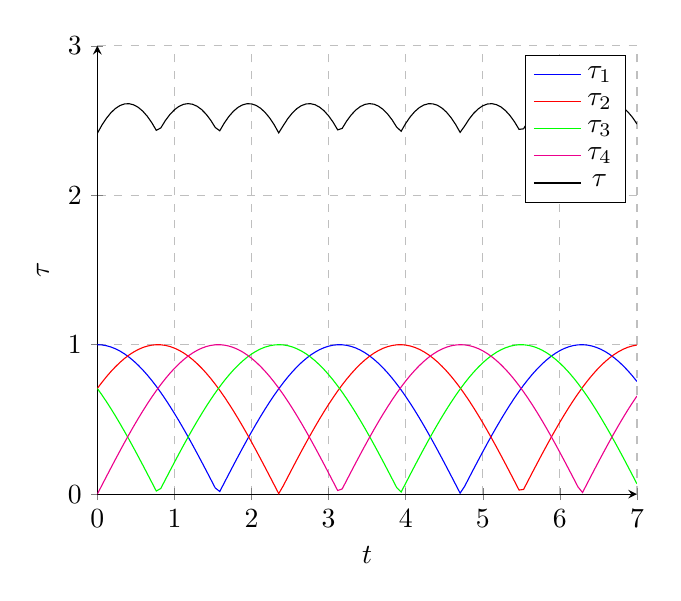
\begin{tikzpicture}[scale=1, transform shape]
           \begin{axis}[
           ymin=0,
           ymax = 3,
           xmin=0,
           xmax = 7,
           axis lines = left,
           xtick distance=1, ytick distance=1,
           grid style=dashed,
           ymajorgrids=true,
           xmajorgrids=true,
           xlabel = \(t\),
           ylabel = {\(\tau\)},
           ]
           %Below the red parabola is defined
           \addplot [
           domain=0:7,
           samples=120,
           color=blue,
           ]
           {abs(cos(deg(x)))};
           \addlegendentry{$\tau_1$}
           \addplot [
            domain=0:7,
            samples=120,
            color=red,
            ]
            {abs(cos((deg(x+((3/4)*pi)))))};
            \addlegendentry{$\tau_2$}
            \addplot [
            domain=0:7,
            samples=120,
            color=green,
            ]
            {abs(cos(deg(x+(pi/4))))};
            \addlegendentry{$\tau_3$}
            \addplot [
            domain=0:7,
            samples=120,
            color=magenta,
            ]
            {abs(cos(deg(x+(pi/2))))};
            \addlegendentry{$\tau_4$}
            \addplot [
            domain=0:7,
            samples=120,
            color=black,
            ]
            {abs(cos(deg(x+(pi/2))))+abs(cos(deg(x+(pi/4))))+abs(cos(deg(x+((3/4)*pi))))+abs(cos(deg(x)))};
            \addlegendentry{$\tau$}
           \end{axis}
           \end{tikzpicture}
           \caption{torque generated by multiple coils.}
        \end{figure}
    \end{center}
The greater the number of coils included, the more the torque ''flattens out'', tending towards a constant behavior.
\subsection{Dynamical Model of the Motor}
Now let's model an electric motor as a dynamical system. The motor is composed by two main sub-model\begin{itemize}
    \item An electromagnetic model 
    \item A mechanical model 
\end{itemize}
The commutator circuit have in series a resistor and an inductor, the model is shown in figure \ref{fig:model_motor}.

\begin{figure}[h!]
    \centering
    \includegraphics[width=0.8\textwidth ]{images/motor_scheme.drawio.pdf}
    \caption{Dynamical Model}
    \label{fig:model_motor}
\end{figure}

in the electromagnetic sub model, the voltage $v_a$ is given by the Kirchhoff laws\begin{equation}
    v_a(t)=R_ai_a(t)+L_a\frac{d i_a}{dt}+v_{emf}(t)
\end{equation}
where\begin{itemize}
    \item $R_a$ is the resistance coefficient 
    \item $L_a$ is the inductance. 
\end{itemize}
The term $v_{emf}(t)$ is called \textbf{Back Electromotive Force} and is a voltage generated within the rotating armature of an electric motor,  based on Faraday's Law of Induction, when the motor's armature coils $\omega(t)$ rotate and cut across the magnetic field (produced by the field coils or permanent magnets), a voltage is induced across the armature windings. Since a motor in motion is essentially acting as a generator, this is often called generator action. This voltage is proportional to the angular speed of the motor\begin{equation}\label{eq:model_balance_2}
    v_{emf}(t)=k_v\omega(t)
\end{equation}
Let's consider the mechanical sub model, we apply the newton law on torques, the scalar torque $\tau_m(t)$ of the rotating body is given by\begin{equation}
    \tau_m(t)=I_m\frac{d\omega}{dt}+F_m\omega(t)+\tau_{load}(t)
\end{equation}
where\begin{itemize}
    \item $I_m$ is the moment of inertia of the motor, a larger moment of inertia means the motor will take more torque and time to accelerate or decelerate to a given speed.
    \item $F_m$ is the viscous friction coefficient (since the motor never rotate in the void), and is proportional to the angular speed. It has a damping action on the rotational speed
    \item $\tau_{load}(t)$ is the external mechanical torque load given by the weight of the object that the motor is trying to rotate, and it opposes to the input torque.
\end{itemize}
The two sub models are related by an equation, it states that the torque $\tau_m$ of the motor is proportional to the applied current $i_a$ on the circuit:\begin{equation}\label{eq:model_balance}
    \tau_m(t)=k_ti_a(t)
\end{equation}
Let's define the state variables of our model, we can apply a voltage $v_a(t)$, and we are interested in the resulting angular position $\theta$ and speed $\dot\theta=\omega$.  \begin{align}
    &\begin{cases}
        \displaystyle v_a(t)=R_ai_a(t)+L_a\frac{d i_a}{dt}+v_{emf}(t)\\
        \displaystyle \tau_m(t)=I_m\frac{d\omega}{dt}+F_m\omega(t)+\tau_{load}(t)\\
    \end{cases}
\end{align}
by using the equations \eqref{eq:model_balance} and \eqref{eq:model_balance_2} we get
\begin{align}
    &\begin{cases}
        \displaystyle v_a(t)=R_ai_a(t)+L_a\frac{d i_a}{dt}+v_{emf}(t)\\
        \displaystyle k_ti_a(t)=I_m\frac{d\omega}{dt}+F_m\omega(t)+\tau_{load}(t)\\
    \end{cases}\implies \\ 
    &\begin{cases}
        \displaystyle L_a\frac{d i_a}{dt}=v_a(t)-R_ai_a(t)-k_v\omega(t)\\ 
        \displaystyle I_m\frac{d\omega}{dt}=k_ti_a(t)-F_m\omega(t)-\tau_{load}(t)\\
        \displaystyle \frac{d\theta}{dt}=\omega(t)
    \end{cases}
\end{align}
in the dot notation for derivatives:\begin{align}
   &\begin{cases}
        \displaystyle L_a\dot{i_a}=v_a(t)-R_ai_a(t)-k_v\omega(t)\\
        \displaystyle I_m\ddot\theta=k_ti_a(t)-F_m\omega(t)-\tau_{load}(t)\\
        \displaystyle \dot\theta=\omega(t)
    \end{cases}
\end{align}
the state variables are\begin{equation}
    \mathbf x  =\begin{pmatrix}
        \dot{i_a} \\ 
        \ddot \theta\\ 
        \dot \theta
    \end{pmatrix}
\end{equation}
the position $\theta$ can be found by integrating $\omega$. The motor is a system that given a input voltage over time $v_a(t)$, returns the electric current (more precisely, it's derivative, $i_a$ can be found by integrating over time), the angular speed  and the acceleration of the motor.\begin{center}
    \includegraphics[width=0.4\textwidth ]{images/motor_abstract.eps}
\end{center}
\begin{quote}
    \textbf{About the notation}: if $f(t)$ is a function in the time domain, we denote $\mathcal L[f](s)=f(s)$ it's Laplace transform in the complex variable $s$. For example: \begin{equation}
        \mathcal L[i_a](s)=i_a(s)
    \end{equation}
\end{quote}
Let's analyze the model in the Laplace domain by considering the Laplace transform, and then draw the block diagram of the system. For the electrical model we have\begin{align}
    &\mathcal L\left[ \displaystyle L_a\dot{i_a}=v_a(t)-R_ai_a(t)-k_v\omega(t) \right]\implies\\ 
    &sL_a i_a(s)=v_a(s)-R_ai_a(s)-k_v\omega(s)\implies\\
    &sL_a i_a(s)+R_ai_a(s)=v_a(s)-k_v\omega(s) \implies \\
    &(sL_a+R_a)i_a(s)=v_a(s)-k_v\omega(s) \implies\\
    &i_a(s)=\frac{v_a(s)-k_v\omega(s)}{sL_a+R_a}
\end{align}
assuming that the quantities are null in $t=0$. In the end, we get:\begin{equation}
    i_a(s)=\frac{v_a(s)-k_v\omega(s)}{sL_a+R_a}
\end{equation}
$v_a$ and $v_{emf}$ are external input to the model, so the transfer function for the electromagnetic sub model is\begin{equation}
    \frac{1}{sL_a+R_a}
\end{equation}
\begin{center}
    \includegraphics[width=0.7\textwidth ]{images/EM_model.drawio.pdf}
\end{center}
By analogous steps, we find that the transfer function for the mechanical sub model is\begin{equation}
    \frac{1}{sI_m+F_m}
\end{equation}
where the input is the torque $\tau_m$ from which we subtract the torque load $\tau_{load}$.
\begin{center}
    \includegraphics[width=0.7\textwidth ]{images/Mech_model.drawio.pdf}
\end{center}
We can chain the models since $\tau_m=k_ti_a$\begin{center}
    \includegraphics[width=1\textwidth ]{images/full_model.drawio.pdf}
\end{center}\begin{proposition}
    The two constants $k_v$ and $k_t$ are equals\begin{equation}
        k_v=k_t.
    \end{equation}
\end{proposition}
\textit{Proof}: This is trivially true. The electric power generated by the EM sub model is\begin{equation}
    v_{emf}i_a
\end{equation}
the mechanical power is\begin{equation}
    \tau_m\omega 
\end{equation}
since the conservation of power holds in energy transformations:\begin{equation}
    v_{emf}i_a= \tau_m\omega
\end{equation}
applying equations \eqref{eq:model_balance_2},\eqref{eq:model_balance} we get\begin{align}
    &v_{emf}i_a= \tau_m\omega\implies\\ 
    &k_v\omega i_a= k_ti_a\omega\implies \\ 
    &k_v=k_t. 
\end{align}
\hfill$\blacksquare$
\section{Transmissions}
We make use of motion transmission gears to:\begin{itemize}
    \item optimize the transfer of mechanical torque from actuating motors to driven links 
    \item quantitative transformation of torque/velocity, since these two can be controlled, by letting constant the ratio 
    \item qualitative transformation from rotational motion to linear (and vice versa)
    \item allow improvement of static and dynamic performance by
reducing the weight of the actual robot structure in motion
(locating the motors remotely, closer to the robot base)
\end{itemize}
There are different kinds of transmissions in robotics:\begin{itemize}
    \item \textbf{spur/bevel gears}: modify direction and/or translate
axis of motor displacement. \begin{itemize}
    \item \textit{Problems}: deformations, backlash
\end{itemize}
 \item \textbf{lead screws, worm gearing}: convert rotational
into translational motion (prismatic joints)\begin{itemize}
    \item \textit{Problems}: friction, elasticity, backlash
\end{itemize}
\item \textbf{toothed belts and chains}: dislocate the motor with respect to the joint axis\begin{itemize}
    \item \textit{Problems}: belts are subject to compliance and larger mass at high speed can induce vibrations to the chains.
\end{itemize}
\item \textbf{harmonic drives}: compact, in-line, power efficient,
with high reduction ratio (up to 150-200:1)\begin{itemize}
    \item \textit{Problems}: elasticity.
\end{itemize}\item\textbf{transmission shafts}: long, inside the links,
with flexible couplings for alignment
\end{itemize}
\begin{center}
    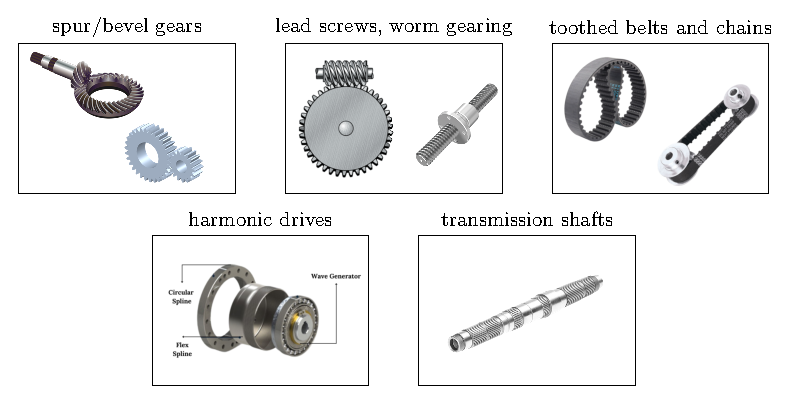
\includegraphics[width=1\textwidth ]{images/transmissions.eps}
\end{center}
\subsection{Harmonic Drives}
A Harmonic Drive, also known as a Strain Wave Gear, is a high-precision, compact gear system capable of achieving very high reduction ratios in a single stage, with near-zero backlash. They are widely used in robotics and aerospace.

The core of a Harmonic Drive mechanism involves the elastic deflection of a flexible gear component. It consists of three main components:\begin{enumerate}
    \item Wave Generator (Input): This is typically an elliptical plug fitted with a specialized, thin-raced ball bearing. It serves as the input element, usually attached to the motor shaft. As it rotates, its elliptical shape is transmitted to the next component.
    \item Flexspline (Output): A thin-walled, flexible metal cup with external gear teeth around its open edge. When the wave generator is inserted, the flexspline conforms to the elliptical shape, causing its teeth to engage with the circular spline at two opposite regions (the major axis of the ellipse) and disengage at the minor axis. The output shaft is typically connected to the rigid base of this cup.
    \item Circular Spline (Fixed): A rigid ring with internal teeth that meshes with the flexspline's external teeth. The key is that the Circular Spline has two more teeth than the Flexspline. It is usually fixed to the housing.
\end{enumerate}
Given\begin{itemize}
    \item $N_{CS}$ : number of inner teeth 
    \item $N_{FS}$ : number of outer teeth, $N_{CS}=N_{FS}+2$ since the Circular Spline typically has two more teeth than the Flexspline
\end{itemize}
the reduction ratio $n$ is\begin{equation}
    n=\frac{N_{FS}}{N_{CS}-N_{FS}}=\frac{N_{FS}}{2}
\end{equation}
\begin{center}
    \includegraphics[width=0.35\textwidth ]{images/harmonic_drives.png}
\end{center}
The video in the following link:\begin{quote}
    \url{https://www.youtube.com/watch?v=bzRh672peNk}
\end{quote}
shows in details how a harmonic drives works.
\subsection{Reduction Ratio}
We can see the transmission gear system as a black box that takes in input mechanical power $P_m$ from the motors, and gives in output mechanical power to the links $P_u$, the mechanical power in this context is given by the product of the torque generated by the motors and the angular speed:\begin{align}
    &P_m=\tau_m\dot\theta_m\\
     &P_u=\tau_u\dot\theta_u
\end{align}
there are some power that are dissipated due to the friction:\begin{equation}
    P_u = P_m-P_d, \ \ \ \ P_d>0
\end{equation}
in the ideal case there are no friction:\begin{equation}
    P_m=\tau_m\dot\theta_m=\tau_u\dot\theta_u=P_u
\end{equation}
every transmission gear have a reduction ratio $n$, such that\begin{align}
    &\dot\theta_m=n\dot\theta_u\\
    &\tau_u=n\tau_m
\end{align}
reducing the angular speed will increase the torque and vice versa.\bigskip 

\noindent 
Let's assume that we would like to provide a desired angular acceleration $\ddot\theta_u=a$ to the link trough the transmission gear, we have $$\ddot\theta_u=a\implies\ddot\theta_m=na$$
Let\begin{itemize}
    \item $J_m$ to be the moment of inertia of the motor 
    \item $J_u$ is the moment of inertia of the load
\end{itemize}
to achieve $\ddot\theta_u=a$ the motor should provide a torque
\begin{equation}
    \tau_m=J_m\ddot{\theta}_m+\frac{1}{n}(J_u\ddot\theta_u)=\left( J_mn+\frac{J_u}{n} \right)a
\end{equation}
we want to choose the ratio $n$ that minimize the sufficient torque $\tau_m$ to achieve $\ddot\theta_u=a$. We set\begin{align}
    &\frac{\partial \tau_m}{\partial n}=0\implies\\ &\left( J_m+\frac{J_u}{n^2} \right)a=0\implies \\ 
    &n=\sqrt{\frac{J_u}{J_m}}
\end{align}
\section{Sensors}
A measurement system should be \textbf{accurate}, the measured values should agree with the reference standard (usually given in ideal cases). Consecutive measurements of the same constant input quantity should reproduce similar measurement output (\textbf{repeatability}), and it should be \textbf{stable}, by keeping the same measuring characteristics over time. Usually\begin{itemize}
    \item better components leads to better repeatability 
    \item calibration leads to high accuracy
\end{itemize}
\begin{center}
    \includegraphics[width=0.65\textwidth ]{images/measurment.png}
\end{center}
There are other properties of a measurement system:\begin{itemize}
    \item the linearity error is the maximum deviation of the measured output from the
straight line that best fits the real characteristics, this is the ''error'' of the measurement system if we assume that the process that we are measuring produces output that are linear in the input.
    \item the offset error is the value of the measured output for the null input 
    \item the resolution error is maximum variation (measured in $\%$) of the input quantity producing no variation of the measured output
\end{itemize}
\begin{center}
    \includegraphics[width=0.45\textwidth ]{images/measurment2.png}
\end{center}
\subsection{Absolute and Incremental Encoders}
The \textbf{absolute encoders} are angular position sensors, highly used in robotics, these are optical sensor, that uses light pulses to measure the absolute angular position. An encoder works in the following way:\begin{itemize}
    \item there are a rotating optical disk, with alternate transparent and opaque sectors on multiple concentric tracks 
    \item a light beam are emitted, it passes trough these opaque and transparent sensor and then hits a photo-receiver 
    \item the intensity of the lights received depends on the tracks, in this way, the intensity is a measure of the position of the rotating part 
    \item light pulses are converted into
electrical pulses, electronically
processed and transmitted in output
\end{itemize}
\begin{center}
    \includegraphics[width=0.6\textwidth ]{images/encoder.jpg}
\end{center}
We denote $N_t$ the number of tracks, there is a digital encoding of the absolute position, stored in $N_t$ bits. The resolution of an absolute encoder is \begin{equation}
    \frac{360}{2^{N_t}}\text{ degrees}
\end{equation}
The alternation of opaque and transparent sectors leads to $2^{N_t}$ possible combination that can be detected.\bigskip 

The \textbf{incremental encoders} works differently, they have only 3 tracks, usually called $A,B$ and $Z$, alternating transparent and opaque areas. Instead of measuring the angular position, the lights detects angular displacements, each displacement (change of the light received) is a pulse, we denote $N_e$ the number of pulses per turn.\begin{itemize}
    \item The first two tracks $A$ and $B$ of the encoder are ''shifted'' and necessary to detect the rotation direction.
    \item The lights passes trough the two tracks and are received as two signals (one for each tracks).
\end{itemize}
\begin{center}
    \includegraphics[width=0.8\textwidth ]{images/incremental_encoder.png}
\end{center}
The third track $Z$ is used to define a zero reference position with a reset of the counter of the pulses. We define one \textbf{electrical degree} as\begin{equation}
    \frac{1 \text{ mechanical degree}}{N_e}
\end{equation}

360 electrical degrees (one full electrical turn) corresponds to $\frac{360}{N_e}$ mechanical degrees. The two signals $A$ and $B$ are shifted of $90^\circ$ electrical degrees.
In that case, the signals $A$ and $B$ are always out of phase of 90 degrees, if $A$ anticipates $B$, the rotation direction is clockwise, else, if $B$ anticipates $A$, is clockwise.\bigskip 

The resolution of the incremental encoder depends on the number of slits on the rotating disc.\begin{itemize}
    \item since the incremental encoder can count the pulses per second, we can count the pulses $C$ every $\Delta t$ seconds. The ''pulses speed'' is $$ f=\frac{C}{\Delta T}$$
    \item the resolution of the encoder, denoted $PPR$ is the number of pulses per each turn.
    \item we can compute the degrees for each pulses as $$ AR=\frac{360^\circ}{PPR}$$
    \item at this point $f$ is the number of pulses per second, $AR$ is the degrees per pulses, angular velocity is the number of degrees per second:\begin{equation}
        \omega=f\cdot AR=\frac{C}{\Delta T}\cdot\frac{360^\circ}{PPR}\ \ \frac{\text{degrees}}{\text{seconds}}
    \end{equation}
\end{itemize}
For example, if an encoder have a resolution  of $PPR=1000$ (every 1000 pulses, the motor performs one complete turn), the angular resolution is $\frac{360^\circ}{1000}=0.36^\circ$, if in an interval of $\Delta t=0.1$ seconds, we count $C=200$ pulses, the angular speed of the motor is\begin{equation}
    \frac{200}{0.1}\frac{360}{1000}=720\ \ \frac{\text{degrees}}{\text{seconds}}
\end{equation}
So every second the motor performs two complete revolutions.
\subsection{Quadrature}
For now, we described the ''pulses'' per second, in details, the encoder counts the rising edges of the signal $A$:\begin{center}
    \includegraphics[width=0.5\textwidth ]{images/pulses.eps}
\end{center}
in the image, in the interval $t\in [0,4]$, 2 pulses are detected, so the velocity is $\frac{2}{4}$ pulses per seconds. The angular resolution $AR$ is computed as the number of pulses (rising edges of the signal $A$) per round. We can increase the angular resolution, instead of counting the rising edges of $A$, we can count the rising and descending edges of the two signals $A$ and $B$, increasing the angular resolution by 4 times.
\begin{center}
    \includegraphics[width=0.5\textwidth ]{images/pulses2.eps}
\end{center}
In that case instead of counting 2 pulses, we detected 8 pulses by the two signals, in that case the angular resolution become 
\begin{equation}
    AR=\frac{360^\circ}{PPR\cdot 4}
\end{equation}
Since the pulses per revolut are 4 times greater then the PPR without counting the two signals. We recap the general procedure:\begin{enumerate}
    \item Every incremental encoder have a fixed number of slits, we denote $PPR$ (pulses per revolution) this number. This is the number of square waves generated for each complete revolution of the motor. 
    \item The angular resolution depends on the quadrature\begin{itemize}
        \item if we count as pulses the rising edges of the signal $A$, we have a $D=1$ encoding 
        \item if we count as pulses the rising edges of $A$ and $B$, we have $D=2$ as encoding 
        \item if we count as pulses the rising and descending edges of $A$ and $B$, we have $D=4$ as encoding
    \end{itemize}
    \item the angular resolution (degrees over pulses) is\begin{equation}
        AR=\frac{360^\circ}{PPR\cdot D}
    \end{equation}
\end{enumerate}
\chapter{Describing Orientation}
\section{Position and Orientation of a Rigid Body}
We have a base reference frame $RF_A=(\mathbf x_A,\mathbf y_A,\mathbf z_A)$, and a rigid body $B$ in the space, let's say that there is a fixed reference frame $RF_B=(\mathbf x_B,\mathbf y_B,\mathbf z_B)$ attached to a point of $B$, a vector ${}^A\mathbf p\in\R^3$ can describe the position of the whole body respect to the frame $RF_A$, and a $3\times3$ matrix is sufficient to describe the orientation of that body.
\begin{center}
    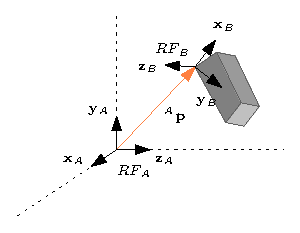
\includegraphics[width=0.5\textwidth ]{images/rigid_body_pose.eps}
\end{center}
The orientation of the reference frame $RF_B$ respect to $RF_A$ is described by a matrix $R$ of the following type\begin{itemize}
    \item $R$ is orthonormal, the columns vector are orthogonal from each other and have unitary length. 
    \item $R^T=R^{-1}\implies RR^T=I$
    \item $\det R=1$
\end{itemize}
These are the matrices in the orthogonal group $SO(3)$. More precisely, we denote ${}^AR_B$ the matrix that describe the orientation of $RF_B$ respect to $RF_A$. \begin{equation}
    {}^AR_B=\begin{pmatrix}
        &&\\
        {}^A\mathbf x_B&{}^A\mathbf y_B&{}^A\mathbf z_B\\
        &&
    \end{pmatrix}
\end{equation}
the components of ${}^AR_B$ are the direction cosines of the axes of $RF_B$ with respect to $RF_A$. In general, let's say the reference vector of two different frames are\begin{align}
    (\mathbf x_A,\mathbf y_A,\mathbf z_A)\\
    (\mathbf x_B,\mathbf y_B,\mathbf z_B)
\end{align}
the matrix ${}^AR_B$ is the following\begin{equation}
    {}^AR_B=\begin{pmatrix}
        \mathbf x^T_A\mathbf x_B&\mathbf x^T_A\mathbf y_B&\mathbf x^T_A\mathbf z_B\\ \\
        \mathbf y^T_A\mathbf x_B&\mathbf y^T_A\mathbf y_B&\mathbf y^T_A\mathbf z_B\\ \\
        \mathbf z^T_A\mathbf x_B&\mathbf z^T_A\mathbf y_B&\mathbf z^T_A\mathbf z_B
    \end{pmatrix}
\end{equation}
since all the basis vectors are unitary, and\begin{equation}
    \mathbf u^T\mathbf v=\|\mathbf u\|\cdot\|\mathbf v\|\cdot\cos\alpha
\end{equation}
we have that each component represent the angle between the two considered axis.
\begin{center}
    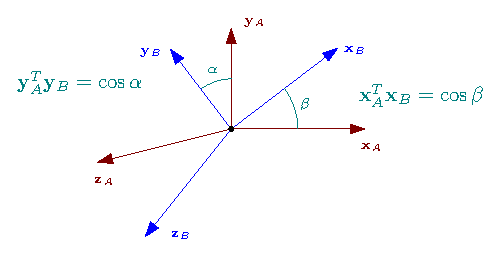
\includegraphics[width=0.6\textwidth ]{images/orientation_reference.eps}
\end{center}
for three different reference frame $RF_i,RF_j,RF_k$, the \textbf{chain rule} holds:\begin{equation}
    {}^kRF_i{}^iRF_j={}^kRF_j
\end{equation}
so, if ${}^A\mathbf p$ is a vector in the frame reference $RF_A$, the same vector in the reference frame $RF_B$ is\begin{equation}
    {}^B\mathbf p={}^BRF_A{}^A\mathbf p
\end{equation}
so the matrix is used for the \textbf{change of coordinates} between the two frames with different orientation.\begin{center}
    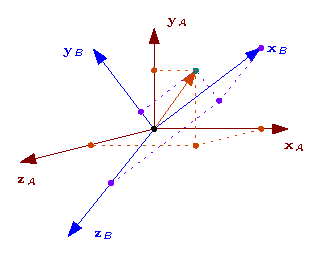
\includegraphics[width=0.5\textwidth ]{images/coordinate_change.eps}
\end{center}
The position of a rigid body can be expressed in cartesian, cylindrical or spherical coordinates. A point in $\R^3$ in cylindrical coordinates is described by\begin{equation}
    r,\theta,h 
\end{equation}
where the transformation from cylindrical to cartesian is\begin{align}
    &x=r\cos\theta\\
    &y=r\sin\theta\\
    &z=h 
\end{align}
the inverse transformation (assuming $r\ge 0$) is\begin{align}
    &r=\sqrt{x^2+y^2}\\ 
    &\theta =\text{atan2}(y,x)\\
    &h=z
\end{align}
The atan2$(y, x)$ function is a two-argument arctangent that returns the angle $\theta$ in standard position whose terminal side passes through the point $(x, y)$, correctly placing the angle in the correct quadrant ($\pi$ to $\pi$ or $0$ to $2\pi$). Is defined as follows;\begin{equation}
    \text{atan2}(y, x) =
\begin{cases}
\text{atan}\left(\frac{y}{x}\right) & x > 0 \\
\pi + \text{atan}\left(\frac{y}{x}\right) & y \geq 0, x < 0 \\
-\pi + \text{atan}\left(\frac{y}{x}\right) & y < 0, x < 0 \\
\frac{\pi}{2} & y > 0, x = 0 \\
-\frac{\pi}{2} & y < 0, x = 0 \\
\text{undefined} & y = 0, x = 0
\end{cases}
\end{equation}
We saw that the rotation matrices can describes the change of coordinates between two frames, and the orientation of a given frame with respect to another. These matrices can also describes the rotation of a vector in $\R^3$, let's consider a rotation around the $z$ axis. We have a vector $\mathbf v$ that lies in the $xy$ plane, with coordinates $$\mathbf v=\begin{pmatrix}
    x\\ 
   y\\z
\end{pmatrix}=\begin{pmatrix}
    \|\mathbf v\|\cos\alpha\\ 
    \|\mathbf v\|\sin\alpha\\z
\end{pmatrix}$$
where $\alpha$ is the angle between $\mathbf v$ and the $x$ axis. We rotate $\mathbf v$ by $\theta$ radiant around the $z$ axis, obtaining a new vector $\mathbf v'$ with coordinates$$
\mathbf v'=\begin{pmatrix}
    \|\mathbf v\|\cos(\alpha+\theta)\\ 
    \|\mathbf v\|\sin(\alpha+\theta)\\z
\end{pmatrix}=\begin{pmatrix}
    x\cos\theta-y\sin\alpha\\ 
    x\sin\theta+y\cos\alpha\\z
\end{pmatrix}
$$\begin{center}
    \includegraphics[width=0.35\textwidth ]{images/rotation_around_z.eps}
\end{center}
Notice how the relation between $\mathbf v$ and $\mathbf v'$ is given by a matrix $ \mathbf v'=R_z(\theta)\mathbf v$ called the \textbf{elementary rotation around $z$} by $\theta$ radiant.\begin{equation}
    R_z(\theta) =\begin{pmatrix}
        \cos\theta & -\sin\theta&0\\
        \sin\theta&\cos\theta&0\\
        0&0&1
    \end{pmatrix} 
\end{equation}
similarly, are defined elementary rotation around $x$ and $y$ too:\begin{equation}
     R_x(\theta) =\begin{pmatrix}
        1&0&0\\
        0&\cos\theta & -\sin\theta\\
        0&\sin\theta&\cos\theta
    \end{pmatrix}  \ \ \ \ \  
    R_y(\theta) =\begin{pmatrix}
        \cos\theta&0&\sin\theta\\ 0&1&0\\ -\sin\theta&0&\cos\theta
    \end{pmatrix} 
\end{equation}
So an orthonormal matrix have 3 possible interpretations:\begin{itemize}
    \item it can describe the orientation of a rigid body with respect to a reference frame
    \item it can describe the change of coordinates between two different frames one rotated respect to the other
    \item it can describe the rotation operator on a vector.
\end{itemize}
\subsubsection{Example}
Let's consider a sphere of radius $1$ as a rigid body, we have a reference frame $RF_S$ for the sphere fixed in the center, clearly the top pole in that frame is in position ${}^S\mathbf p=\begin{pmatrix}
    0&1&0
\end{pmatrix}^T$.\begin{center}
    \includegraphics[width=0.1\textwidth ]{images/sphere.eps}
\end{center}
We have a base frame $RF_0$ with the canonical base
$\mathbf e_x,\mathbf e_y,\mathbf e_z$, the sphere is placed in position $\begin{pmatrix}
    3&3&0
\end{pmatrix}^T$, we denote ${}^0\mathbf s$ the position of the frame $RF_S$ respect to $RF_0$. The sphere, is also rotated by 90 degrees clock wise around the $z$ axis.\begin{center}
    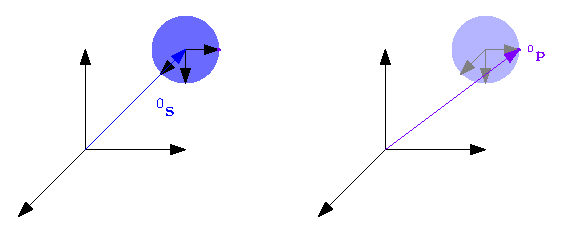
\includegraphics[width=0.7\textwidth ]{images/sphere_2.eps}
\end{center}
to find the position of the north pole $\mathbf p$ respect to $RF_0$, we have to apply the rotation matrix $R_z(-\nicefrac{\pi}{2})$ to ${}^S\mathbf p$ and consider the translation.
\begin{align}
    &{}^0\mathbf p=R_z(-\nicefrac{\pi}{2}){}^S\mathbf p+{}^0\mathbf s=\\
&\begin{pmatrix}
        0 & 1&0\\
        -1&0&0\\
        0&0&1
    \end{pmatrix} \begin{pmatrix}
    0\\1\\0
\end{pmatrix}+\begin{pmatrix}
    3\\3\\0
\end{pmatrix}=\begin{pmatrix}
    4\\3\\0
\end{pmatrix}.
\end{align}
Let's consider 4 reference frames $RF_0,RF_1,RF_2,RF_3$, with different orientations, we have 3 matrix$${}^0R_1,{}^1R_2,{}^2R_3$$
let's consider a position $\mathbf p$, in the coordinate system of $RF_3$, it's denoted ${}^3\mathbf p$, to express this position in $RF_0$ we can consider the matrix $$ {}^0R_1{}^1R_2{}^2R_3={}^0R_3$$
and we have$$ {}^0\mathbf p={}^0R_3{}^3\mathbf p$$
by getting this matrix products, we perform in total 63 products an 42 summations, we may calculate $ {}^0\mathbf p$ by deriving ${}^1\mathbf p$ and ${}^2\mathbf p$\begin{align}
    &{}^2\mathbf p = {}^2R_3{}^3\mathbf p\\ 
    &{}^1\mathbf p = {}^1R_2{}^2\mathbf p\\ 
    &{}^0\mathbf p = {}^0R_1{}^1\mathbf p
\end{align}
in this case, we perform in total 27 products an 18 summations, this is computationally better, in case we have to change the coordinates of multiple vector, is convenient to calculate the matrix ${}^0R_3$.
\section{Generalizing Rotation}
We defined the basic rotation along the three axis by an angle $\theta$\begin{equation}
    R_x(\theta),R_y(\theta),R_z(\theta)
\end{equation}
we want to generalize this concept by considering a rotation of $\theta$ radiants along an arbitrary direction $\mathbf r$ (with $\|\mathbf r\|=1$).
\begin{center}
    \includegraphics[width=0.4\textwidth ]{images/rotation.eps}
\end{center}
Given $\mathbf r,\theta$, we want to find the rotation matrix $R(\theta,\mathbf r)$ that describes the rotation of a vector of $\theta$ radiants along $r$, or the change of coordinates from a reference frame that is rotated in that orientation respect to the base frame.\begin{equation}
    \mathbf v'=R(\theta,\mathbf r)\mathbf v
\end{equation}
\subsection{Direct Problem}
We have to calculate $R(\theta,\mathbf r)\in SO(3)$ given $\theta,\mathbf r$. We can apply the following process:\begin{enumerate}
    \item We consider a transformation denoted $C$ that change the coordinate of our system, by making to set $\mathbf r$ aligned with the axis $z$.
    \item We consider the rotation along the $z$ axis by $\theta$ radiants. 
    \item We consider the inverse transformation of $C$ (since $C\in SO(3)$, $C^{-1}=C^T$).
\end{enumerate}
\begin{center}
    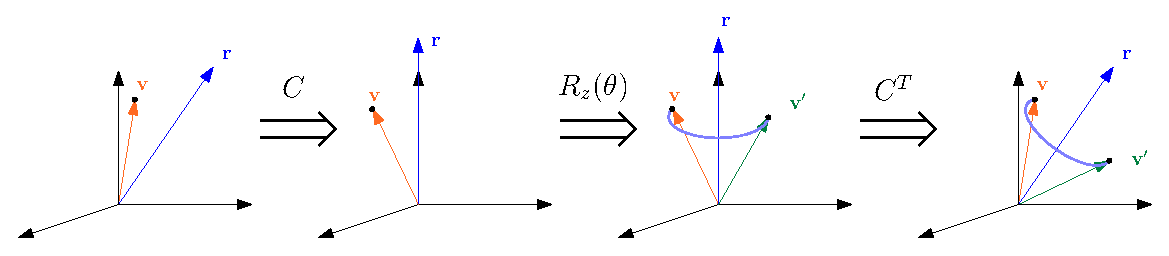
\includegraphics[width=\textwidth ]{images/CRC.eps}
\end{center}
In fact, we are looking for a rotation matrix $C$ such that\begin{equation}
    R(\theta,\mathbf r)=CR_z(\theta)C^T
\end{equation}
decomposing $ R(\theta,\mathbf r)$ in a sequence of three rotations. It's relevant to know that the third columns of $C$ is the vector $\mathbf r$\begin{equation}
    C=\begin{pmatrix}
        &&\\
        \mathbf n&\mathbf s&\mathbf r\\
        &&
    \end{pmatrix}
\end{equation}
Since $C\in SO(3)$, the vectors $ \mathbf n,\mathbf s,\mathbf r$ are orthogonal, and it holds that\begin{equation}
    \mathbf n\times \mathbf s =\mathbf r.
\end{equation}
Now we show how to get to $C$, by the fact that the column vectors are orthogonal, the inner product $C^TC$ is the identity matrix\begin{equation}
    \begin{pmatrix}
        
        &\mathbf n^T&\\ &\mathbf s^T& \\&\mathbf r^T&
        
    \end{pmatrix}
    \begin{pmatrix}
        &&\\
        \mathbf n&\mathbf s&\mathbf r\\
        &&
    \end{pmatrix}=I
\end{equation}
the \textbf{outer product} of two vectors $\mathbf v,\mathbf u\in\R^n$ is defined as follows\begin{equation}
    \mathbf v\mathbf u^T\in Mat(n\times n) 
\end{equation}
let $\mathbf e_i$ to be a vector of the canonical basis, the outer product \begin{equation}
    \mathbf e_i\mathbf e_j^T 
\end{equation}
is the $n\times n$ matrix with all entries equal to zeros, except for the $i,j$ entry, that is one, for example:\begin{equation}
   \mathbf e_1\mathbf e_3^T= \begin{pmatrix}
        1\\ 0\\ 0
    \end{pmatrix}\begin{pmatrix}
       0&0&1
    \end{pmatrix}=\begin{pmatrix}
        0&0&1\\ 
        0&0&0\\ 
        0&0&0
    \end{pmatrix}
\end{equation}
We define the \textbf{dyadic expansion} of an $n\times n$ matrix $A$ as the sum of $n^2$ matrices, in term of the entrance of that matrix\begin{equation}
    A=\sum_{i=1}^n\sum_{j=1}^n a_{ij}\mathbf e_i\mathbf e_j^T
\end{equation}
such that $a_{ij}$ is the $(i,j)$ entry of $A$. Note how \begin{equation}
    \sum_{i=1}^n\sum_{j=1}^n a_{ij}\mathbf e_i\mathbf e_j^T=IAI^T 
\end{equation}
the product of three matrices $B,A,B^T$ can be expressed in dyadic expansion as \begin{equation}
    BAB^T=\sum_{i=1}^n\sum_{j=1}^n a_{ij}\mathbf b_i\mathbf b_j^T
\end{equation}
Since $C\in SO(3)$, $CC^T=I$, with dyadic expansion:\begin{equation}
    CC^T=I= \begin{pmatrix}
        
        &\mathbf n^T&\\ &\mathbf s^T& \\&\mathbf r^T&
        
    \end{pmatrix}
    \begin{pmatrix}
        &&\\
        \mathbf n&\mathbf s&\mathbf r\\
        &&
    \end{pmatrix}= \begin{pmatrix}
        
        &\mathbf n^T&\\ &\mathbf s^T& \\&\mathbf r^T&
        
    \end{pmatrix}\begin{pmatrix}
        1&0&0\\ 
        0&1&0\\ 
        0&0&1
    \end{pmatrix}
    \begin{pmatrix}
        &&\\
        \mathbf n&\mathbf s&\mathbf r\\
        &&
    \end{pmatrix}=\mathbf n\mathbf n^T+
    \mathbf s\mathbf s^T+
    \mathbf r\mathbf r^T
\end{equation} 
the outer product of different vectors cancels out since are orthogonal from each other. We have that\begin{equation}
    \mathbf n\mathbf n^T+
    \mathbf s\mathbf s^T+
    \mathbf r\mathbf r^T=I.
\end{equation}
\begin{definition}
    A matrix $S\in Mat(n\times n)$ is \textbf{skew symmetric} if\begin{equation}
        S^T=-S
    \end{equation}
\end{definition}
The diagonal of a skew symmetric matrix have null entries. There are some notable properties:\begin{itemize}
    \item Any square matrix $A$ can be decomposed in a sum of two matrices, one symmetric, and one skew symmetric:\begin{equation}
        A=\frac{A+A^T}{2}+\frac{A-A^T}{2}
    \end{equation}
    where $\frac{A+A^T}{2}$ is symmetric and $\frac{A-A^T}{2}$ is skew symmetric. 
    \item In quadratic forms, only the symmetric part of a matrix influences the function:\begin{equation}
        \mathbf x^T A \mathbf x = \frac{1}{2}(\mathbf x^T A \mathbf x+(\mathbf x^T A \mathbf x)^T)=\frac{1}{2}(\mathbf x^T A \mathbf x+\mathbf x^T A^T \mathbf x)=\mathbf x^T\frac{A+A^T}{2}\mathbf x
    \end{equation}
    so only the symmetric part matters\begin{equation}
        \mathbf x^T A\mathbf x=\mathbf x^T\frac{A+A^T}{2}\mathbf x
    \end{equation}
    if follows that if $S$ is skew symmetric \begin{equation}
        \mathbf x^T S\mathbf x=\mathbf 0.   
    \end{equation}
\end{itemize}
The canonical form of a skew symmetric matrix is the following\begin{equation}
    S=\begin{pmatrix}
        0&-v_z&v_y\\ 
        v_z&0&-v_x\\ 
        -v_y&v_x&0
    \end{pmatrix}
\end{equation}
so to describe a matrix $S$ is sufficient a single vector \begin{equation}
    \mathbf v=\begin{pmatrix}
        v_x\\ 
        v_y\\ 
        v_z
    \end{pmatrix}
\end{equation}
in this way, given an arbitrary vector $\mathbf v\in \R^n$, we can construct the associated skew symmetric matrix $S(\mathbf v)\in Mat(n\times n)$.
\begin{proposition}
    Given two vectors $\mathbf v,\mathbf u$, the dot product $\mathbf v\times \mathbf u$ is equal to the product from the skew symmetric associated matrix $S(\mathbf v)$ and $\mathbf u$:\begin{equation}
        \mathbf v\times \mathbf u=S(\mathbf v)\mathbf u
    \end{equation}
\end{proposition}
Since $\mathbf v\times u=-\mathbf u\times \mathbf v$ and $-\mathbf u\times \mathbf v=-S(\mathbf u)\mathbf v$ it follows that \begin{equation}
    S(\mathbf v)\mathbf u = S^{T}(\mathbf u)\mathbf v.
\end{equation}
Let's go back to the original problem, given that $R(\theta,\mathbf r)=CR_z(\theta)C^T$, we want to derive $C$. Expanding the form we can see how\begin{align}
   & \begin{pmatrix}
        &&\\
        \mathbf n&\mathbf s&\mathbf r\\
        &&
    \end{pmatrix}
    \begin{pmatrix}
        \cos\theta&-\sin\theta&0\\ 
        \sin\theta&\cos\theta&0\\ 
        0&0&1
    \end{pmatrix}
    \begin{pmatrix}
        &\mathbf n^T&\\ &\mathbf s^T& \\&\mathbf r^T& 
    \end{pmatrix}=\\
    & \mathbf r\mathbf r^T+
    (\mathbf n\mathbf n^T+\mathbf s\mathbf s^T)\cos\theta+
    (\mathbf s\mathbf n^T-\mathbf n\mathbf s^T)\sin\theta
\end{align}
Since $CC^T= \mathbf r\mathbf r^T+
    \mathbf n\mathbf n^T+\mathbf s\mathbf s^T=I$, it implies that $\mathbf n\mathbf n^T+\mathbf s\mathbf s^T=I-\mathbf r\mathbf r^T$.\begin{align}
        &\mathbf r\mathbf r^T+
    (\mathbf n\mathbf n^T+\mathbf s\mathbf s^T)\cos\theta+
    (\mathbf s\mathbf n^T-\mathbf n\mathbf s^T)\sin\theta=\\ 
    &\mathbf r\mathbf r^T+
    (I-\mathbf r\mathbf r^T)\cos\theta+
    (\mathbf s\mathbf n^T-\mathbf n\mathbf s^T)\sin\theta
    \end{align}
It's important to notice that $\mathbf r$ is orthogonal to $\mathbf s$ and $\mathbf n$, and all three vectors are unit 1, it has to be that 
\begin{equation}
    \mathbf n \times\mathbf s =\mathbf r 
\end{equation}
so\begin{align}
     &\mathbf n \times\mathbf s =\begin{pmatrix}
        n_ys_z-s_yn_z\\ 
        n_zs_x-s_zn_x\\ 
        n_xs_y-s_xn_y
     \end{pmatrix}=\begin{pmatrix}
        r_x\\ r_y\\ r_z 
     \end{pmatrix}=\mathbf r
\end{align}
we can see how \begin{align}
    &\mathbf s\mathbf n^T-\mathbf n\mathbf s^T=\begin{pmatrix}
        0&-r_z&r_y\\
        r_z&0&-r_x\\ 
        -r_y&r_x&0 
    \end{pmatrix}=S(\mathbf r)
\end{align}
So $\mathbf s\mathbf n^T-\mathbf n\mathbf s^T$ is equal to the skew symmetric matrix associated to $\mathbf r$. Given these propositions, the following theorem holds.\begin{theorem}
    Given a vector $\mathbf r\in \R^3$ and an angle $\theta$, the rotation matrix that describes a rotation of $\theta$ radiants along the vector $\mathbf r$ is\begin{equation}
        R(\theta,\mathbf r)=\mathbf r\mathbf r^T+(I-\mathbf r\mathbf r^T)\cos\theta +S(\mathbf r)\sin\theta.
    \end{equation}
\end{theorem}
By developing all the computation we can expand the form of that matrix:\begin{equation}
     R(\theta,\mathbf r)=\begin{pmatrix}
r_x^2(1 - \cos \theta) + \cos \theta & r_x r_y(1 - \cos \theta) - r_z \sin \theta & r_x r_z(1 - \cos \theta) + r_y \sin \theta \\
r_x r_y(1 - \cos \theta) + r_z \sin \theta & r_y^2(1 - \cos \theta) + \cos \theta & r_y r_z(1 - \cos \theta) - r_x \sin \theta \\
r_x r_z(1 - \cos \theta) - r_y \sin \theta & r_y r_z(1 - \cos \theta) + r_x \sin \theta & r_z^2(1 - \cos \theta) + \cos \theta
\end{pmatrix}
\end{equation}
The trace of that matrix is $1+2\cos\theta$:\begin{equation}
    Trace(R(\theta,\mathbf r))=1+2\cos\theta
\end{equation}
and we have that\begin{equation}
    R(\theta,\mathbf r)=R(-\theta,-\mathbf r)=R^T(-\theta,\mathbf r)
\end{equation}
There are some properties of $ R(\theta,\mathbf r)$:\begin{itemize}
    \item Since is the rotation along $\mathbf r$, is invariant to $\mathbf r$\begin{equation}
         R(\theta,\mathbf r)\mathbf r = \mathbf r
    \end{equation}
    \item the map $(\theta,\mathbf r)\rightarrow  R(\theta,\mathbf r)$ is not injective since $R(\theta,\mathbf r)=R(-\theta,-\mathbf r)$
    \item if $\lambda_1,\lambda_2,\lambda_3$ are the eigenvalues of $R(\theta,\mathbf r)$, the determinant is\begin{equation}
        \det R = \lambda_1\lambda_2\lambda_3=1
    \end{equation}
    the trace is \begin{equation}
        \lambda_1+\lambda_2+\lambda_3=1+2\cos\theta
    \end{equation}
    one of the eigenvalues of $R$ is 1. Since $\lambda_2+\lambda_3=2\cos\theta$
    to find the other eigenvalues we can set the quadratic equation\begin{equation}
        \lambda^2+2\cos\theta\lambda+1=0 
    \end{equation}
    the two complex roots are\begin{equation}
        e^{\pm i\theta}
    \end{equation}
\end{itemize}\begin{center}
    \includegraphics[width=0.2\textwidth ]{images/eigenvalues.png}
\end{center}
Since $R$ is orthonormal, all eigenvalues have unitary norm.
\subsection{Inverse Problem}
Given a rotation matrix $R=(R_{ij})$, we want to find the unit vector $\mathbf r$ and the angle $\theta$ such that\begin{equation}
    R(\theta,\mathbf r)=(R_{ij})
\end{equation}
Since the trace is 
$R_{11}+R_{22}+R_{33}=1+2\cos\theta$, a possible solution for $\theta$ is\begin{equation}
    \theta=\arccos\frac{R_{11}+R_{22}+R_{33}-1}{2}
\end{equation}
this is not a good solution since $\arccos\in[0,\pi]$, and the function, when implemented, lacks of precision for $\theta$ near to 0. We can consider from the data $R$ that\begin{equation}
    R - R^{T} = \begin{pmatrix}
0 & R_{12} - R_{21} & R_{13} - R_{31} \\
R_{21} - R_{12} & 0 & R_{23} - R_{32} \\
R_{31} - R_{13} & R_{32} - R_{23} & 0
\end{pmatrix} = 2 \sin \theta \begin{pmatrix}
0 & -r_{z} & r_{y} \\
r_{z} & 0 & -r_{x} \\
-r_{y} & r_{x} & 0
\end{pmatrix}
\end{equation}
and since $\|\mathbf r \|$ we derive\begin{equation}
    \sin \theta = \pm \frac{1}{2} \sqrt{(R_{12} - R_{21})^2 + (R_{13} - R_{31})^2 + (R_{23} - R_{32})^2}
\end{equation}
so we can use the atan2 function\begin{equation}
    \text{atan2}(\pm \frac{1}{2} \sqrt{(R_{12} - R_{21})^2 + (R_{13} - R_{31})^2 + (R_{23} - R_{32})^2},R_{11}+R_{22}+R_{33}-1
    )
\end{equation}
if $\sin\theta\ne 0$, $\mathbf r$ is\begin{equation}
    \mathbf r=\frac{1}{2\sin\theta}\begin{pmatrix}
        R_{32}-R_{23}\\ 
        R_{13}-R_{31}\\
        R_{21}-R_{12}
    \end{pmatrix}
\end{equation}
if $\sin\theta=0$, we have two cases\begin{itemize}
    \item if $\theta=0$, there is no solution for $\mathbf r$
    \item if $\theta=\pm\pi$, we have $\sin\theta=0, \ \cos\theta=-1$ and we solve\begin{equation}
        R=2\mathbf r\mathbf r^T-I
    \end{equation}
    for $\mathbf r$.
\end{itemize}
\subsection{Quaternion Representation}
We can use quaternions to represent rotations, we will not enter in the algebraic details of the quaternions field, in this context, is sufficient to know that a quaternion is an element that can be described with a scalar and a vector in $\R^3$
\begin{align}
    &q=(\eta,\boldsymbol{\epsilon})\\
    &\eta\in\R\\ 
    &\boldsymbol{\epsilon}\in \R^3
\end{align}
We can represent a rotation along $\mathbf r$ of $\theta$ radiants by considering the quaternion\begin{align}
    q=(\cos\frac{\theta}{2},\sin\frac{\theta}{2}\mathbf r)
\end{align}
notice how $(\theta,\mathbf r)$ and  $(-\theta,-\mathbf r)$ are associated to the same quaternion. Given $q$, the rotation matrix is\begin{equation}\label{quat_mat}
    R(q)=R((\eta,\boldsymbol{\epsilon}))=\begin{pmatrix}
2(\eta^2 + \epsilon_x^2) - 1 & 2(\epsilon_x\epsilon_y - \eta\epsilon_z) & 2(\epsilon_x\epsilon_z + \eta\epsilon_y) \\
2(\epsilon_x\epsilon_y + \eta\epsilon_z) & 2(\eta^2 + \epsilon_y^2) - 1 & 2(\epsilon_y\epsilon_z - \eta\epsilon_x) \\
2(\epsilon_x\epsilon_z - \eta\epsilon_y) & 2(\epsilon_y\epsilon_z + \eta\epsilon_x) & 2(\eta^2 + \epsilon_z^2) - 1
\end{pmatrix}
\end{equation}
the inverse rotation of $q=(\eta,\boldsymbol{\epsilon})$ is $(\eta,-\boldsymbol{\epsilon})$, and the null rotation is $(1,\mathbf 0)$. There is a binary operation on quaternions $*$ such that\begin{equation}
    q_1*q_2=(\eta_1,\boldsymbol{\epsilon}_1)*
    (\eta_2,\boldsymbol{\epsilon}_2)=(\eta_1\eta_2-\boldsymbol{\epsilon}_1^T\boldsymbol{\epsilon}_2, \eta_1\boldsymbol{\epsilon}_2+\eta_2\boldsymbol{\epsilon}_1+\boldsymbol{\epsilon}_1\times \boldsymbol{\epsilon}_2)
\end{equation}
We also want to find the quaternion $q$ associated to a given rotation matrix $R=(R_{ij})$. Summing the elements on the diagonal of the matrix shown in \eqref{quat_mat} we get\begin{equation}
    R_{11}+R_{22}+R_{33}=4\eta^2-1
\end{equation}
the positive roots of this quadratic equation is the value of $\eta$\begin{equation}
    \eta=\frac{1}{2}\sqrt{R_{11}+R_{22}+R_{33}+1}\ge 0 
\end{equation}
without entering in the details, from the equation \eqref{quat_mat} we can derive the values for $\boldsymbol{\epsilon}$ as follows:\begin{align}
    &\epsilon_x=\frac{1}{2}\text{sign}(R_{32}-R_{23})\sqrt{R_{11}-R_{22}-R_{33}+1}\\
    &\epsilon_y=\frac{1}{2}\text{sign}(R_{13}-R_{32})\sqrt{R_{22}-R_{11}-R_{33}+1}\\
    &\epsilon_z=\frac{1}{2}\text{sign}(R_{21}-R_{12})\sqrt{R_{33}-R_{11}-R_{22}+1}
\end{align}
\section{Minimal Representations of Orientation}
We discussed many representation of rotation, quaternions, rotation axis and angle and  rotation matrices, we want to describe an orientation with the minimum number of variables, indeed, the group $SO(3)$ is a 3-manifold, to describe an element in $SO(3)$ we need just three independent variables. We define three rotation along the base axis with three angles $\alpha_1,\alpha_2,\alpha_3$.\bigskip 

There are two ways to use 3 angles to describe a rotation, one along moving axis, and one along fixed axis.
\subsection{Euler Angles}
We describe a rotation as a triple of angles $(\alpha_1,\alpha_2,\alpha_3)$, each angle is associated to an axis $X,Y$ or $Z$. The angle $\alpha_1$ describe a rotation of the frame along his associated axis, this will provide a new set of axis $X',Y',Z'$ with a different orientation respect to the initial one. The angle $\alpha_2$ describe a rotation of the frame along his associated axis in the new frame $X',Y',Z'$, this will provide a new frame $X'',Y'',Z''$, and  $\alpha_3$ describe a rotation of the frame along his associated axis in this last frame.\bigskip 

\noindent There are 12 possible sequence of axis for a rotation, for example\begin{itemize}
    \item $XY'X''$ describe a rotation along $X$, then $Y'$, and then $X''$. We use the quotation mark $'$ do emphasizes the fact that the axis is part of a frame that has been rotated.
    \item $ZX'Z''$ describe a rotation along $Z$, then $X'$, and then $Z''$.
\end{itemize}
We exclude  contiguous repetitions of axes, like $XX'Z''$ or $YZ'Z''$. Let's consider an example, we have the three euler angles $(\phi,\theta,\psi)$ associated to the axis $ZX'Z''$.
\begin{center}
    \includegraphics[width=\textwidth ]{images/eulerangles.eps}
\end{center}
The rotation matrix that describes this rotation is \begin{equation}
    R_z(\phi)R_{x}(\theta)R_z(\psi)
\end{equation}
\begin{definition}
    Given three euler angles $\alpha_1,\alpha_2,\alpha_3$ and three axis $$(a_1,a_2,a_3)  \ : \ a_i\in \{x,y,z\}, \ a_1\ne a_{2}, \ a_2\ne a_3
    $$
    the rotation matrix describing the rotation along this moving axes is\begin{equation}
        R_{a_1}(\alpha_1) R_{a_2}(\alpha_2) R_{a_3}(\alpha_3)
    \end{equation}
\end{definition}
For the example with the axis $ZX'Z''$, the expanded version of the matrix is the following\begin{equation}\label{ZXZ_mat}
    R=  \begin{pmatrix}
        \cos\phi\cos\psi-\sin\phi\cos\theta\sin\psi&-\cos\phi\sin\psi-\sin\phi\cos\theta\cos\psi&\sin\phi\sin\theta\\ 
        \sin\phi\sin\psi+\cos\phi\cos\theta\sin\psi&-\sin\phi\sin\psi+\cos\phi\cos\theta\cos\psi&-\cos\phi\sin\theta\\ 
        \sin\theta\sin\psi&\sin\theta\cos\psi&\cos\theta
    \end{pmatrix}
\end{equation}
Given a rotation matrix $R=(R_{ij})$, we can derive the values for $(\phi,\theta,\psi)$ by looking at the matrix in equation \eqref{ZXZ_mat}. Since \begin{align}
    &R_{13}=\sin\phi\sin\theta \\ 
    &R_{23}=-\cos\phi\sin\theta  
\end{align}
we have that \begin{align}
    &R_{13}^2+R_{23}^2=\sin^2\phi\sin^2\theta+(-\cos\phi)^2\sin^2\theta=\\ 
    &\sin^2\theta(\sin^2\phi+(-\cos\phi)^2)= \sin^2\theta(\sin^2\phi+\cos^2\phi)=\sin^2\theta\\ &\implies
    \sin\theta=\pm\sqrt{R_{13}^2+R_{23}^2}
\end{align}
and\begin{align}
    &R_{33}=\cos\theta  
\end{align}
we can derive $\theta$ with the atan2 function:\begin{equation}
    \theta=\text{atan2}\left(
        \pm\sqrt{R_{13}^2+R_{23}^2}, \ R_{33}
    \right).
\end{equation}
We have two possible values for $\theta$ since we have to consider that $\sin\theta=\pm\sqrt{R_{13}^2+R_{23}^2}$.
We consider the case without singularities, where $\sin\theta\ne 0$, since $R_{31}=\sin\theta\sin\psi$ and $R_{32}=\sin\theta\cos\psi$, we have that\begin{align}
    &\sin\psi=\nicefrac{R_{31}}{\sin\theta}\\ 
    &\cos\psi=\nicefrac{R_{32}}{\sin\theta}\\ 
    &\implies \psi=\text{atan2}\left(
        \frac{R_{31}}{\sin\theta}, \frac{R_{32}}{\sin\theta}
    \right).
\end{align}
By analogous steps, we can derive $\phi$:\begin{equation}
     \phi=\text{atan2}\left(
        \frac{R_{13}}{\sin\theta},- \frac{R_{23}}{\sin\theta}
    \right).
\end{equation}
Since we have two different values for $\theta$, this process provides two different triplets for the angles $(\phi,\theta,\psi)$. We have a singularity when\begin{equation}
    \theta=0\lor \theta=\pm\pi
\end{equation}
in that case, $\sin\theta=0$, so we can't derive the values for $\phi,\psi$. When $\sin\theta=0$, the rotation along the second axis $X'$ is irrelevant, we can't derive fixed values for $\psi,\phi$, but we can determine only the sum $\phi+\psi$ or the difference $\phi-\psi$. This fact should be intuitive, since we are not rotating along $X'$, we are doing two consecutive rotation along $Z=Z''$.
$$R=R_z(\phi+\psi)$$
This discussion concerns the specific case of rotations along $ZX'Z''$, analogous considerations can be made for all other cases.
\subsection{Roll-Pitch-Yaw Angles}
We describe a rotation as a triple of angles $(\alpha_1,\alpha_2,\alpha_3)$, each angle is associated to an axis $X,Y$ or $Z$. The frame gets rotated always along fixed axis, so, if we have a rotation along $ZXZ$ with angles $(\phi,\theta,\psi)$, the frame gets rotated by $\phi$ along $Z$, then by $\theta$ along the original axis $X$ and not the rotated one $X'$.\begin{center}
    \includegraphics[width=0.7\textwidth ]{images/rpy_angles.eps}
\end{center}
In this case\begin{enumerate}
    \item We perform a rotation along $Z$ with $R_z(\phi)$
    \item We perform a rotation along the original $X$, that is not coincident with the current axis $X'$, so the rotation matrix is $C_1R_x(\theta)C_1^T$
    \item We perform a rotation along the original $Z$, that is not coincident with the current axis $Z''$, so the rotation matrix is $C_2R_z(\psi)C_2^T$
\end{enumerate}
The final matrix is \begin{equation}
    R_z(\phi)C_1R_x(\theta)C_1^TC_2R_z(\psi)C_2^T
\end{equation}
\begin{theorem}
    $R_z(\phi)C_1R_x(\theta)C_1^TC_2R_z(\psi)C_2^T=R_z(\psi)R_x(\theta)R_z(\phi)$
\end{theorem}
\textit{Proof}: The rotation $C_1$ align the  axis $X'$ of the frame after the first rotation along $Z$ with the original axis $X$, so $$C_1=R^T_z(\phi).$$ Similarly, the transformation $C_2$ align the axis $Z''$ after two rotation with the original axis $Z$, so $$C_2=R^T_z(\phi)R^T_x(\theta).$$
We can expand the matrix \begin{align}
     &R_z(\phi)C_1R_x(\theta)C_1^TC_2R_z(\psi)C_2^T=\\ 
    &R_z(\phi)R^T_z(\phi)R_x(\theta)R_z(\phi)R^T_z(\phi)R^T_x(\theta)R_z(\psi)R_x(\theta)R_z(\phi)=\\ 
&\color{red}R_z(\phi)R^T_z(\phi)\color{black}R_x(\theta)\color{red}R_z(\phi)R^T_z(\phi)\color{black}R^T_x(\theta)R_z(\psi)R_x(\theta)R_z(\phi)=\\ 
&\color{red}R_x(\theta)R^T_x(\theta)\color{black}R_z(\psi)R_x(\theta)R_z(\phi)=\\ 
&R_z(\psi)R_x(\theta)R_z(\phi) \ \ \ \ \ \ \ \ \ \ \ \ \blacksquare
\end{align}
\begin{definition}
    Given three roll-pitch-yaw angles $\alpha_1,\alpha_2,\alpha_3$ and three axis $$(a_1,a_2,a_3)  \ : \ a_i\in \{x,y,z\}, \ a_1\ne a_{2}, \ a_2\ne a_3
    $$
    the rotation matrix describing the rotation along this fixed axes is\begin{equation}
        R_{a_3}(\alpha_3) R_{a_2}(\alpha_2) R_{a_1}(\alpha_1)
    \end{equation}
\end{definition}
The roll-pitch-yaw angles rotation is equivalent to an euler angles rotation, we get this equivalence by inverting the order of the sequence of axis:$$\begin{matrix}
    \begin{matrix}
        \textbf{Euler angles}\\ 
        \text{first rotation :  by }\alpha_1\text{ radiants along }a_1\\ 
        \text{second rotation :  by }\alpha_2\text{ radiants along }a_2\\ 
        \text{third rotation :  by }\alpha_3\text{ radiants along }a_3
    \end{matrix}&
    \equiv
    & \begin{matrix}
        \textbf{Roll-Pitch-Yaw angles}\\ 
        \text{first rotation :  by }\alpha_3\text{ radiants along }a_3\\ 
        \text{second rotation :  by }\alpha_2\text{ radiants along }a_2\\ 
        \text{third rotation :  by }\alpha_1\text{ radiants along }a_1
    \end{matrix}
\end{matrix} $$
Let's consider now a rotation along $XYZ$, by the angles $(\psi,\theta,\phi)$. The rotation matrix that describes this rotation is\begin{equation}
    R=R_z(\phi)R_y(\theta)R_x(\psi)  
\end{equation}
the expanded form is\begin{equation}\label{rpy_mat}
    \begin{pmatrix}
        \cos\phi\cos\theta&\cos\phi\sin\psi-\sin\phi\cos\psi&\cos\phi\sin\theta\cos\psi+\sin\phi\sin\psi\\ 
        \sin\phi\cos\theta&\sin\phi\sin\theta\sin\psi+\cos\phi\cos\psi&\sin\phi\sin\theta\cos\phi-\cos\phi\sin\psi\\ 
        -\sin\theta&\cos\theta\sin\psi&\cos\theta\cos\psi
    \end{pmatrix}
\end{equation}
The inverse problem is to find $(\psi,\theta,\phi)$ given $R=(R_{ij})$, we can determine the values of the angles by considering the matrix in equation \eqref{rpy_mat}. Since\begin{align}
    &R_{32}^2+R_{33}^2=\cos^2\theta \\ 
    &R_{31}=-\sin\theta  
\end{align}
we get the two possible values for $\theta$:\begin{equation}
    \theta=\text{atan2}\left(
        -R_{31}, \ \pm\sqrt{R_{32}^2+R_{33}^2}
    \right)
\end{equation}
if $\cos\theta\ne 0$, we have\begin{align}
    & \psi=\text{atan2}\left(
        \frac{R_{32}}{\cos\theta}, \ \frac{R_{33}}{\cos\theta}
    \right)\\ 
     & \phi=\text{atan2}\left(
        \frac{R_{21}}{\cos\theta}, \ \frac{R_{11}}{\cos\theta}
    \right)
\end{align}
We have singularities when $\theta=\pm\frac{\pi}{2}$, in these cases, we can determine only the sum $\phi+\psi$ or the difference $\phi-\psi$. This discussion concerns the specific case of rotations along $XYZ$, analogous considerations can be made for all other cases.
\section{Homogeneous Transformations}
For now, we discussed about frames with different orientation, but fixed in the same spot. Now we consider frames with different orientation and position. Let's consider two frames, $O_A$ and $O_B$, and let's say that\begin{itemize}
    \item ${}^AR_B$ is the rotation matrix that act as a change of coordinates from $O_A$ to $O_B$ 
    \item ${}^A\mathbf p_{AB}$ is the vector that starts from $A$ and goes to $B$, it describes the position of the frame $O_B$ respect to $O_A$.
\end{itemize}
\begin{center}
    \includegraphics[width=0.4\textwidth ]{images/affine_rel1.eps}
\end{center}
Let's consider a point $P$, let ${}^B\mathbf p$ the vector that describes the position $P$ in the frame $O_B$. To determine the vector ${}^A\mathbf p$ that describes the position $P$ in the frame $O_A$, we have to apply the translation and the rotation as follows:\begin{equation}
    {}^A\mathbf p={}^A\mathbf p_{AB}+{}^AR_B{}^B\mathbf p
\end{equation}\begin{center}
    \includegraphics[width=0.4\textwidth ]{images/affine_rel2.eps}
\end{center}
Instead of considering a sum and a multiplication by a matrix, we can consider the \textbf{affine relationship} as a linear relationship by considering a $4\times 4$ homogeneous matrix and transforming $ {}^A\mathbf p$ and $ {}^B\mathbf p$ in the homogeneous coordinates as follows:\begin{equation}
    {}^A\mathbf p_{hom}=\begin{pmatrix}
        {}^A\mathbf p\\ 1 
    \end{pmatrix}\in\R^4
\end{equation}\begin{equation}
    {}^B\mathbf p_{hom}=\begin{pmatrix}
        {}^B\mathbf p\\ 1 
    \end{pmatrix}\in\R^4
\end{equation}
\begin{equation}
     {}^A\mathbf p_{hom}=\begin{pmatrix}
        & & & \\ 
        &{}^AR_B & & {}^A\mathbf p_{AB} \\ 
        & & & \\
        0&0 &0 & 1
     \end{pmatrix}\begin{pmatrix}
        \\ {}^B\mathbf p \\ \\ 1 
    \end{pmatrix}={}^A\mathbf p_{AB}+{}^AR_B{}^B\mathbf p
\end{equation}
we denote this \textbf{homogeneous transformation} ${}^AT_B$\begin{equation}
     {}^A\mathbf p_{hom}={}^AT_B{}^B\mathbf p_{hom}
\end{equation}\begin{itemize}
    \item A homogeneous transformation $T$ describes the relation between two reference frames relative to the pose.
    \item Transforms the representation of a position vector
(applied vector starting from the origin of the frame)
from one frame to another frame.
\item It is a roto-translation operator on vectors in the three dimensional space. 
\item It is invertible $({}^AT_B)^{-1}={}^BT_A$
\item and can be composed\begin{equation}
    {}^AT_B{}^BT_C={}^AT_C.
\end{equation}
\end{itemize}
If $${}^AT_B=\begin{pmatrix}
    {}^AR_B&{}^A\mathbf p_{AB}\\ 
    \mathbf 0^T&1
\end{pmatrix}$$
the inverse 
$${}^BT_A=\begin{pmatrix}
    {}^BR_A&{}^B\mathbf p_{BA}\\ 
    \mathbf 0^T&1
\end{pmatrix}$$
can be written in term of the original vector/matrices as follows\begin{equation}
    {}^BT_A=({}^AT_B)^{-1}=\begin{pmatrix}
    {}^AR_B^T&-{}^AR_B^T{}^A\mathbf p_{AB}\\ 
    \mathbf 0^T&1
\end{pmatrix}
\end{equation}
\subsection{Example of a Robotic Task}
Let's consider the following scenario\begin{itemize}
    \item There is a world reference frame  $RF_W$
    \item There is a robotic arm with his reference frame $RF_B$
    \item There is a reference frame $RF_E$ attached to the end effector of the robot
    \item There is a  table with a reference frame $RF_T$ and an object placed on the table, in position $P$.
\end{itemize}
\begin{center}
    \includegraphics[width=0.6\textwidth ]{images/rob_task.eps}
\end{center}
The end effector is placed in a way such that, is pointing downward to the table, so the axis $z$ of $RF_T$ is in the same direction of the axis $z$ of $RF_E$, but with opposite  orientation\begin{equation}
    {}^ER_T=\begin{pmatrix}
        1&0&0\\ 
        0&-1&0\\ 
        0&0&-1
    \end{pmatrix}=R_x(\pi)
\end{equation}
Since the point $P$ lies on the table, the $z$ value for the vector that describes $P$ in $RF_T$ will be null\begin{equation}
    {}^T\mathbf p=\begin{pmatrix}
        p_x\\p_y\\ 0
    \end{pmatrix}
\end{equation}
Let's say that the end effector is pointing $P$, in that case the vector that describes $P$ in $RF_E$ will be\begin{equation}
    {}^E\mathbf p=\begin{pmatrix}
       0\\0\\ h
    \end{pmatrix}
\end{equation}
where $h$ is the distance between $P$ and $RF_E$. To determine the position of the end effector respect to the table, we have to consider\begin{equation}
    {}^TR_E={}^ER_T^{-1}=\begin{pmatrix}
        1&0&0\\ 
        0&-1&0\\ 
        0&0&-1
    \end{pmatrix}^T=\begin{pmatrix}
        1&0&0\\ 
        0&-1&0\\ 
        0&0&-1
    \end{pmatrix}={}^ER_T
\end{equation}
we need the vector ${}^T\mathbf p_{TE}$ that describes the position of the end effector respect to the frame $RF_T$. This is given by \begin{align}
    &{}^T\mathbf p_{TE}={}^T\mathbf p-{}^TR_E{}^E\mathbf p=\\ 
    &\begin{pmatrix}
        p_x\\p_y\\ 0
    \end{pmatrix}-\begin{pmatrix}
        1&0&0\\ 
        0&-1&0\\ 
        0&0&-1
    \end{pmatrix}\begin{pmatrix}
       0\\0\\ h
    \end{pmatrix}=\begin{pmatrix}
        p_x\\p_y\\ h
    \end{pmatrix}
\end{align}\begin{center}
    \includegraphics[width=0.3\textwidth ]{images/rob_task2.eps}
\end{center}
\subsection{Example of An Exercise}
Let's consider the following configuration:\begin{center}
    \includegraphics[width=0.5\textwidth ]{images/exercise1.png}
\end{center}
We have two robots, robot $A$ with the base in the frame $RF_A$, and robot $B$ with the base in $RF_B$. $RF_B$ is rotated along the $z$ axis respect to our base world frame $RF_w$. We also have the frames of the end effectors $RF_{EA}$ and $RF_{EB}$. The joints $\mathbf q_A$ are fixed\begin{equation}
    \mathbf q_A=\begin{pmatrix}
        \frac{\pi}{3}\\-\frac{\pi}{2}
    \end{pmatrix}
\end{equation}
We want to find the values for $\mathbf q_B$ such that 
the two end effectors are in the same positions and points each other:\begin{center}
    \includegraphics[width=0.3\textwidth ]{images/exercise11.png}
\end{center} 
In that case, the rotation matrix that describe the orientation of $RF_{EA}$ respects to $RF_{EB}$ is\begin{equation}
    {}^{EA}R_{EB}=R_z(\pi)=\begin{pmatrix}
        \cos\pi & -\sin\pi &0\\
        \sin\pi&\cos\pi&0\\
        0&0&1
    \end{pmatrix} = \begin{pmatrix}
        -1 & 0 &0\\
        0&-1&0\\
        0&0&1
    \end{pmatrix}
\end{equation}
so\begin{equation}
    {}^{EA}T_{EB}=\begin{pmatrix}
        -1&0&0&0\\ 
        0&-1&0&0\\
        0&0&1&0\\ 
        0&0&0&1
    \end{pmatrix}
\end{equation}
Since $RF_w$ and $RF_A$ have the same orientation, the homogeneous transformation ${}^wT_A$ is just a translation\begin{equation}
    {}^wT_A=\begin{pmatrix}
        1&0&0&-2.5\\ 
        0&1&0&1\\
        0&0&1&0\\ 
        0&0&0&1\end{pmatrix}
\end{equation}
the frame $RF_B$ is rotated along $z$ by $\frac{\pi}{6}$ radiants respects to the frame $RF_w$ so\begin{equation}
    {}^wR_B=R_z(\nicefrac{\pi}{6})
\end{equation}
the homogeneous transformation is\begin{equation}
     {}^wT_B=\begin{pmatrix}
        &&&1\\ 
        &R_z(\nicefrac{\pi}{6})&&2\\
        &&&0\\
        0&0&0&1
     \end{pmatrix}=\begin{pmatrix}
        0.866&-0.5&0&1\\ 
        0.5&0.866&0&2\\
        0&0&1&0\\
        0&0&0&1
     \end{pmatrix}
\end{equation}
The pose of the end effector $RF_{EA}$ respect his base $RF_A$ is calculated with direct kinematics, and it's in function of $\mathbf q_A$\begin{equation}
    {}^AT_{EA}=\begin{pmatrix}
        0.866&0.5&0&1.366\\ 
        -0.5&0.866&0&0.366\\
        0&0&1&0\\
        0&0&0&1
     \end{pmatrix}
\end{equation}
For now, it is not important how ${}^AT_{EA}$ is calculated, since we didn't discussed about direct kinematics yet. The pose of the end effector of the robot $A$ respect to our world frame is\begin{equation}
    {}^wT_{EA}={}^wT_{A}{}^AT_{EA}
\end{equation}
The position of the end effector of $B$ can be computed by "passing" through the robot $A$ as follows\begin{equation}
    {}^wT_{EB}={}^wT_{A}{}^AT_{EA}{}^{EA}T_{EB}
\end{equation}
can be also computed by passing through $B$\begin{equation}
    {}^wT_{EB}={}^wT_{B}{}^BT_{EB}
\end{equation}
the transformation ${}^BT_{EB}$ is unknown and it is in function of $\mathbf q_B$. We have to solve the system of non linear equations \begin{equation}
    {}^wT_{A}{}^AT_{EA}{}^{EA}T_{EB}={}^wT_{B}{}^BT_{EB}(\mathbf q_B)
\end{equation}
\begin{equation}
    {}^BT_{EB}(\mathbf q_B)=({}^wT_{B})^{-1}{}^wT_{A}{}^AT_{EA}{}^{EA}T_{EB}
\end{equation}
for $\mathbf q_B$ with inverse kinematics. We do not discuss the full procedure to find the solutions (there are two).
\chapter{Direct And Inverse Kinematics}
In this chapter we study the geometric and timing aspects of robot motion, without considering the forces that causes that motion (since we are not considering the dynamics of a robotic manipulator, but just the kinematics). 

A robot is defined as an open kinematic chain of rigid bodies, interconnected by joints, these joints can be revolute or prismatic. To plan a robotic task, we consider three abstract spaces:\begin{itemize}
    \item the actuation space, where we give commands to the actuators to generate torque and forces to make the joints move 
    \item the joint space, where we define the degree of freedom of a robotic system 
    \item the tasks space, such as the cartesian space where the end effector lies. 
\end{itemize}
We don't take in account the actuation space for now, we assume that we can directly control the joint space, the \textit{direct kinematics} is a map from that space and the task space, we usually denote\begin{equation}
    \mathbf q =(q_1\dots, q_n) 
\end{equation}
the variables of the joint space, and\begin{equation}
    \mathbf r = (r_1\dots ,r_m) 
\end{equation}
the variables of the task space. The direct kinematics is a map $f$ such that\begin{equation}
    \mathbf r=f_r(\mathbf q)
\end{equation}
the $r$ as a subscript denotes that the function $f$ depends on the characterization of the task space, this should be \textit{minimal} and \textit{unambiguous}.\bigskip

\begin{figure}[h!]
    \centering
    \includegraphics[width=0.25\textwidth ]{images/pendulum.eps}
    \caption{Non minimal representation of the configuration}
    \label{fig:pendulum}
\end{figure}


A non minimal characterization of the configuration of a mechanical system is the following: Let's consider a simple pendulum with a stick of length $L$, we want to describe the position of each point of the stick, we define the vector $(p_x,p_y)$, as shown in figure \ref{fig:pendulum}.


Since there is a constraint \begin{equation}
    p_x^2+p_y^2=L^2 
\end{equation}
only one variable will be sufficient to describe the entire configuration, a minimal representation is to consider the angle $\theta$ between the stick and the $y$ axis, as shown in figure \ref{fig:pendulum2}.\bigskip

\begin{figure}[h!]
    \centering
    \includegraphics[width=0.25\textwidth ]{images/pendulum2.eps}
    \caption{Minimal representation of the configuration}
    \label{fig:pendulum2}
\end{figure}

We have an ambiguous choice of the representation when the variables of the task space doesn't define one single configuration, let's consider the robotic arm shown in figure \ref{fig:ambogous}, if the configuration is represented by the angle of the third joint $q_3$ and the position of that joint
$$
\mathbf r=(p_x,p_y,q_3)
$$a single value for $\mathbf r$ identifies two configurations. \bigskip 

\begin{figure}[h!]
    \centering
    \includegraphics[width=0.7\textwidth ]{images/ambigous.eps}
    \caption{ambiguous representation of the configuration}
    \label{fig:ambogous}
\end{figure}

Usually, the number of variables of the configuration space are less or equals than the number of degree of freedom:$$ m\le n$$
to describe the pose of an object we need a configuration space with $m=6$ variables (3 for the position and 3 for the orientation). \bigskip 

For simple robotic system, as the one shown in figure \ref{fig:simple_dk}, the direct kinematics can be computed geometrically by inspecting the planar diagram.

\begin{figure}[h!]
    \centering
    \includegraphics[width=0.5\textwidth ]{images/simple_dk.eps}
    \caption{Planar manipulator}
    \label{fig:simple_dk}
\end{figure}

With simple consideration we can easily compute the configuration $\mathbf r=(p_x,p_y,\phi)$:\begin{align}
    &p_x=l_1\cos q_1+l_2\cos(q_1+q_2)\\
    &p_y=l_1\sin q_1+l_2\sin(q_1+q_2)\\
    &\phi=q_1+q_2
\end{align}

For more general case, we need a systematic method that assigns frames to each joints.
\section{Denavit-Hartenberg Frames}
\begin{definition}
    Given two axes in $\R^3$, described by two functions\begin{align}
        &f_1(t)=\mathbf p_1+\mathbf v_1t\\ 
        &f_2(t)=\mathbf p_2+\mathbf v_2t
    \end{align}
    the \textbf{common normal} is the segment passing trough $f_1$ and $f_2$ that is orthogonal to both axes. Is the shortest segment that connects the two axis. 
\end{definition}
\begin{definition}
    Given two axes $f_1,f_2$ and the common normal $AB$, let $\Pi$ to be the plane orthogonal to $AB$, and let $f'_1$ and $f'_2$ to be the projection of $f_1,f_2$ on $\Pi$. The angle between $f'_1$ and $f'_2$ is called the \textbf{twist angle} between the axes.
\end{definition}
\begin{center}
    \includegraphics[width=0.4\textwidth ]{images/twist_angle.pdf}
\end{center}
In our representation of a robotics arm, given two consecutive joints $i$ and $i+1$, and given the axis of these joints, we consider the common normal, and denote $\alpha_i$ the twisted angle between the axis, and $a_i$ the \textit{displacement}, the length of the common normal.\bigskip 

Now we have to describe how to assign a frame to each joints of a robotic arm. We recall that\begin{itemize}
    \item Given a joint axis $i$, if the joint is revolut, the rigid body associated can rotate around the axis. 
    \item Given a joint axis $i$, if the joint is prismatic, the rigid body associated can translate along the axis. 
\end{itemize}
We describe two consecutive joints ($i-1$ and $i$), we consider the axis of these joints. The frame $O_{i-1}$ of the joint $i-1$ will have the $z$ axes (denoted $z_{i-1}$) aligned with the joint axis, and we consider the common normal between the two joints axes, denoting with $a_i$ the length.
\begin{center}
    \includegraphics[width=0.8\textwidth ]{images/DH_frames.eps}
\end{center}
We denote $d_i$ the distance between $O_{i-1}$ and the point that is the intersection between the axis $i-1$ and the common normal. $\alpha_i$ is the twisted angle between the two axes $i-1$ and $i$. The $x_i$ axis of the frame $O_i$ is aligned with the common normal.\bigskip 

$\theta_i$ is the axis between the common normal $a_{i-1}$ and $a_i$. If the joint $i-1$ is prismatic, $d_i$ is variable and $\theta_i$ is fixed, if it is revolut, $d_i$ is fixed and $\theta_i$ is variable. $\alpha_i$ and $a_i$ are fixed and depends on the construction of the robotic arm. \bigskip 

\noindent The homogeneous transformation from $O_{i-1}$ to $O_i$ is given by\begin{enumerate}
    \item a translation of $d_i$ along $z_{i-1}$
    \item a rotation of $\theta_i$ radiants around $z_{i-1}$. Once these rotation is performed, $x_{i-1}$ and $x_i$ will be parallel. 
    \item a translation of $a_i$ along $x_i$ 
    \item a rotation of $\alpha_i$ radiants around $x_{i}$.
\end{enumerate}
The first rotation around $z_{i-1}$ is given by\begin{equation}
    \begin{pmatrix}
        \cos\theta_i&-\sin\theta_i&0&0\\ 
        \sin\theta_i&\cos\theta_i&0&0\\ 
        0&0&1&0\\ 
        0&0&0&1
    \end{pmatrix}
\end{equation}
the translation along $z_{i-1}$ is given by \begin{equation}
    \begin{pmatrix}
        1&0&0&0\\ 
        0&1&0&0\\ 
        0&0&1&d_i\\ 
        0&0&0&1
    \end{pmatrix}
\end{equation}
the roto-translation around and along $x_i$ is given by\begin{equation}
    \begin{pmatrix}
       1&0&0&a_i\\ 
       0&\cos\alpha_i&-\sin\alpha_i&0\\ 
        0&\sin\alpha_i&\cos\alpha_i&0\\ 
        0&0&0&1
    \end{pmatrix}
\end{equation}
the final homogeneous transformation to describe the pose of $O_{i}$ respects to $O_{i-1}$ is\begin{equation}
    {}^{i-1}A_i(q_i)=\begin{pmatrix}
        \cos\theta_i&-\sin\theta_i&0&0\\ 
        \sin\theta_i&\cos\theta_i&0&0\\ 
        0&0&1&0\\ 
        0&0&0&1
    \end{pmatrix}\begin{pmatrix}
        1&0&0&0\\ 
        0&1&0&0\\ 
        0&0&1&d_i\\ 
        0&0&0&1
    \end{pmatrix} \begin{pmatrix}
       1&0&0&a_i\\ 
       0&\cos\alpha_i&-\sin\alpha_i&0\\ 
        0&\sin\alpha_i&\cos\alpha_i&0\\ 
        0&0&0&1
    \end{pmatrix}=\end{equation}  \begin{equation}
    \begin{pmatrix}
        \cos\theta_i&-\cos\alpha_i\sin\theta_i&\sin\alpha_i\sin\theta_i&a_i\cos\theta_i\\ 
        \sin\theta_i&\cos\alpha_i\cos\theta_i&-\sin\alpha_i\cos\theta_i&a_i\sin\theta_i\\ 
        0&\sin\alpha_i&\cos\alpha_i&d_i\\ 
        0&0&0&1
    \end{pmatrix}
\end{equation} 
if the joint is revolut, $q_i=\theta_i$, if it is prismatic, then $q_i=d_i$. This matrix is called the \textbf{DH matrix}. When we consider a full robotic arm, the first frame $O_0$ is placed arbitrary, with the only condition to align the $z_0$ axis with the first joint axis. To describe the pose of the last $n$-th joint frame $O_n$ respect to the first joint frame $O_0$, we perform a product of DH matrices\begin{equation}
    {}^0A_n={}^0A_1(q_1){}^1A_2(q_2)\dots {}^{n-1}A_n(q_n)
\end{equation}
Usually, if the word frame $RF_w$ is not in the same pose of the first joint frame, we have a constant transformation ${}^wT_0$. The transformation from the $n$-th joint frame $O_n$ and the end effector frame $RF_E$ is constant (we will discuss about this transformation later). In general, the final direct kinematics  transformation   is\begin{equation}
    {}^wT_E(\mathbf q)={}^wT_0{}^0A_1(q_1){}^1A_2(q_2)\dots {}^{n-1}A_n(q_n){}^nT_E.
\end{equation}
We recap the parameters of the DH frames:\begin{itemize}
    \item the unit vector $z_i$ is along the axis of the joint $i+1$
    \item the unit vector $x_i$ is placed along the common normal to joint $i$ and $i+1$
    \item $a_i$ is the distance $DO_i$ oriented as $x_i$, is always constant and is the length of the common normal that intersects the joint axis $i$ and $i+1$. We recall that the point $D$ is the point of the intersection between the common normal and the joint's axis $i-1$. 
    \item $d_i$ is the distance $O_{i-1}D$, oriented as $z_{i-1}$, this value is variable if the joint $i$ is prismatic
    \item $\alpha_i$ is the twist angle from $z_{i-1}$ to $z_i$ around $x_i$, is constant. 
    \item $\theta_i$ is the angle from $x_{i-1}$ to $x_i$ around $z_{i-1}$, this value is variable if the joint $i$ is revolute.
\end{itemize}
\begin{center}
    \includegraphics[width=0.9\textwidth ]{images/DH_frames2.eps}
\end{center}
There are some caveats in the assignments of the DH frames:\begin{itemize}
    \item the frame 0 origin and $x_0$ axis are arbitrary, $z_0$ must be on the first joint axis. 
    \item the origin of frame $n$ should be chosen conveniently (to zero out displacements), $x_{n}$ must intersect and be chosen orthogonal to $z_{n-1}$.
    \item the direction of $z_{i-1}$ is arbitrary, is better to avoid to flip over consecutive  $z$ axes.
    \item if $z_{i-1}$ and $z_i$ are parallel, there are infinitely many common normal. We should try to zero out parameters.
    \item if $z_{i-1}$ and $z_i$ are coincident, $x_i$ axis can be chosen at will.
\end{itemize}\begin{center}
    \includegraphics[width=0.9\textwidth ]{images/parallel_axis.eps}
\end{center}
\section{Workspace}
The \textit{reachable workspace} of a robot manipulator is the set of all points that can be reached by the origin of the end effector (realized by changing che joint's variables) with at least one orientation. Let $f_{p}(\mathbf q)$ to be the positional part of the direct kinematics map, that describe the position of the origin of the end effector, it is a restriction of $f_r$. The workspace is defined as follows:\begin{equation}
    WS_1=\{ f_p(\mathbf q) \  : \ \mathbf q \in \R^n \ \land \ q_{im}\le q_i\le q_{iM}, \ i=1,2\dots, n \}
\end{equation}
where $n$ is the number of joints and $[q_{im},q_{iM}]$ is the range of the joint's variable $q_i$. We can define the joint's space as
\begin{equation}
    Q=\{ \mathbf q \  : \ \mathbf q \in \R^n \ \land \ q_{im}\le q_i\le q_{iM}, \ i=1,2\dots, n \}
\end{equation}
and rewrite the reachable workspace as follows:\begin{equation}
     WS_1=\{ f_p(\mathbf q) \  : \ \mathbf q \in Q\}
\end{equation}
Since the joint's can be spherical, revolut and prismatic, the workspace $WS_1$ can always be defined as the intersection of planar, toroidal, spherical and cylindrical surfaces. In general, $Q$ is a differentiable manifold, and $WS_1$ is finite, closed and connected, because the function $f_p$ is continuous on $Q$.\bigskip 

The space $WS_1$ is called \textbf{primary workspace}. We define also the \textbf{secondary workspace} $WS_2$ as the set of positions $\mathbf p$ that can be reached by the origin of the end effector in any possible orientation. Clearly, $$WS_2\subseteq WS_1$$if $f_r: Q\rightarrow \R^6$ is the direct kinematics map that assigns at each joint's configuration $\mathbf q$ a pose $\mathbf r\in\R^6$, we can describe $f_r$ as a couple of two functions, one for the position and one for the orientation:\begin{equation}
    f_r(\mathbf q)=\begin{pmatrix}
        f_p(\mathbf q)\\ 
        f_\phi(\mathbf q)
    \end{pmatrix}
\end{equation}
The secondary workspace is defined as follows:\begin{equation}
    WS_2=\Bigg\{
        \mathbf p\in \R^3 \ : \  
        \forall \boldsymbol\phi\in[0,2\pi]^3, \  \exists \mathbf q\in Q \text{ such that } 
        \begin{pmatrix}
        f_p(\mathbf q)\\ 
        f_\phi(\mathbf q)
    \end{pmatrix}=\begin{pmatrix}
        \mathbf p\\ 
        \boldsymbol\phi
    \end{pmatrix}
    \Bigg\}
\end{equation}
Usually, side views of the workspace of a robot manipulator are shown in the technical sheets of the robot as shown in figure \ref{img:workspace}.

\begin{figure}[h!]
    \centering
    \includegraphics[width=0.5\textwidth ]{images/workspace.pdf} 
    \caption{side view workspace of a robotic manipulator}
    \label{img:workspace}
\end{figure} \bigskip

Let's consider a planar 2R arm, with two links of length $l_1,l_2$. The workspace is\begin{itemize}
    \item if $l_1\ne l_2$\begin{itemize}
        \item $WS_1=\{\mathbf p\in \R^2 \ : \ |l_1-l_2|\le \|\mathbf p \| \le l_1+l_2\}$
        \item $WS_2=\emptyset$
    \end{itemize}
    \item if $l_1 =  l_2=l$\begin{itemize}
        \item $WS_1=\{\mathbf p\in \R^2 \ : \|\mathbf p \| \le 2l\}$
        \item $WS_2=\{\mathbf 0\}$
    \end{itemize}
\end{itemize}

\noindent The workspace is the difference between a closed and an open ball in $\R^2$, as shown in figure \ref{img:workspace_2R}.

\begin{figure}[h!]
    \centering
    \includegraphics[width=0.4\textwidth ]{images/2R_workspace.eps} 
    \caption{workspace of a planar 2R robotic manipulator}
    \label{img:workspace_2R}
\end{figure} \bigskip

We denote $\partial WS_1$ the boundaries of $WS_1$. The end effector can lie in only one orientation in $\partial WS_1$ and in two possible orientation in $WS_1\backslash \partial WS_1$.

\section{The Inverse Kinematics Problem}
The inverse kinematics problem is to find the joint's configuration $\mathbf q$ that realize a desired task configuration $\mathbf r$. The direct kinematics is always unique, given $\mathbf q \in Q$, we can always identify one configuration $\mathbf r$. This is not true for the inverse kinematics, since, given a desired pose $\mathbf r$, they may be  zero, infinite, or a finite number of joint's configuration that realize $\mathbf r$.\bigskip 

This is in general a non linear problem, due to the trigonometric functions inside the homogeneous transformation. We have to determine if there are solutions (workspace definition), the uniqueness and multiplicity of these solutions, and the methods for finding them.\bigskip 

For example, given an anthropomorphic arm (3 revolut joints, the first orthogonal to the second, the second and the third parallel) we can identify four possible joint's configuration that realize a given end-effector position, as shown in figure \ref{img:IK_sol}

\begin{figure}[h!]
    \centering
    \includegraphics[width=0.7\textwidth ]{images/IK_solutions.png} 
    \caption{IK solutions of an anthropomorphic arm}
    \label{img:IK_sol}
\end{figure} 

\noindent For the UR10 robotic arm, shown in figure \ref{img:UR10_IK}, there are 8 IK solutions that realize the desired pose:

\begin{align}
    &\mathbf p = \begin{pmatrix}
        -0.2373\\ 
        -0.0832\\ 
        1.3224
    \end{pmatrix}\text{ meters }\\ 
    &R=\begin{pmatrix}
        \nicefrac{\sqrt{3}}{2}&0.5&0\\ 
        -0.5&\nicefrac{\sqrt{3}}{2}&0\\ 
        0&0&1
    \end{pmatrix}
\end{align}

\begin{figure}[h!]
    \centering
    \includegraphics[width=0.8\textwidth ]{images/UR10_IK.png} 
    \caption{IK solutions for the UR10 robotic manipulator}
    \label{img:UR10_IK}
\end{figure} 

The multiplicity of solutions depends on the kinematic structure of the manipulator, a few examples are the following:\begin{itemize}
    \item For a desired position of the end effector of a 2R planar robot ($m=n=2$)\footnote{
        We denote with $n$ the number of joints (DOF) and with $m$ the number of variables of the configuration space. 
    } we have\begin{itemize}
        \item 2 regular solutions in $WS_1\backslash\partial WS_1$
        \item 1 solution on $\partial WS_1$
        \item if $l_1=l_2$ (the link's lengths are equals) there are infinite solutions on the origin $WS_2=\{\mathbf 0\}$.
    \end{itemize}
    \item For a desired position of the end effector of a elbow-type 3R robot ($m=n=3$) we have 4 regular solutions on $WS_1$. The singular cases have not been investigated yet.
    \item For a spatial 6R robot ($m=n=6$) we have\begin{itemize}
        \item at most 16 distinct solutions. This upper bound of 16 is attained by a particular instance of an orthogonal robotic arm. 
        \item the analysis of the solutions is based on algebraic transformations of the robot kinematics,  transcendental equations are transformed into a single polynomial equation
in one variable, or we seek for a transformed polynomial equation of the least possible degree.
    \end{itemize}
\end{itemize}
Let's see an example of these algebraic transformations. In some cases, we may have to solve for $\theta$ the equation\begin{equation}\label{trig_eq}
    a\sin\theta+b\cos\theta=c
\end{equation}
we define a variable $u=\tan\nicefrac{\theta}{2}$, in this case:\begin{align}
    &\sin\theta = \frac{2u}{1+u^2}\\ 
    &\cos\theta = \frac{1-u^2}{1+u^2}
\end{align}
and \begin{equation}
    \tan\theta=\tan\frac{2\theta}{2}=\frac{2\tan\nicefrac{\theta}{2}}{1-\tan^2\nicefrac{\theta}{2}}=\frac{2u}{1-u^2}
\end{equation}
We substitute in equation \eqref{trig_eq}:\begin{align}
   & a\frac{2u}{1+u^2}+b\frac{1-u^2}{1+u^2}=c 
\end{align}
this is a second degree polynomial equation:
\begin{align}
   & a\frac{2u}{1+u^2}+b\frac{1-u^2}{1+u^2}=c \implies \\ 
   & \frac{b-u^2b+2au}{1+u^2}=c \implies \\ 
    & b-u^2b+2au=c+cu^2 \implies \\ 
     & b-u^2b+2au-c-cu^2=0 \implies \\ 
      & -b+u^2b-2au+c+cu^2=0 \implies \\ 
        & u^2(c+b)-2au-(b-c)=0 \implies 
\end{align}
the solutions are\begin{equation}
    u_{1,2}=\frac{a\pm\sqrt{a^2+b^2-c^2}}{b+c}
\end{equation}
if $a^2+b^2\ge c^2$ we have\begin{align}
    &u_1=\tan\frac{\theta_1}{2}\\
     &u_2=\tan\frac{\theta_2}{2}
\end{align}
and we can solve for $\theta_{1,2}$\begin{equation}
    \theta_{1,2}=2\arctan(u_{1,2})
\end{equation}
\subsection{Workspace of a Planar 3R Arm}
Let's consider a 3R planar robotic manipulator ($n=3$, $m=2$), we consider the case where the 3 links have the same length $l_1=l_2=l_3=l$. The primary workspace is the closed ball of radius $3l$ centered in the origin\begin{equation}
    WS_1=\{\mathbf p\in \R^2 \  : \ \|\mathbf p\|\le 3l\}
\end{equation}
The end effector could lie in any possible orientation in the closed ball of radius $l$:\begin{equation}
    WS_2=\{\mathbf p\in \R^2 \  : \ \|\mathbf p\|\le l\}
\end{equation}

\begin{figure}[h!]
    \centering
    \includegraphics[width=0.4\textwidth ]{images/3R_planar_workspace.pdf} 
    \caption{workspace of a planar 3R robotic manipulator}
    \label{img:workspace_3R}
\end{figure} \bigskip

\begin{itemize}
    \item In the space $WS_1\backslash\{\partial WS_1+\partial WS_2\}$ (the orange region), the end effector can lie in any position with a continuum number of possible orientation $\phi\in \Phi\subset [0,2\pi]$, but \textit{not all possible} orientation.
    \item In the region $\partial WS_1$ ($\|\mathbf p\| = 3l$) the end effector can lie in only one possible orientation (\textit{singular case}).
    \item In the region $\partial WS_2$ ($\|\mathbf p\| = l$), the end effector can lie in any position and in any orientation, there are infinite solution for an IK problem in that region, but 3 of that solutions are singular: 
    \begin{center}
        \includegraphics[width=0.9\textwidth ]{images/singular_3R.eps} 
    \end{center}
    These configurations are singular since the arm loses degree of freedom: In that particular configuration, the arm cant move in any arbitrary direction.

    \begin{figure}[h!]
    \centering
    \includegraphics[width=0.3\textwidth ]{images/singular_3R_2.eps} 
    \caption{in the current configuration, the end effector can't move in the direction $\mathbf v$.}
    \label{img:singular_3R}
\end{figure} 

    \item  In the region $WS_2\backslash\partial WS_2 $ ($\|\mathbf p\| < l$), the end effector can lie in any position and in any orientation, each solution is non singular.
\end{itemize}
In general, $l_1,l_2,l_3$ are not are not necessarily equal, the reachable points that are the most far from the first joint are at distance $l_1+l_2+l_3$, the closest one are at distance $\max\{0,l_{max}-(l_{med}+l_{min})\}$ where\begin{align}
    &l_{max}=\max\{l_1,l_2,l_3\}\\ 
    &l_{min}=\min\{l_1,l_2,l_3\}\\ 
    &l_{med}\text{ is the remaining one}
\end{align} 
In general:\begin{itemize}
    \item if $m=n$, for an IK problem they may:\begin{itemize}
        \item doesn't exist solutions (out of workspace)
        \item exist a finite number of solution (regular case)
        \item infinite set of solutions, or a finite set, in a different number respects to the regular case, these are the \textbf{singular case}. 
    \end{itemize}
    \item if $m<n$, the robot are mor DOF than the dimension of the task space, the robot is \textit{kinematically redundant}, in that case for an IK problem they may:\begin{itemize}
    \item  doesn't exist solutions (out of workspace)
    \item infinitely many solutions, in details, we say that there are $\infty^{n-m}$ solutions, if the set $Q'$ of joint's configuration that is a solution for the inverse kinematics, is a $n-m$-manifold.
    \item they may be a finite or infinite number of \textbf{singular} solutions.
    \end{itemize}
\end{itemize}
The formal definition of a \textbf{singular solution/case} will be formalized in chapter \ref{chap:diff_kin} in the context of differential kinematics.
\subsection{Solution Methods}
There are two ways to solve the inverse kinematics for a robotic arm:\begin{itemize}
    \item \textbf{Analytical Solution}: It is preferred, since it doesn't require too much computation, can be found algebraically by solving some polynomial equation derived from the DK equations. There are systematic ways to generate a reduced set of equations to solve. The following condition (for a 6 dof arm) are sufficient to find an analytical solution\begin{itemize}
        \item there are 3 consecutive rotational joints that are parallel 
        \item there are 3 consecutive rotational joints that are incidents (spherical wrist).
    \end{itemize}
    \item \textbf{Numerical Solution}: If the problem is too complex (i.g. in the redundant case where $n>m$) an iterative method to solve system of non linear equations can be used. These methods are easy to set up, but computationally expensive, the methods usually consider the Jacobian matrix of the direct kinematics map\footnote{
        with $f_r^i$ is denoted the $i$-th component of the direct kinematics map $f_r$
    } $$J_r(\mathbf q)=\left( \frac{\partial f^i_r}{\partial q_j} \right) $$
    commons methods are Newton method, Quasi Newton Method, Gradient descent and so on.
\end{itemize}
\subsection{Inverse Kinematics of a Planar 2R}
We will inspect the IK for some common cases. The simplest one is the 2R planar arm, in figure \ref{img:2R_planar}. We will denote $q_1$ and $q_2$ the joint's angles. The direct kinematics for the position is\begin{equation}
    \mathbf p(\mathbf q)=\begin{pmatrix}
        p_x\\ p_y
    \end{pmatrix}=\begin{pmatrix}
        l_1\cos q_1+ l_2\cos(q_1+q_2)\\ 
        l_1\sin q_1+ l_2\sin(q_1+q_2)
    \end{pmatrix}
\end{equation}
we have to solve the system\begin{equation}
    \begin{cases}
        p_x=l_1\cos q_1+ l_2\cos(q_1+q_2)\\ 
        p_y=l_1\sin q_1+ l_2\sin(q_1+q_2)
    \end{cases}
\end{equation}
in the unknown $q_1,q_2$.
In this case, one variable can be isolated by squaring and summing the two equations:\begin{align}
    &\begin{cases}
        \sapText{p_x=l_1\cos q_1+ l_2\cos(q_1+q_2)}\\ 
       \blueText{ p_y=l_1\sin q_1+ l_2\sin(q_1+q_2)}
    \end{cases}\implies \\
&\sapText{p^2_x}+\blueText{p^2_y}=
\sapText{l_1^2\cos^2 q_1+ l_2^2\cos^2(q_1+q_2)+2l_1l_2\cos q_1\cos(q_1+q_2)}+\\ &\blueText{
l_1^2\sin^2 q_1+ l_2^2\sin^2(q_1+q_2)+2l_1l_2\sin q_1\sin(q_1+q_2)}\implies \\
&
p_x^2+p_y^2-(l_1^2+l_2^2)=2l_1l_2(\cos q_1\cos(q_1+q_2)+\sin q_1\sin(q_1+q_2))=2l_1l_2\cos q_2\implies \\ 
&\cos q_2=\frac{p_x^2+p_y^2-(l_1^2+l_2^2)}{2l_1l_2}
\end{align}
We used the identity \begin{equation}
    \cos(x)\cos(x+y)+\sin(x)\sin(x+y)=\cos(y)
\end{equation}
Since we have $\cos q_2$, we can evaluate the two possible values for $\sin q_2$ since\begin{equation}
    \sin q_2=\pm \sqrt{1-\cos^2 q_2}
\end{equation}
At this point we can evaluate the two possible values of $q_2$:\begin{align}
    &q_2^+=\text{atan2}(\sqrt{1-\cos^2 q_2},\cos q_2)\\ 
    &q_2^-=\text{atan2}(-\sqrt{1-\cos^2 q_2},\cos q_2)
\end{align}
Since \begin{equation}
    \cos q_2=\frac{p_x^2+p_y^2-(l_1^2+l_2^2)}{2l_1l_2}
\end{equation}
it is necessary that \begin{equation}
    \frac{p_x^2+p_y^2-(l_1^2+l_2^2)}{2l_1l_2}\in [-1,1]
\end{equation}
if not, there is no value for $q_2$, the desired position $p_x,p_y$ is outside of the workspace.
Once we have evaluated $q_2^+$ and $q_2^-$, we can evaluate $q_1$ by inspecting the geometry of the problem.
\begin{center}
    \includegraphics[width=0.5\textwidth ]{images/2R_IK.png} 
\end{center}
The angle $\alpha$ is given by \begin{equation}
    \alpha = \text{atan2}(p_y,p_x)
\end{equation}
the angle $\beta $ can be found by considering the reference frame where the link $l_1$ is parallel to the $x$ axis:\begin{equation}
    \beta=\text{atan2}(l_2\sin(q_2),l_1+l_2\cos(q_2))
\end{equation}
$q_1$ is given by $\alpha-\beta$:\begin{equation}
    q_1=\text{atan2}(p_y,p_x)-\text{atan2}(l_2\sin(q_2),l_1+l_2\cos(q_2))
\end{equation}
Since there are two possible values for $q_2$, there are also two possible values for $q_1$:\begin{align}
    &q_1^+=\text{atan2}(p_y,p_x)-\text{atan2}(l_2\sin(q_2^+),l_1+l_2\cos(q_2^+))\\
    &q_1^-=\text{atan2}(p_y,p_x)-\text{atan2}(l_2\sin(q_2^-),l_1+l_2\cos(q_2^-)) 
\end{align}
\textbf{Note}: When the difference of these atan2 functions are evaluated, the result may be outside the interval $(-\pi,\pi]$, these value have to be re-expressed in the interval.\bigskip

\noindent In the regular case, there are two possible solution for the IK problem:\begin{equation}
    \mathbf q' = \begin{pmatrix}
        q_1^+\\ 
        q_2^+
    \end{pmatrix}, \ \ \ \ \ \ \ 
    \mathbf q'' = \begin{pmatrix}
        q_1^-\\ 
        q_2^-
    \end{pmatrix}
\end{equation}
\begin{center}
    \includegraphics[width=0.5\textwidth ]{images/2R_IK_2ù.png} 
\end{center}
There is a singularity when the desired position is on the boundaries of $WS_1$, in that case, we have that\begin{equation}
    \sqrt{p_x^2+p_y^2}=l_1+l_2
\end{equation}
so \begin{equation}
     \cos q_2=\frac{p_x^2+p_y^2-(l_1^2+l_2^2)}{2l_1l_2}=\frac{(l_1+l_2)^2-(l_1^2+l_2^2)}{2l_1l_2}=\frac{l_1^2+l_2^2+2l_1l_2-l_1^2-l_2^2}{2l_1l_2}=1
\end{equation}
if $\cos q_2 = 1$, there is only one value for $\sin q_2$:\begin{equation}
    \sin q_2=\pm \sqrt{1-\cos^2 q_2}=\pm 0 = 0 \implies q_2=0
\end{equation}
There is also another singularity when $l_1=l_2$ and the desired position is the origin, in that case, there are infinite solution (with $q_2=\pi$ fixed).
\subsection{Inverse Kinematics of a Polar RRP arm}
We consider a robotic arm of the following type:\begin{center}
    \includegraphics[width=0.5\textwidth ]{images/Polar_RRP.png} 
\end{center}
Note that $q_2$ is not a DH variable. The direct kinematics for this type of manipulator is the following\begin{equation}
    \begin{cases}
        p_x=q_3\cos q_2\cos q_1\\
        p_y=q_3\cos q_2\sin q_1\\
        p_z=d_1+q_3\sin q_2
    \end{cases}
\end{equation}
By summing and squaring the  equations we can find the value of $q_3$\begin{align}
    &p_x^2+p_y^2+(p_z-d_1)^2=q_3^2\cos^2 q_2\cos^2 q_1+ 
    q^2_3\cos^2q_2\sin^2 q_1+q_3^2\sin^2 q_2\\ 
    &p_x^2+p_y^2+(p_z-d_1)^2=q_3^2(\cos^2 q_2\cos^2 q_1+ 
    \cos^2q_2\sin^2 q_1+\sin^2 q_2)\\
    &p_x^2+p_y^2+(p_z-d_1)^2=q_3^2[\cos^2 q_2(\cos^2 q_1+ 
   \sin^2 q_1)+\sin^2 q_2]\\
    &p_x^2+p_y^2+(p_z-d_1)^2=q_3^2[\cos^2 q_2+\sin^2 q_2]\\
    &q_3^2=p_x^2+p_y^2+(p_z-d_1)^2\\ 
    &q_3=\pm\sqrt{p_x^2+p_y^2+(p_z-d_1)^2}=\pm\gamma
\end{align}
For simplicity, we denote $\gamma=\sqrt{p_x^2+p_y^2+(p_z-d_1)^2}$.
If $q_3=0$, the end effector is on the point $(0,0,d_1)$, in such case, every value of $q_1$ and $q_2$ works as a solution, we can say that the set of solutions for an IK problem where the end effector lies on $(0,0,d_1)$ is a 2-manifold. We can solve the third equation for $\sin q_2$\begin{align}
    &p_z=d_1\pm\gamma\sin q_2\\ 
      &\sin q_2=\pm \frac{p_z-d_1}{\gamma}\\ 
\end{align}
We can find the two values for $\cos q_2$:\begin{equation}
    \cos q_2 = \pm\sqrt{1-\left(\pm \frac{p_z-d_1}{\gamma}\right)^2}
\end{equation}
Note how we have two values for $q_3=\pm \gamma$ and two values for $\cos q_2$, at this point, we are identifying 4 possible solutions for $(q_2,q_3)$. We can extract $q_2$ :\begin{equation}
    q_2=\text{atan2}\left(\pm \frac{p_z-d_1}{\gamma},\pm\sqrt{1-\left(\pm \frac{p_z-d_1}{\gamma}\right)^2}\right)
\end{equation}
The four solutions for now are\begin{align}
    &q_3 = \gamma, \ \ \  q_2 = \text{atan2}\left( \frac{p_z-d_1}{\gamma},\sqrt{1-\left( \frac{p_z-d_1}{\gamma}\right)^2}\right)\\
    &q_3 = \gamma, \ \ \  q_2 = \text{atan2}\left( \frac{p_z-d_1}{\gamma},-\sqrt{1-\left( \frac{p_z-d_1}{\gamma}\right)^2}\right)\\
    &q_3 = -\gamma, \ \ \  q_2 = \text{atan2}\left( \frac{p_z-d_1}{-\gamma},\sqrt{1-\left( \frac{p_z-d_1}{-\gamma}\right)^2}\right)\\
    &q_3 = -\gamma, \ \ \  q_2 = \text{atan2}\left( \frac{p_z-d_1}{-\gamma},-\sqrt{1-\left( \frac{p_z-d_1}{-\gamma}\right)^2}\right)
\end{align}
If we fix $q_2,q_3$, by the system of equation\begin{equation}
    \begin{cases}
        p_x=q_3\cos q_2\cos q_1\\
        p_y=q_3\cos q_2\sin q_1
    \end{cases}\implies q_1=\text{atan2}\left(\frac{p_y}{\cos q_2},\frac{p_x}{\cos q_2}\right)
\end{equation}
we find one value for $q_1$ (by solving it for $\cos q_1$ and $\sin q_1$), at the end, for an IK problem (where the task vector is the pose of the end effector) of this polar robot, there are 4 solutions in the regular case.
\subsection{Inverse Kinematics of a 3R Elbow-type Arm}
We now consider a manipulator with 3 rotational joints, as shown in the following picture.
\begin{center}
    \includegraphics[width=0.5\textwidth ]{images/3R_elbow.png} 
\end{center}

The direct kinematics is given by the following system of equations:\begin{equation}
    \begin{cases}
        p_x=\cos q_1(L_2cos q_2+L_3\cos(q_2+q_3))\\ 
        p_y=\sin q_1(L_2cos q_2+L_3\cos(q_2+q_3))\\ 
        p_z=d_1+L_2\sin q_2+L_3\sin(q_2+q_3)
    \end{cases}
\end{equation}
In the third equation we can move $d_1$ to the left side 
\begin{equation}
    \begin{cases}
        p_x=\cos q_1(L_2cos q_2+L_3\cos(q_2+q_3))\\ 
        p_y=\sin q_1(L_2cos q_2+L_3\cos(q_2+q_3))\\ 
        p_z-d_1=L_2\sin q_2+L_3\sin(q_2+q_3)
    \end{cases}
\end{equation}
then we square and sum the three equations:
\begin{align}
   &p^2_x+p_y^2+p_z^2 = \\
   &\cos^2 q_1(L_2cos q_2+L_3\cos(q_2+q_3))^2+
   \sin^2 q_1(L_2cos q_2+ L_3\cos(q_2+q_3))^2+\\ &
   (L_2\sin q_2+L_3\sin(q_2+q_3))^2=\\ 
   &(L_2cos q_2+L_3\cos(q_2+q_3))^2+
   (L_2\sin q_2+L_3\sin(q_2+q_3))^2=\\ 
   &\redText{L_2^2\sin^2 q_2}+\blueText{L^2_3\sin^2(q_2+q_3)}+2L_2\sin q_2L_3\sin(q_2+q_3)+\\
   &\redText{L_2^2\cos^2 q_2}+\blueText{L^2_3\cos^2(q_2+q_3)}+2L_2\cos q_2L_3\cos(q_2+q_3)=\\ 
   &\redText{L_2^2}+\blueText{L_3^2}+2L_2L_3(\sin q_2\sin(q_2+q_3)+\cos q_2\cos(q_2+q_3))=\end{align}
We use the identity $\sin q_2\sin(q_2+q_3)+\cos q_2\cos(q_2+q_3)=\cos q_3$:
   \begin{align}
   &p^2_x+p_y^2+p_z^2 =L_2^2+L_3^2+2L_2L_3\cos q_3\implies \\ 
   &2L_2L_3\cos q_3=p^2_x+p_y^2+p_z^2-L_2^2-L_3^2 \implies \\ 
   &\cos q_3=\frac{p^2_x+p_y^2+p_z^2-L_2^2-L_3^2}{2L_2L_3}
\end{align}
if  $\frac{p^2_x+p_y^2+p_z^2-L_2^2-L_3^2}{2L_2L_3}\notin [-1,1]$, the point is out of the workspace. Else, we can consider \begin{equation}
     \sin q_3 = \pm s_3 = \pm\sqrt{1-\cos^2 q_3}\implies \begin{cases}
        q_3^{\{+\}}=\text{atan2}(s_3,\cos q_3)\\
         q_3^{\{-\}}=\text{atan2}(-s_3,\cos q_3)
    \end{cases}
\end{equation} 
If we square and sum the first two equations we get\begin{align}
   & p_x^2+p_y^2=(L_2\cos q_2+L_3\cos (q_2+q_3))^2\implies 
   \\ &L_2\cos q_2+L_3\cos (q_2+q_3)=\pm\sqrt{p^2_x+p^2_y}
\end{align}
So we rearrange the first two equations:\begin{align}
    \begin{cases}
        p_x=\pm\cos q_1\sqrt{p^2_x+p^2_y}\\ 
        p_y=\pm\sin q_1\sqrt{p^2_x+p^2_y}
    \end{cases}\implies 
    \begin{cases}
       \cos q_1 = \frac{p_x}{\pm\sqrt{p^2_x+p^2_y}}\\ 
       \sin q_1 = \frac{p_y}{\pm\sqrt{p^2_x+p^2_y}}
    \end{cases}
\end{align}
If $p^2_x+p^2_y=0$, the sine and cosine of $q_1$ are undefined, so there are infinite solutions (singular case), else\begin{equation}
\begin{cases}
    q_1^{\{+\}}=\text{atan2}(p_y,p_x)\\
    q_1^{\{-\}}=\text{atan2}(-p_y,-p_x)
\end{cases}\end{equation}
To find $q_2$, we have to combine the two equations and rearrange the last one in the following way:\begin{align}
    & \begin{cases}
        p_x=\cos q_1(L_2cos q_2+L_3\cos(q_2+q_3))\\ 
        p_y=\sin q_1(L_2cos q_2+L_3\cos(q_2+q_3))\\ 
        p_z=d_1+L_2\sin q_2+L_3\sin(q_2+q_3)
    \end{cases}\\ 
    &\begin{cases}
        p_x+p_y=\cos q_1(L_2cos q_2+L_3\cos(q_2+q_3))
        +\sin q_1(L_2cos q_2+L_3\cos(q_2+q_3))\\ 
        p_z-d_1=L_2\sin q_2+L_3\sin(q_2+q_3)
    \end{cases}\\ 
    &\begin{cases}
       \cos q_1 p_x+\sin q_1 p_y = (L_2+L_3\cos q_3)\cos q_2-L_3\sin q_3\sin q_2\\ 
        p_z-d_1=L_3\sin q_3\cos q_2+(L_2+L_3\cos q_3)\sin q_2
    \end{cases}
\end{align}
Since $q_1$ and $q_3$ are known, this became a linear system in the variables $\cos q_2, \sin q_2$
\begin{equation}
   \begin{cases}
       \cos q_1 p_x+\sin q_1 p_y = (L_2+L_3\cos q_3)\blueText{\cos q_2}-L_3\sin q_3\blueText{\sin q_2}\\ 
        p_z-d_1=L_3\sin q_3\blueText{\cos q_2}+(L_2+L_3\cos q_3)\blueText{\sin q_2}
    \end{cases}
\end{equation}
In details, there are 4 linear systems for the 4 possible combinations of $q_1,q_3$\begin{align}
    (q_1^{\{+\}},q_3^{\{+\}}), \ \ \ \ \ 
    (q_1^{\{+\}},q_3^{\{-\}}), \ \ \ \ \ 
    (q_1^{\{-\}},q_3^{\{+\}}), \ \ \ \ \ 
    (q_1^{\{-\}},q_3^{\{-\}})
\end{align}
$q_2$ is defined only if the system have the determinant different than zero:\begin{equation}
    p_x^2+p_y^2+(p_z-d_1)^2\ne 0
\end{equation}
In the end, by solving the four systems we will obtain four regular solutions.

\section{Numerical Solutions}
Numerical solutions are applied in the most part in real life cases, if a task is redundant ($n>m$), it's impossible to find an analytical solution, since there are infinitely many in the regular case.
\subsection{Newton Method}
The newton method is an optimization iterative algorithm that aims to find the roots of a multi-variate real function. It's easy to understand the case with a function $f:\R\rightarrow \R$. This method aims fo find $x^*$ such that $f(x^*)=0$. This method can be applied to find an $x$ that realize any real value $r_d$ by setting $\hat f = f-r_d$ and applying the method to find $x^*$ such that $\hat f(x^*)=0\implies f(x^*)=r_d$.\bigskip 

The method needs an initial guess $x_0$ to start, and consider a linear approximation of the function $f$ in $x_0$:\begin{equation}
    f(x)\simeq f(x_0)+f'(x_0)(x-x_0)
\end{equation}
we denote $f'$ the derivative of $f$. To reach the next step, we consider the root of that linear approximation:\begin{equation}
    f(x_0)+f'(x_0)(x^*-x_0)=0\implies  x^*=x_0-\frac{f(x_0)}{f'(x_0)}
\end{equation}
The points $x^*=x_1$ and $x_0$ (initial guess) is represented in the following picture.
\begin{center}
    \includegraphics[width=0.5\textwidth ]{images/newton_1.eps} 
\end{center}
Then, we consider the next guess $x_1$ and linearize the function $f$ on $x_1$, to get\begin{equation}
     f(x)\simeq f(x_1)+f'(x_1)(x-x_1)
\end{equation}
the root of this linearized function will be the next guess $x_2$:\begin{equation}
    x_2-\frac{f(x_1)}{f'(x_1)}
\end{equation}
The step $2$ and $3$ is represented in the following picture.
\begin{center}
    \includegraphics[width=0.5\textwidth ]{images/newton_2.eps} 
\end{center}
In general, the method is applied iterative, with the $n+1$-th guess as \begin{equation}
    x_{n+1}=\frac{f(x_n)}{f'(x_n)}
\end{equation}
\noindent Under sufficient conditions, the method will converge to the root of the function $f(x)$.

Let's now consider the robotic task where $n=m$ (no redundant case), we have the direct kinematics equation\begin{equation}
    \mathbf r = f_r(\mathbf q)=\begin{pmatrix}
        f^1_r(\mathbf q)\\ \vdots \\ f^m_r(\mathbf q)
    \end{pmatrix}
\end{equation}
In a given initial guess $\mathbf q^0$, the linearize version of $f_r$ as a function of $\mathbf q$ is
\begin{equation}
    f_r(\mathbf q^0)+J_r(\mathbf q^0)(\mathbf q -\mathbf q^0)
\end{equation}
where $J_r$ is the analytical Jacobian of $f_r$\begin{equation}
    J_r=\left( \frac{\partial f^i_r}{\partial q_j} \right)=\begin{pmatrix}
         \frac{\partial f^1_r}{\partial q_1}&\dots &  \frac{\partial f^1_r}{\partial q_n}\\ 
         \vdots & \ddots & \vdots \\
          \frac{\partial f^m_r}{\partial q_1}&\dots &  \frac{\partial f^m_r}{\partial q_n}
    \end{pmatrix} 
\end{equation}
Let $\mathbf r_d$ to be the desired solution for the inverse kinematics problem. The iterative method consider the $k+1$-th guess as:\begin{equation}
    \mathbf q^{k+1}=\mathbf q^k+J_r^{-1}(\mathbf q^k)(\mathbf r_d-f_r(\mathbf q^k))
\end{equation}
So, the Jacobian matrix $J_r$ must be invertible during the iterations, in case of singularities, there will be problems. In case of redundancy ($m<n$), instead of the inverse, we consider the pseudo inverse of the Jacobian matrix
\begin{equation}
    \mathbf q^{k+1}=\mathbf q^k+J_r^{\#}(\mathbf q^k)(\mathbf r_d-f_r(\mathbf q^k))
\end{equation}
where\begin{equation}
    J_r^{\#}=(J_r^TJ_r)^{-1}J_r^T
\end{equation}
We have singularities when $J_r^TJ_r$ is not invertible. Without entering in the mathematical and computational complexity details, the Newton method converge when the initial guess is ''close enough'' to some $\mathbf q^*$ that realize $f_r(\mathbf q^*)=\mathbf r_d$, and the convergence rate is quadratic.\bigskip 

We will now discuss about singularities during the iterations. Let's assume that we iterate $k-1$ times, and we obtained a series of guesses that are converging to a solution $\mathbf q^*$\begin{equation}
    \{ \mathbf q^0, \mathbf q^1, \mathbf q^2,\dots ,\mathbf q^{k-1}  \}\longrightarrow \mathbf q^*
\end{equation}
Let's assume that we are getting closer to the solution:\begin{equation}
   \| \mathbf q^i-\mathbf q^{*}\| > \| \mathbf q^{i+1}-\mathbf q^{*}\|, \ \ \ \forall i
\end{equation}
We are near a singularity at the $k$-th step, so, the matrix $J_r(\mathbf q^{k-1})$ is almost (but not) singular:
\begin{equation}
    \det J_r(\mathbf q^{k-1}) \simeq 0
\end{equation}
so the determinant is not zero, but really close, we calculate the $k$-th guess by considering\begin{equation}
     \mathbf q^{k}=\mathbf q^{k-1}+J_r^{-1}(\mathbf q^{k-1})(\mathbf r_d-f_r(\mathbf q^{k-1}))
\end{equation}
we use the identity \begin{equation}
    J_r^{-1}=\frac{1}{\det J_r}J_r^{+}
\end{equation}
where $J_r^{+}$ is the classical adjoint matrix of $J_r$. The $k$-th guess is
\begin{equation}
     \mathbf q^{k}=\mathbf q^{k-1}+\frac{1}{\det J_r(\mathbf q^{k-1})}J_r^{+}(\mathbf q^{k-1})(\mathbf r_d-f_r(\mathbf q^{k-1}))
\end{equation}
Since $\det J_r(\mathbf q^{k-1})$ is really small, matrix $J_r^{-1}$ will have terms that grows really fast to infinity with $\det J_r(\mathbf q^{k-1})\rightarrow 0$, and the next guess $\mathbf q^k$ will be really far from $\mathbf q^{k-1}$, and far from the solution $\mathbf q^*$, so this methods might diverge.
\begin{center}
    \includegraphics[width=0.5\textwidth ]{images/newton_3.eps} 
\end{center}
An useful visualization of the newton method in case $m=n=1$ is presented to the following link.
\begin{quote}
    \url{https://upload.wikimedia.org/wikipedia/commons/e/e0/NewtonIteration_Ani.gif}
\end{quote}
\subsection{Gradient Descent}
The gradient descent is an iterative algorithm that aims to minimize a given function. In our context, we want to find a $\mathbf q^*$ that realize\begin{equation}
    f_r(\mathbf q^*)=\mathbf r_d 
\end{equation}
for a given task vector $\mathbf r_d$. We can define the following \textit{error function}:\begin{equation}
    H(\mathbf q)=\frac{1}{2}\| \mathbf r_d-f_r(\mathbf q) \|^2=\frac{1}{2}(\mathbf r_d-f_r(\mathbf q))^T(\mathbf r_d-f_r(\mathbf q))
\end{equation}
that, for a given $\mathbf q$, measure how far it is from a solution $\mathbf q^*$ (this distance is expressed in the task space). After defining $H$, we apply the gradient descent to minimize it, since, if $H(\mathbf q^*)=0\implies f_r(\mathbf q^*)=\mathbf r_d$. We start with an initial guess $\mathbf q^0$, the $k+1$-th guess is given by
\begin{equation}
     \mathbf q^{k+1}=\mathbf q^k-\alpha\nabla H(\mathbf q^k)
\end{equation}
$\nabla H(\mathbf q^k)$ is the gradient of $H$ respect to $\mathbf q$, by expanding it we get
\begin{equation}
    \mathbf q^{k+1}=\mathbf q^k+\alpha J_r^T(\mathbf q^k)(\mathbf r_d-f_r(\mathbf q^k))
\end{equation}
$\alpha\in (0,+\infty)$ is a real value called \textbf{step size}, and have to be chosen as an hyper parameter of the optimization. \begin{itemize}
    \item a small choice of $\alpha$ may leads to extremely slow convergence 
    \item a large choice of $\alpha$ may lead the method to ''miss'' the minimum
\end{itemize}
Notice how this method is a good choice since at each step we don't have to invert the Jacobian matrix. We may also see revisit the gradient method as a feedback scheme, by considering continuous steps in time $t$ instead of discrete steps $k$, in that case:\begin{equation}
    \mathbf q(t+dt)=\mathbf q(0)+\int_0^t K J_r^T(\mathbf q(\tau))(\mathbf r_d-f_r(\mathbf q(\tau)))d\tau
\end{equation}
$K$ is a gain that depends on $\alpha$. The feedback scheme is the following:
\begin{center}
    \includegraphics[width=0.75\textwidth ]{images/gradient.drawio.pdf} 
\end{center}
$\mathbf e$ is the error $\mathbf r_d-f_r(\mathbf q)$, this system is asymptotically stable and $\mathbf e$ will converge to $0$. The function \begin{equation}
    V=\frac{1}{2}\mathbf e^T\mathbf e = H(\mathbf q) 
\end{equation}
is a \textit{Lyapunov candidate function}. 
\begin{definition}
    For a dynamical system, a \textbf{Lyapunov function} is a scalar function defined on the state space of the system, that proves the stability of an equilibrium point. A function $V$ for the equilibrium point $\mathbf x = \mathbf 0$ is a Lyapunov function if\begin{itemize}
        \item $V(\mathbf x)>0$ for all $\mathbf x\ne 0$ and $V(\mathbf 0)=0$
        \item $\dot V(\mathbf x)=\frac{dV}{dt}\le 0$, the time derivative must be less than or equal to zero.
    \end{itemize}
\end{definition}
For now, we will not enter in the details of Lyapunov stability. Let's consider our Lyapunov candidate 
$$ V=\frac{1}{2}\mathbf e^T\mathbf e = H(\mathbf q)  $$ 
the time derivative is\begin{equation}
    \dot V = \dot H = -\alpha\mathbf e^TJ_r(\mathbf q)J_r^T(\mathbf q)\mathbf e \le 0
\end{equation}
notice how $\dot V=0\iff \mathbf e \in \ker(J_r^T(\mathbf q))$.
The Gradient descent is a good optimization method because:\begin{itemize}
    \item It never diverges, may converge to a point that is not a solution 
    \item Have  the same use for regular case $n=m$ and redundant case $n>m$
    \item It is computationally simpler since it uses the Jacobian transpose and not the inverse 
\end{itemize}


\chapter{Differential Kinematics}\label{chap:diff_kin}
In this chapter we will explain the relation between the velocity of the joints $\dot{\mathbf q}$ and the velocity of the task vector $\dot{\mathbf r}$. This relation is explained by the Jacobian matrix, can be obtain by deriving the direct kinematics function respects to time, or by geometric reasoning if the task vector represents the pose of the end effector.

First, we recap some basics concepts about the velocity of a rigid body. Let $B$ to be a set of points describing a rigid body, let $\mathbf r_i$ and $\mathbf r_j$ to be two points of $B$, since it is rigid, the distance between this two points is constant in time\begin{equation}
    \|\mathbf r_i-\mathbf r_j\|=\text{constant}
\end{equation}
Let's consider two distinct points $\mathbf r_1,\mathbf r_2$, let $\mathbf v_1=\dot{\mathbf r_1}$ and $\mathbf v_2=\dot{\mathbf r_2}$ to be the velocities of the points. It is always true that the vector $$\mathbf v_2-\mathbf v_1 $$
is orthogonal to $\mathbf r_{12}$, where this last one is the vector that goes from $\mathbf r_1$ to $\mathbf r_2$. Since it is orthogonal, there exists a vector $\boldsymbol{\omega}_1$ such that\begin{equation}
    \mathbf v_2-\mathbf v_1 = \bomega_1\times \mathbf r_{12}
\end{equation}
Let $\mathbf r_3$ to be another point, it is also holds (for the same reason) that\begin{equation}
    \mathbf v_3-\mathbf v_1 = \bomega_1\times \mathbf r_{13}
\end{equation} 
and 
\begin{equation}
    \mathbf v_3-\mathbf v_2 = \bomega_2\times \mathbf r_{23}
\end{equation} 
We can subtract the first two equations\begin{align}
    &\mathbf v_2-\mathbf v_1-( \mathbf v_3-\mathbf v_1) = \bomega_1\times \mathbf r_{12}-(\bomega_1\times \mathbf r_{13})\implies \implies \\ 
    &\mathbf v_2- \mathbf v_3 = \bomega_1\times 
    (\mathbf r_{12}-\mathbf r_{13})\implies \\ 
    &
     \mathbf v_3-\mathbf v_2 = \bomega_2\times \mathbf r_{23}
\end{align}
So, it follows that\begin{equation}
    \bomega_1=\bomega_2
\end{equation}
In fact, even if all the points of $B$ have different velocities, they all shares the same $\bomega$, this is \textit{angular velocity} associated to the whole body (not to a single point).
If $\bomega = \mathbf 0$ but the velocities of the points are non zero, the object is moving in a pure translation motion. If some points have non zero velocity but there exists two distinct points with zero velocity, then the object is in a pure rotation motion (the points with zero velocity is on the axis of rotation).\bigskip 

\noindent Since \begin{equation}
    \mathbf v_j=\mathbf v_i+\bomega\times \mathbf r_{ij}
\end{equation}
we can use the skew symmetric matrix to write\begin{equation}
     \mathbf v_j=\mathbf v_i+S(\bomega) \mathbf r_{ij}
\end{equation}
and this holds if and only if\begin{equation}
    \dot{\mathbf r}_{ij}=\bomega\times  \mathbf r_{ij}
\end{equation}
\begin{center}
    \includegraphics[width=0.35\textwidth ]{images/rigid_body_velocity.png} 
\end{center}
\section{End Effector Velocities}
The end effector have an angular velocity $\bomega$ and a linear velocity $\mathbf v$.
\begin{center}
    \includegraphics[width=0.7\textwidth ]{images/end_effector_vel.png} 
\end{center}
These two quantities are vectors. The pose of the end effector is described by 6 scalars:\begin{equation}
    \mathbf r = (\mathbf p, \phi)
\end{equation}
The first, $\mathbf p$ is the position, and is a vector of $\R^3$, the velocity $\mathbf v$ is just the time derivative of $\mathbf p$.
$$
\dot{\mathbf p} = \mathbf v
$$
The other 3 scalars  $\phi = \langle  \phi_1,\phi_2,\phi_3\rangle$ are the minimal representation of the orientation of the end effector. $\phi$ is not a vector since is not an element of any vector space, in fact:\begin{equation}
    \dot \phi\ne \bomega
\end{equation}
The pose can also be described by an homogeneous matrix\begin{equation}
    T=\begin{pmatrix}
        R&\mathbf p \\ 
        \mathbf 0^T&1
    \end{pmatrix}
\end{equation}
So, the orientation is described by $R$ or $\phi$, these quantities are not vectors. The angular speed is described by a vector $\bomega$, and this is not directly the time derivative of $\phi$. We want to explicit the relation between $\bomega$ and the time derivative of $R$. $R(\mathbf q)$ is variable in time if we give a time law $\mathbf q(t)$ to the joints, so it is well defined the time derivative of the matrix $R$.\begin{equation}
    R=(R_{ij}(\mathbf q))\implies \dot R=\left(
        \frac{dR_{ij}}{dt}
    \right)
\end{equation}
Let's consider now a finite displacement of a rigid body (ora a point)\begin{equation}
    \begin{pmatrix}
        \Delta x\\\Delta y\\ \Delta z
    \end{pmatrix}
\end{equation}
we now that, by applying the displacement in series by different coordinates, the final position of the rigid body will be independent from the order in which we apply these displacements.\begin{equation}
    \mathbf p +  \Delta x\begin{pmatrix}
        1\\0\\ 0
    \end{pmatrix}
    +  \Delta z\begin{pmatrix}
        0\\0\\ 1
    \end{pmatrix}
    =
      \mathbf p +  \Delta z\begin{pmatrix}
        0\\0\\ 1
    \end{pmatrix}
    +  \Delta x\begin{pmatrix}
        1\\0\\ 0
    \end{pmatrix}
\end{equation}
this holds also for infinitesimal displacement $dx,dy,dz$.\begin{quotation}
    translating a point by $\Delta x$ on the $x$ axis and then by $\Delta z$ on the $z$ axis is the same that translating by $\Delta z$ on the $z$ axis and then by $\Delta x$ on the $x$ axis.
\end{quotation}
This doesn't holds for finite rotation, in general:\begin{equation}
    R_x(\alpha)R_z(\gamma)\mathbf p \ne R_z(\gamma)R_x(\alpha)\mathbf p
\end{equation}
This is true because the function $\bomega(t)$ is not an exact \textit{differential form}, in particular, the integral of $\bomega$ over time depends on the choice of the integration path, and not only on the initial and final value of $\bomega$, for example, in $t\in [0,2]$ seconds, if we have these time law for $\bomega$:
\begin{equation}
    \bomega^1(t)=\begin{cases}
        \omega^1_x(t)= 0 \text{ if }t<1, \ 90^\circ\text{ else}\\ 
        \omega^1_y(t)= 0 \\ 
        \omega^1_z(t)= 90^\circ \text{ if }t<1, \ 0\text{ else}
    \end{cases} \ \ \  
     \bomega^2(t)=\begin{cases}
        \omega^2_x(t)= 90^\circ \text{ if }t<1, \ 0\text{ else}\\ 
        \omega^2_y(t)= 0 \\ 
        \omega^2_z(t)= 0 \text{ if }t<1, \ 90^\circ\text{ else}
    \end{cases}
\end{equation}
it is true that \begin{equation}
    \int_0^2\bomega^1(t)dt\text{ and }\int_0^2\bomega^2(t)dt
\end{equation}
will lead to different final orientation. In particular, the results of the two integrals will be the same:\begin{equation}
    \begin{pmatrix}
        90^\circ\\ 0 \\ 90^\circ
    \end{pmatrix}
\end{equation}
but the final orientations (described by $\phi$ or $R$) will be different.

Differently from the finite case, infinitesimal rotations commute, since\begin{align}
   & \cos(dx)=1\\ 
    &\sin(dx)=dx
\end{align}
we have that  
\begin{align}
    &R_x(d\phi_x)=\begin{pmatrix}
        1&0&0\\ 0&1&-d\phi_x\\ 0 &d\phi_x & 1
    \end{pmatrix}\\
    &R_y(d\phi_y)=\begin{pmatrix}
        1&0&d\phi_y\\ 0&1&0\\  -d\phi_y&0 & 1
    \end{pmatrix}\\ 
    &R_z(d\phi_z)=\begin{pmatrix}
        1&-d\phi_z&0\\ d\phi_z&1&0\\  0&0 & 1
    \end{pmatrix}
\end{align}
In that case all the 12 possible products in any order of the three matrices leads to the same results:\begin{equation}
    \begin{pmatrix}
        1&-d\phi_z&d\phi_y\\ 
        d\phi_z&1&-d\phi_x\\ 
         -d\phi_y&d\phi_x & 1
    \end{pmatrix}=I+S(d\phi)
\end{equation}
where $S$ is the skew symmetric matrix associated to the triplets $d\phi=(d\phi_x,d\phi_y,d\phi_z)$.\bigskip

We introduce now the time derivative of the rotation matrix, and we will describe the relation between that quantity and the angular velocity vector $\bomega$. Let's say that $R(\mathbf q)$ is the orientation matrix of the end effector in function of the joint's angles $\mathbf q(t)$, that depends on time variable $t$, we can directly define $R(t)$ in function of time. Since $R\in SO(3)$, $R^T=R^{-1}\implies RR^T=I$. Since $R(t)R^T(t)$ is constant, it's time derivative is zero\begin{equation}\label{dev_R_1}
    R(t)R^T(t)=\begin{pmatrix}
        1&0&0\\
        0&1&0\\
        0&0&0\\
    \end{pmatrix}\implies \frac{d}{dt}(R(t)R^T(t)) = \begin{pmatrix}
        \frac{d}{dt}1&\frac{d}{dt}0&\frac{d}{dt}0\\
        \frac{d}{dt}0&\frac{d}{dt}1&\frac{d}{dt}0\\
        \frac{d}{dt}0&\frac{d}{dt}0&\frac{d}{dt}1
    \end{pmatrix}=\begin{pmatrix}
        0&0&0\\
        0&0&0\\
        0&0&0\\
    \end{pmatrix}=M_0
\end{equation}
It's also true, for the chain rule, that\begin{align}\label{dev_R_2}
     \frac{d}{dt}(R(t)R^T(t))= \frac{d}{dt}(R(t))R^T(t)+R(t)\frac{d}{dt}(R^T(t))
\end{align}
from equations \eqref{dev_R_1} and \eqref{dev_R_2} we get\begin{equation}
     \frac{d}{dt}(R(t))R^T(t)+R(t)\frac{d}{dt}(R^T(t))=M_0
\end{equation}
where $M_0$ denotes the $3\times 3$ matrix with all the components equal to zero. Since $R(t)\frac{d}{dt}(R^T(t))=(\frac{d}{dt}(R(t))R^T(t))^T$ we have \begin{align}
    &\frac{d}{dt}(R(t))R^T(t)+(\frac{d}{dt}(R(t))R^T(t))^T=M_0\implies\\ 
    &\frac{d}{dt}(R(t))R^T(t)=-(\frac{d}{dt}(R(t))R^T(t))^T
\end{align}
So $\frac{d}{dt}(R(t))R^T(t)$ is a skew symmetric matrix, that we denote $S(t)$\begin{equation}\label{time_skew}
S(t)=\frac{d}{dt}(R(t))R^T(t)\implies \frac{d}{dt}(R(t))=S(t)R(t)
\end{equation} Let's now consider a vector $\mathbf p(t)$ with constant norm that is being rotated over time:\begin{equation}
    \mathbf p(t)=R(t)\mathbf p'
\end{equation}
where $\mathbf p'$ is constant and $R(t)$ is a time dependent rotation matrix. Let's consider the time derivative of $\mathbf p$\begin{equation}
    \dot{\mathbf p}(t)=\frac{dR}{dt}\mathbf p'
\end{equation}
from \eqref{time_skew} we get to:\begin{equation}
     \dot{\mathbf p}(t)=S(t)R(t)\mathbf p' = S(t)\mathbf p(t)
\end{equation}
\begin{center}
    \includegraphics[width=0.3\textwidth ]{images/Rotation_omega.eps}
\end{center}
Since $\mathbf p$ it exists a vector $\bomega(t)$ such that\begin{equation}
    \dot{\mathbf p}(t)=\bomega(t)\times \mathbf p(t)
\end{equation}
the cross product can be rewritten with the skew symmetric matrix associated to $\bomega$
\begin{equation}
    \dot{\mathbf p}(t)=S(\bomega(t))\mathbf p(t)
\end{equation}
it follows that\begin{equation}
    S(t)=S(\bomega(t))
\end{equation}
So at the end we derive the following relations between the time derivative of a rotation matrix and the angular velocity vector:\begin{align}
    &\dot R = S(\bomega) R\\ &S(\bomega)=\dot R R^T 
\end{align}
The orientation over time can be described by a rotation matrix $R$ or by 3 angles $(\alpha,\beta,\gamma)$ (RPY), we derived the relation between the derivative of $R$ and the angular velocity, we now consider the time derivative of the RPY angles.\bigskip 

Given the time derivatives of the angles\begin{equation}
    \begin{pmatrix}
        \dot\alpha\\\dot\beta\\\dot\gamma
    \end{pmatrix}
\end{equation}
around three axis, we consider the roll pitch yaw matrix $T(\alpha,\beta,\gamma)$ (depends on the order of the axis). The following holds:\begin{equation}
    \bomega= T(\alpha,\beta,\gamma) \begin{pmatrix}
        \dot\alpha\\\dot\beta\\\dot\gamma
    \end{pmatrix}
\end{equation}
\subsection{The Jacobian Matrix}
Given two differential manifolds $X,Y$, and a function $f:X\rightarrow Y$, the Jacobian is a linear application defined between the tangent spaces of $X$ and $Y$ in a given point, it would be overly long to introduce the space of derivation and the tangent space for differential manifold, so we will give a non general definition of the Jacobian without entering in the differential geometry field. It's important to know that the joint space $Q$ (the set of all possible configuration $\mathbf q$) and the task space $R$ (the set of all possible task vectors $\mathbf r$) are manifolds, and the direct kinematics is a differentiable function defined on them\begin{equation}
    f_r:Q\rightarrow R
\end{equation}
A manifold, is (briefly) a topological space that is locally homeomorphic  to an open set of $\R^n$, the joint space of a planar 2R robot is a torus\begin{equation}
    Q=S^1\times S^1 
\end{equation}
where $S^1$ denotes the unit sphere in $\R^2$ (circle). The torus is a $2$-mainfold because is locally homeomorphic to $\R^2$. We can imagine (not in a formal way) the tangent space of a mainfold in a point $p$ as the tangent plane in that point (this holds for manifolds that are embedded in $\R^n$). Usually, if $X$ is a manifold and $p\in X$ is a point, the tangent space in $p$ is denoted $T_pX$.\begin{center}
    \includegraphics[width=0.4\textwidth ]{images/tangent_space.pdf}
\end{center}
The Jacobian $J$ of a differentiable function $f:X\rightarrow Y$ between two manifolds in a given point $p$ is a linear mapping\begin{equation}
    J:T_pX\rightarrow T_pY
\end{equation}
If $X\subseteq \R^n$ and $Y\subseteq R^m$, the Jacobian is a  matrix with $m$ rows and $n$ columns. In the robotics domain, the tangent space of $Q$ in a given point is the set of all possible joint's velocities $\dot{\mathbf q}$, the tangent space in a given point of $R$ is set of all possible task vector velocities, if the task vector is the pose of the end effector, this is the set of all possible linear and angular velocities of the end effector.\begin{quote}
    The Jacobian matrix $J_r$ of the direct kinematics function $f_r$ in a given point is a linear map that describe the relation between joint's velocities and task vector velocities.
\end{quote}
Since $\mathbf r = f_r(\mathbf q)$, by deriving respect to time, due to the chain rule we get\begin{equation}
    \dot{\mathbf r}=\frac{\partial f_r}{\partial \mathbf q}\dot{\mathbf q}=J_r(\mathbf q)\dot{\mathbf q}
\end{equation}
the  \textbf{analytical Jacobian} is the following matrix\begin{equation}
    J_r=\left( \frac{\partial f^i_r}{\partial q_j} \right)=\begin{pmatrix}
         \frac{\partial f^1_r}{\partial q_1}&\dots &  \frac{\partial f^1_r}{\partial q_n}\\ 
         \vdots & \ddots & \vdots \\
          \frac{\partial f^m_r}{\partial q_1}&\dots &  \frac{\partial f^m_r}{\partial q_n}
    \end{pmatrix} 
\end{equation}
and depends on the actual configuration $\mathbf q$.\begin{center}
    \includegraphics[width=0.9\textwidth ]{images/tangent_space2.eps}
\end{center}
Let's see an example for a planar 2R, the direct kinematics for the end effector pose is\begin{equation}
    f_r(q_1,q_2)=\mathbf r = \begin{cases}
        p_x=l_1\cos q_1+ l_2\cos(q_1+q_2)\\ 
        p_y=l_1\sin q_1+ l_2\sin(q_1+q_2)\\ 
        \phi = q_1+q_2
    \end{cases}
\end{equation}
The Jacobian matrix is \begin{equation}
    J_r(q_1,q_2)=\begin{pmatrix}
        -l_1\sin q_1-l_2\sin(q_1+q_2)& -l_2\sin(q_1+q_2)\\
         l_1\cos q_1+l_2\cos(q_1+q_2)& l_2\cos(q_1+q_2)\\ 
         1&1
    \end{pmatrix}
\end{equation}
the joint's velocity $\dot{\mathbf q}$ will produce an end effector velocity of\begin{equation}
    \dot{\mathbf r}=J_r(\mathbf q)\dot{\mathbf q}=\begin{pmatrix}
        -l_1\sin q_1-l_2\sin(q_1+q_2)& -l_2\sin(q_1+q_2)\\
         l_1\cos q_1+l_2\cos(q_1+q_2)& l_2\cos(q_1+q_2)\\ 
         1&1
    \end{pmatrix}\begin{pmatrix}
        \dot q_1\\ \dot q_2\\ \dot\phi
    \end{pmatrix}
\end{equation}
The analytical Jacobian is defined for an arbitrary task vector, in case $\mathbf r$ is the pose of the end effector, there is a parallel description of the Jacobian that can be defined without evaluating the partial derivatives of the direct kinematics. We call that matrix the \textbf{geometric Jacobian}, if $n$ are de degrees of freedom, is always a $6\times n$ matrix.\begin{itemize}
    \item The analytical Jacobian is denoted $J_r$
    \item The geometric Jacobian is denoted $J$, but can be defined as two $3\times n$ matrices $J_L$, $J_A$\begin{equation}
        J(\mathbf q)=\begin{pmatrix}
             J_L(\mathbf q)\\  J_A(\mathbf q)
        \end{pmatrix}=\begin{pmatrix}
             J_{L1}(\mathbf q)&\dots &J_{Ln}(\mathbf q)\\
             J_{A1}(\mathbf q)&\dots &J_{An}(\mathbf q)
        \end{pmatrix}
    \end{equation}
\end{itemize}
$J_L$ is related to the linear velocity, $J_A$ to the angular velocity. The velocity of the pose is given by\begin{equation}
    \dot{\mathbf r}=\begin{pmatrix}
        \mathbf v_E\\ 
        \bomega_E
    \end{pmatrix}=\begin{pmatrix}
             J_{L1}(\mathbf q)&\dots &J_{Ln}(\mathbf q)\\
             J_{A1}(\mathbf q)&\dots &J_{An}(\mathbf q)
        \end{pmatrix}\dot{\mathbf q}
\end{equation}
$ \mathbf v_E$ and $ 
        \bomega_E$ are the linear and angular velocities of the end effector. For the principle of super position we have that\begin{align}
            &\mathbf v_E=J_{L1}(\mathbf q)\dot{ q_1}+\dots +J_{Ln}(\mathbf q)\dot{ q_n}\\
             &\bomega_E=J_{A1}(\mathbf q)\dot{ q_1}+\dots +J_{An}(\mathbf q)\dot{ q_n}
        \end{align}
where $\dot q_i$ is the $i$-the component of the vector $\dot{\mathbf q}$. In this way we can split the contribution to the linear and the angular velocity. This contributions are the 3 dimensional vectors $J_{Li},J_{Ai}$ (the columns of the matrix) and can be derived by geometric inspection.\bigskip 


Let's consider the contribution of a single prismatic joint. It's clear that, the extension of the prismatic joint $i$ will effect in a linear acceleration of the end effector along the $z_{i-1}$ axis.
\begin{center}
    \includegraphics[width=0.6\textwidth ]{images/prism_contr.eps}
\end{center}
So, if the $i$-th joint is prismatic, the contributions for linear and angular acceleration will be\begin{itemize}
    \item $J_{Li}(\mathbf q)\dot q_i=\mathbf z_{i-1}\dot{d_i}$
    \item $J_{Ai}(\mathbf q)\dot q_i=\mathbf 0$
\end{itemize}
\begin{center}
    \includegraphics[width=0.6\textwidth ]{images/revolut_contr.eps}
\end{center}
The contribution of a revolut joint is the following:
\begin{itemize}
    \item $J_{Li}(\mathbf q)\dot q_i=(\mathbf z_{i-1}\times \mathbf p_{i-1,E})\dot{\theta_i}$
    \item $J_{Ai}(\mathbf q)\dot q_i=\mathbf z_{i-1}\dot{\theta_i}$
\end{itemize}
where $\mathbf p_{i-1,E}$ is the position of the end effector in the $i$-th joint's frame, so, if\begin{equation}
    T={}^0T_1{}^1T_2\dots {}^{i-1}T_i
\end{equation}
we have \begin{equation}
    \mathbf p_{i-1,E}=\begin{pmatrix}
        T_{1,4}\\ T_{2,4}\\ T_{3,4}
    \end{pmatrix}
\end{equation}
$\mathbf z_{i-1}$ is the $z$-axis direction of the $i$-th joint's frame\begin{equation}
    \mathbf z_{i-1}={}^0R_1{}^1R_2\dots {}^{i-1}R_i\begin{pmatrix}
        0\\0\\1
    \end{pmatrix}.
\end{equation}
\subsection{Mobility Analysis}
We will now consider the space of the torques of the joint's (a more detailed discussion will be given in the following sections). Let's say that $\tau_i$ is the scalar torque of the $i$-th joint, the vector $\boldsymbol{\tau}$ is in the torque space (a subset of $\R^n$, this depends on the capabilities of the motors).\bigskip 
\begin{definition}
    given two  subspaces of $V$: $W_1,W_2$, such that \begin{equation}
    W_1\cap W_2 = \{\mathbf 0\}
    \end{equation} the \textbf{direct sum} $W_1\oplus W_2$ is the subspace of $V$ such that\begin{equation}
        \mathbf w \in  W_1\oplus W_2 \implies \exists \mathbf w_1 \in  W_2, \  
        \mathbf w_2 \in  W_2 \text{ such that }\mathbf w_1+\mathbf w_2=\mathbf w
    \end{equation}
\end{definition}
The following diagram resumes the space where the Jacobian matrix operates.\begin{center}
    \includegraphics[width=0.7\textwidth ]{images/jacobian.eps}
\end{center} 
With $\mathcal N(J)$ is denoted the kernel (null space) of $J$ (also denote ker$(J)$), when with $\mathcal R(J)$ is denoted the range of $J$.\begin{align}
    &\mathcal N(J)=\{\mathbf q\in Q \ : \ J\mathbf q=\mathbf 0\}\\
     &\mathcal R(J)=\{\mathbf r\in \R^m \ : \ \exists \mathbf q\in \R^n \ \text{such that} \ J\mathbf q=\mathbf r\}
\end{align}
The transpose of the Jacobian matrix is a map between the torque space and the force space for the task vector. Given $\boldsymbol{\tau}$, the resulting force applied on the task vector is given by $\mathbf F$ that satisfies:\begin{equation}
    \boldsymbol{\tau}=J^T\mathbf F
\end{equation}
\begin{center}
    \includegraphics[width=0.7\textwidth ]{images/jacobian_dual.eps}
\end{center} 
The null space of the Jacobian is the \textbf{dual space} of the range of the Jacobian transpose, and the null space of the Jacobian transpose is the dual space of the range of the Jacobian, this means that\begin{align}
    &\mathcal R(J^T)\oplus \mathcal N(J) = \R^n\\
    &\mathcal R(J)\oplus \mathcal N(J^T) = \R^m
\end{align}

The range and the null space of the Jacobian matrix is directly related to the mobility of the end effector for a manipulator.\begin{itemize}
   \item $\mathcal R(J(\mathbf q))$ is the subspace og the generalized velocities of the task vector that can be instantaneously realized in the current configuration $\mathbf q$. 
   \item if $\mathbf v_d\notin \mathcal R(J(\mathbf q))$, there is no joint's velocities $\dot{\mathbf q}$ that can realize the desired task velocity $\mathbf v_d$. This happens if the rank $\rho(J)$ of the Jacobian \textit{is not maximal}.
   \item if $\rho(J)=m$, the Jacobian have max rank, so any task velocity can be realized (the end effector can be moved in any direction of the task space $\R^m$).
   \item if $\rho(J)<m$, there are directions in which the end effector cannot move (instantaneously). The forbidden velocities is the ones contained in $\mathcal N(J^T(\mathbf q))$, since is the complement of $R(J(\mathbf q))$ that has dimension $m-\rho(J)$.
   \item if $\mathcal N(J(\mathbf q))\ne \{\mathbf 0\}$ there are joint velocities $\dot{\mathbf q}\ne \mathbf 0$ that produces zero motion of the end effector (or in general, task vector). This always happens if the robot is redundant: $m<n$.
\end{itemize}
Some examples will clarify the relations between the Jacobian matrix and the mobility of the end effector. Let's consider a planar 3R robot ($m=2$, $n=3$) with unitary lengths for the links. The Jacobian matrix is the $2\times 3$ matrix:\begin{equation}
    J(\mathbf q) = \begin{pmatrix}
        -s_1-s_{12}-s_{123}&-s_{12}-s_{123}&-s_{123}\\ 
        c_1+c_{12}+c_{123}&c_{12}+c_{123}&c_{123}
    \end{pmatrix}
\end{equation}
where $c_{1}=\cos(q_1), c_{123}=\cos(q_1+q_2+q_3)$ and so on. The end effector velocity is given by\begin{equation}
    \dot{\mathbf p}=J(\mathbf q)\dot{\mathbf q}
\end{equation}
In the configuration $\mathbf q^*=(0,\frac{\pi}{2},\frac{\pi}{2})$, the Jacobian evaluates in \begin{equation}
    J(\mathbf q^*)=\begin{pmatrix}
        -1&-1&0\\ 
        0&-1&-1
    \end{pmatrix}
\end{equation}
the rank is maximal: $\rho(J)=2$, so the end effector can move in any direction in $\R^2$.
\begin{center}
    \includegraphics[width=0.25\textwidth ]{images/max_rank_jac.eps}
\end{center} 
Now, let $\mathbf q^*=(\frac{\pi}{2},0,\pi)$the Jacobian evaluates in \begin{equation}
    J(\mathbf q^*)=\begin{pmatrix}
        -1&0&1\\ 
        0&0&0
    \end{pmatrix}
\end{equation}
the matrix doesn't have full rank since $J_1+J_3=\mathbf 0$, we have that $\rho(J)=1$. The only directions which the end effector can move are the ones in the range:\begin{equation}
    \mathcal R(J)=\text{span}\begin{pmatrix}
    1\\ 0
    \end{pmatrix}=\{\begin{pmatrix}
    \alpha\\ 0
    \end{pmatrix}\in \R^2 \ :  \ \alpha \in \R\}
\end{equation}
The end effector cannot move along the $y$ axis.
\begin{center}
    \includegraphics[width=0.25\textwidth ]{images/not_max_rank_jac.eps}
\end{center} 
\subsection{Kinematic Singularities}
We already called a ''singularity'' a case where the number of solutions for the inverse kinematics of a robot differs from the regular case, we say that a configuration $\mathbf q$ for the joint's variables is \textbf{singular} if we cannot find a vector for the joint's velocities $\dot{\mathbf q}$ that realizes a desired end effector velocity $\dot{\mathbf r}$ in some directions of the task space. This happens when the rank of the Jacobian matrix is not maximal, hence, the determinant is zero. 

A robot is ''close''  to a singularity if the determinant is really small and close to zero (the Jacobian matrix is almost singular), in that case, to realize some small end effector velocities we may need really large joint velocities (not feasible for the motors).

It is required to analyze the mobility of a robot to avoid singularities and help during trajectory planning and motion control.\begin{itemize}
    \item when $m=n$, a configuration $\mathbf q$ si singular if $\det J(\mathbf q)=0$
    \item when $m<n$, a configuration $\mathbf q$ si singular if $\det (J(\mathbf q)J^T(\mathbf q))=0$
\end{itemize}
Let's consider a 2R planar robot, tha Jacobian matrix is\begin{equation}
    J(\mathbf q) = \begin{pmatrix}
        -l_1s_1-l_2s_{12}&-l_2s_{12}\\ 
       l_1 c_1+l_2c_{12}&l_2c_{12}
    \end{pmatrix}
\end{equation}
the determinant is\begin{equation}
    \det(J)=(-l_1s_1-l_2s_{12})(l_2c_{12})-(-l_2s_{12})( l_1 c_1+l_2c_{12})=l_1l_2\sin q_2
\end{equation}
so we have a singularity configuration when $\sin q_2=0\implies q_2 = 0$ or $q_2=\pi$. These configurations identifies the points on the boundaries of the primary workspace (or at the center if $l_1=l_2$).
For a polar RRP robot, the direct kinematics is
\begin{equation}
    \begin{cases}
        p_x=q_3\cos q_2\cos q_1\\
        p_y=q_3\cos q_2\sin q_1\\
        p_z=d_1+q_3\sin q_2
    \end{cases}
\end{equation}
so the Jacobian matrix is\begin{equation}
    J(\mathbf q) = \begin{pmatrix}
        -q_3s_1c_2&-q_3c_1s_2&c_1c_2\\ 
        q_3c_1c_2&-q_3s_1s_2&s_1c_2\\ 
        0&q_3c_2&s_2
    \end{pmatrix}
\end{equation}
the determinant is\begin{equation}
     \det(J)=q_3^2\cos q_2
\end{equation}
\begin{center}
    \includegraphics[width=0.5\textwidth ]{images/Polar_RRP.png} 
\end{center}
We have a singular configuration if\begin{itemize}
    \item $q_3=0$, in that case, the end effector is along the $z$ axis with the prismatic joint fully retracted, in that case the Jacobian matrix becomes:\begin{equation}
    J(\mathbf q) = \begin{pmatrix}
       0&0&c_1c_2\\ 
        0&0&s_1c_2\\ 
        0&0&s_2
    \end{pmatrix}
\end{equation}
the rank is 1 and the and effector can reach (instantaneously) velocities along only one direction (depending on $q_1$ and $q_2$). 
\item $q_2=\pm\frac{\pi}{2}$, this is a ''better'' singularity than the previous one since the rank of $J$ becomes $2$, the end effector is along the $z$ axis. In that situation, all the EE velocities that can be realized lies on a plane in the cartesian space that is parallel to the $z$ axis and contains the origin. The Jacobian matrix becomes \begin{equation}
    J(\mathbf q) = \begin{pmatrix}
        0&-q_3c_1s_2&0\\ 
        0&-q_3s_1s_2&0\\ 
        0&0&s_2
    \end{pmatrix}=\begin{cases}
        \begin{pmatrix}
        0&-q_3c_1&0\\ 
        0&-q_3s_1&0\\ 
        0&0&1
    \end{pmatrix}\\ \\
    \begin{pmatrix}
        0&q_3c_1&0\\ 
        0&q_3s_1&0\\ 
        0&0&-1
    \end{pmatrix}
    \end{cases}
\end{equation}
\end{itemize}
if $\mathbf q = (\frac{\pi}{4},\frac{\pi}{2},1)$, the Jacobian matrix is 
$$J(\mathbf q)=\begin{pmatrix}
        0&-0.7071&0\\ 
        0&-0.7071&0\\ 
        0&0&1
\end{pmatrix}$$
The velocities that can be realized are\begin{equation}
    \begin{pmatrix}
        0&-0.7071&0\\ 
        0&-0.7071&0\\ 
        0&0&1
\end{pmatrix}\begin{pmatrix}
    \dot q_1\\ \dot q_2 \\ \dot q_3
\end{pmatrix}=\begin{pmatrix}
    -0.7071\dot q_2\\-0.7071\dot q_2 \\ \dot q_3
\end{pmatrix}
\end{equation}\begin{center}
    \includegraphics[width=0.25\textwidth ]{images/singular_conf.eps} 
\end{center}
the green plane on the images shows the realizable velocities.
\section{Inverse Differential Kinematics}
We want to realized a desired end effector velocity $\mathbf v$, so, we need the corresponding joint's  velocities $\dot{\mathbf q}$, if the Jacobian $J$ is squared and non singular:\begin{equation}
    \dot{\mathbf q}=J^{-1}\mathbf v
\end{equation}
this is a straightforward inversion method, but it has problems when\begin{itemize}
    \item we are near a singularity (the resulting $\dot{\mathbf q}$ will have a big norm).
    \item we are in the case $n>m$, so we can't invert a non square matrix. 
\end{itemize}
It is possible to consider an incremental solution that solves the IDK problem \textit{online}. Let's consider the direct kinematics function\begin{equation}
    \mathbf r = f_r(\mathbf q)
\end{equation}
a small increment $d\mathbf r$ in function of a small increment $d\mathbf q$ is\begin{equation}
    d\mathbf r=J_r(\mathbf q)d\mathbf q
\end{equation}
if we are in the position $\mathbf r$, we want to perform a small displacement to reach $\hat{\mathbf r}$:\begin{equation}
    \mathbf r\longrightarrow \hat{\mathbf r}=\mathbf r+d\mathbf r
\end{equation}
so we find the next configuration $\hat{\mathbf q}$ by solving\begin{equation}
    \hat{\mathbf q}=f_r^{-1}(\mathbf r+d\mathbf r)
\end{equation}
so the inverse differential kinematics can be solved online by solving the inverse kinematics for $\mathbf r+d\mathbf r$, possibly with a numerical methods where we use the previous configuration $\mathbf q$ as the initial guess, in this case, the Newton method should converge in a few iterations.
Clearly, if $J$ is square and invertible, the increment $d\mathbf q$ can be found easily:\begin{equation}
    d\mathbf q = J^{-1}d\mathbf r
\end{equation}
and the next configuration will be \begin{equation}
      \hat{\mathbf q}=\mathbf q+d\mathbf q
\end{equation}
When we compute the desired joint velocity, problems arises near the singularities, the required small displacements $d\mathbf r$ may lead to sudden increase of the velocity of one or more joint.\bigskip

The online method works well when we are far from singularities, clearly, if we want to go from point $A$ to point $B$ along a straight line, we can perform the online method by imposing a constant velocity $\mathbf v$, due to the numerical integration error, the final position will be near $B$, but not exactly there. Let's consider an example, we have a 2R planar robot that have to follow the path shown in the picture:
\begin{center}
    \includegraphics[width=0.35\textwidth ]{images/path_to_follow1.png} 
\end{center}
This is a path (from left to the right)  that have an angle of $170^\circ$ respect to the $x$-axis. The desired velocity $\mathbf v$ will be constant and will have a norm of $\|\mathbf v\|=0.6\frac{m}{s}$, this velocity will be executed for $T=6$ seconds. The stroboscopic view of the manipulator from the starting position to the end is shown in the following picture.
\begin{center}
    \includegraphics[width=0.35\textwidth ]{images/stroboscopic1.png} 
\end{center}
The following plots shows the configuration and the joint's velocities over time:\begin{center}
    \includegraphics[width=0.75\textwidth ]{images/conf_over_time.png} 
\end{center}
We can observe a small peak in the joint's velocities at $T=3$, since at that time step the end effector is near (but still far enough) to the origin. At the end, the norm between the end effector position and the initial desired point is around $0.65\cdot 10^{-10}$, this small error is due to the numerical integration.\bigskip 

We consider now a more ''degenerate'' case, where the line pass near the origin:
\begin{center}
    \includegraphics[width=0.75\textwidth ]{images/stroboscopic2.png} 
\end{center}
This is a path (from left to the right)  that have an angle of $178^\circ$ respect to the $x$-axis. The desired velocity $\mathbf v$ will be constant and will have a norm of $\|\mathbf v\|=0.6\frac{m}{s}$, this velocity will be executed for $T=6$ seconds.
\bigskip 

In that case, around $T=3.2$ seconds, the end effector will be really close to the origin (singular configuration), and we observe a peak for the velocity of the first joint $\dot q_1$, that arise in a small time window from 100 degree per second to 500 degree per second. The following plots shows the configuration and the joint's velocities over time:\begin{center}
    \includegraphics[width=0.85\textwidth ]{images/conf_over_time2.png} 
\end{center}

At the end, the norm between the end effector position and the initial desired point is around $1.8\cdot 10^{-9}$, this small error (like the previous case) is due to the numerical integration.\bigskip 

In this simulation, we are assuming that a joint velocity of 500 degree per second is feasible for the motors, let's add in the simulation a saturation limit for the joint's velocities, in particular, we impose that\begin{equation}
    |q_i|\le \frac{300^\circ}{\text{second}}
\end{equation}
In that case, when the required velocity (given from the inversion) will be higher than $\frac{300^\circ}{\text{second}}$, the motor will actuate the joint's without exceeding that value.

The following plots shows the configuration and the joint's velocities over time:\begin{center}
    \includegraphics[width=0.85\textwidth ]{images/conf_over_time3.png} 
\end{center}
For a small time interval around $T=3\text{s}$, the velocity of $q_1$ remain fixed at $300$ degrees per second, such a saturation problem ultimately leads to a large error in the final position of the end effector (of about 6 centimeters) upon completion of the execution. 
\subsection{Damped Least Squares Method}
The following method is a robust live algorithm that is used to solve the inverse differential kinematics problem. Given a desired end effector velocity $\mathbf v$, we want to find the joint's velocity $\dot {\mathbf q}$ that \begin{itemize}
    \item have a small norm 
    \item realize (as close as possible) the EE desired velocity
\end{itemize}
given that, we set up an unconstrained optimization problem:\begin{equation}
    \dot{\mathbf q}^*=\min_{\dot{\mathbf q}} \frac{\lambda}{2}\|\dot{\mathbf q} \|^2+\frac{1}{2}\|J\dot{\mathbf q}-\mathbf v\|^2
\end{equation}
$\lambda\ge 0$ is a real number called \textbf{damping factor}  that weights the problem (if $\lambda$ is big, a small norm solution will be more pursued than a solution that realize the desired velocity). This is a quadratic problem and can be solved analytically by setting the gradient to zero. Let's denote the objective function $H(\dq)$.
\begin{align}
    &\nabla_{\dq} H = \left(\frac{\partial H}{\partial \dot{ q_i}}\right)=\lambda\dq+J^T(J\dq-\mathbf v)\end{align}
we set\begin{align}
    &\nabla_{\dq} H = \mathbf 0 \implies \\ 
    &\lambda\dq+J^T(J\dq-\mathbf v)=\mathbf 0\implies \\ 
    &(\lambda I_n+J^TJ)\dq=J^T\mathbf v\implies \\ 
    &\dq=(\lambda I_n+J^TJ)^{-1}J^T\mathbf v
\end{align}
where $I_n$ denotes the $n\times n$ identity matrix. It can be proved that \begin{equation}
    (\lambda I_n+J^TJ)^{-1}J^T=J^T(\lambda I_n+JJ^T)^{-1}
\end{equation}
So, the solution of the DLS problem is\begin{equation}
    (\lambda I_n+J^TJ)^{-1}J^T\mathbf v=J_{DLS}\mathbf v
\end{equation}
we denote $J_{DLS}$ the matrix that maps the desired end effector velocity to the solution joint's velocities\begin{equation}
     J_{DLS}=(\lambda I_n+J^TJ)^{-1}J^T.
\end{equation}
The damping factor $\lambda$ can be chosen non zero only when we are near singularities. To prove that this method results in better performance, we considered a path that passes really close to the origin: 
\begin{center}
    \includegraphics[width=0.35\textwidth ]{images/path_to_follow2.png} 
\end{center}
The plots of the joint's  velocities over time:
\begin{center}
    \includegraphics[width=0.85\textwidth ]{images/conf_over_time4.png} 
\end{center}
in the left, we have the classical inverse iterative method, in the right the DLS method, that produces joint's velocities always limited : $|\dot q_i|<120$ degrees per second. The path performed by the method is the following:
\begin{center}
    \includegraphics[width=0.45\textwidth ]{images/path_to_follow3.png} 
\end{center}
We have a cartesian error of about $25$ millimeters near the singularity, that are recovered by a feedback action.
\subsection{Pseudo-inverse method}
The pseudo inverse method consider an optimization problem similar to the DLS. We consider a constrained optimization problem:\begin{align}
    &\dot{\mathbf q}^*=\min_{\dot{\mathbf q}}\frac{1}{2}\|\dq\|^2\\
    &\text{ such that }J\dq=\mathbf v 
\end{align}
this problem is equivalent to the following:
\begin{align}
    &\dot{\mathbf q\in S}^*=\min_{\dot{\mathbf q}}\frac{1}{2}\|\dq\|^2\\
    &S=\{\dq\in \R^n \ : \ \|J\dq-\mathbf v \| \text{ is minimum }\}
\end{align}
This problem admits an analytical solution, we define the Lagrangian function:\begin{equation}
    L=\frac{1}{2}\dq^T\dq+\boldsymbol{\lambda}^T(J\dq+\mathbf v)
\end{equation}
where $\boldsymbol{\lambda}$ are the Lagrangian multipliers. We can find a solution by setting the gradient (respect to $\dq$ and to $\boldsymbol{\lambda}$) to zero:\begin{equation}
    \begin{cases}
        \nabla_\dq L=\dq+J^T\boldsymbol{\lambda}=\mathbf 0\\ 
        \nabla_{\boldsymbol{\lambda}} L=J\dq-\mathbf v=\mathbf 0
    \end{cases}\implies \begin{cases}
        \dq = -J^T\boldsymbol{\lambda}\\ 
        -JJ^T\boldsymbol{\lambda}=\mathbf v
    \end{cases}
\end{equation}
by solving for $\boldsymbol{\lambda}$;\begin{equation}
    \boldsymbol{\lambda}=-(JJ^T)^{-1}\mathbf v 
\end{equation}
since $\dq = -J^T\boldsymbol{\lambda}$, the solution for $\dq$ is\begin{equation}
    \dq = J^T(JJ^T)^{-1}\mathbf v = J^\#\mathbf v
\end{equation}
the matrix $J^\#=J^T(JJ^T)^{-1}$ is the \textbf{pseudo inverse} of the Jacobian matrix. The following properties are satisfied:\begin{itemize}
    \item if $\mathbf v\in \mathcal R(J)$, then the differential constrained is satisfied, and the solution $\dq=J^\#\mathbf v$ will realize $\mathbf v$ and minimize the norm $\|\dq\|$. 
    \item else, if $\mathbf v\notin \mathcal R(J)$, the given solution will minimize the error $\|J\dq-\mathbf v\|$.
\end{itemize}
Note how the solution will perform the velocity \begin{equation}
    J\dq = JJ^\#\mathbf v = \mathbf v^\perp 
\end{equation}
where $\mathbf v^\perp $ is the orthogonal projection of $\mathbf v$ on $\mathcal R(J)$.\begin{center}
    \includegraphics[width=0.45\textwidth ]{images/orthogonal_proj.eps} 
\end{center}
The general definition of the pseudo inverse of a matrix $J$ is the following.\begin{definition}
    Given a matrix $J$ of $m$ rows and $n$ columns, the pseudo inverse $J^\#$ is the matrix that satisfies the following relation:\begin{itemize}
        \item $JJ^\#J=J$
        \item $(JJ^\#)^T=JJ^\#$
        \item $J^\#JJ^\#=J^\#$
        \item $(J^\#J)^T=J^\#J$
    \end{itemize}
    the pseudo inverse $J^\#$ always exists and is unique.
\end{definition}
If the rank of $J$ is full, the pseudo inverse can be computed with simple algebraic forms:\begin{itemize}
    \item $\rho(J)=m=n\implies J^\#=J^{-1}$
    \item $\rho(J)=m<n\implies J^\#=J^T(JJ^T)^{-1}$
    \item $\rho(J)=n<m\implies J^\#=(J^TJ)^{-1}J^T$
\end{itemize}
In general, $J^\#$ can be computed numerically with the singular value decomposition of $J$.
\subsection{Singular Value Decomposition}
This section is a linear algebra recap about singular value decomposition for a matrix.\begin{definition}
    Given a matrix $A$ of $m$ rows and $n$ columns, it always exists a triplets of matrices $U,\Sigma,V$ such that:\begin{itemize}
        \item $A=U\Sigma V^T$
        \item $U\in Mat(n\times n)$
        \item $\Sigma\in Mat(n\times m)$
        \item $V\in Mat(m\times m)$
    \end{itemize}                                          
\end{definition}
The matrices $U,V$ are unitary matrices (the conjugate transpose is equal to the inverse) and are not uniques.  $\Sigma$ is unique and is a diagonal matrices for which the diagonal contains all the singular values of $A$.
\begin{equation}
    \Sigma=\begin{pmatrix}
        \sigma_1&0&0&\dots &0 &\dots &0& 0\\
        0&\sigma_2&0&\dots &0 &\dots &0& 0\\
        0&0&\sigma_3&\dots &0 &\dots &0& 0\\ 
        \vdots&\vdots&\vdots&\ddots &\vdots &\vdots &\vdots& \vdots\\ 
         0&0&0&\dots &\sigma_r &\dots &0& 0\\ 
         0&0&0&\dots &0 &\dots &0& 0\\ 
         \vdots&\vdots&\vdots&\ddots &\vdots &\vdots &\vdots& \vdots\\ 
         0&0&0&\dots &0 &\dots &0& 0\\ 
    \end{pmatrix}
\end{equation}
where \begin{equation}
    \sigma_1\ge \sigma_2\dots \ge \sigma_r\ge 0 
\end{equation}
the rank of $A$ is $r$. We can express the pseudo inverse of $A$ in terms of $U,V,\Sigma$ as follows:\begin{equation}
    A^\#=V\Sigma^\# U^T
\end{equation}
so, we just have to compute the pseudo inverse of $\Sigma$, that is a $n\times m$ matrix, computed as follows\begin{itemize}
    \item we consider $\Sigma$
    \item we substitute each value $\sigma_i$ with the inverse $\frac{1}{\sigma_i}$
\end{itemize}
\begin{equation}
    \Sigma^\#=\begin{pmatrix}
        \frac{1}{\sigma_1}&0&0&\dots &0 &\dots &0& 0\\
        0&\frac{1}{\sigma_2}&0&\dots &0 &\dots &0& 0\\
        0&0&\frac{1}{\sigma_3}&\dots &0 &\dots &0& 0\\ 
        \vdots&\vdots&\vdots&\ddots &\vdots &\vdots &\vdots& \vdots\\ 
         0&0&0&\dots &\frac{1}{\sigma_r} &\dots &0& 0\\ 
         0&0&0&\dots &0 &\dots &0& 0\\ 
         \vdots&\vdots&\vdots&\ddots &\vdots &\vdots &\vdots& \vdots\\ 
         0&0&0&\dots &0 &\dots &0& 0\\ 
    \end{pmatrix}
\end{equation}
In many programming languages and libraries, algorithms that computes the singular value decomposition for a matrix are provided. 











\chapter*{Appendix}
\section*{Useful Trigonometric Formulas}
\subsection*{atan2 Definition}
\begin{align*}
    \text{atan2}(y, x) =
\begin{cases}
\text{atan}\left(\frac{y}{x}\right) & x > 0 \\
\pi + \text{atan}\left(\frac{y}{x}\right) & y \geq 0, x < 0 \\
-\pi + \text{atan}\left(\frac{y}{x}\right) & y < 0, x < 0 \\
\frac{\pi}{2} & y > 0, x = 0 \\
-\frac{\pi}{2} & y < 0, x = 0 \\
\text{undefined} & y = 0, x = 0
\end{cases}
\end{align*}
\subsection*{Fundamental Identities}
\begin{align*}
&\sin^2 x + \cos^2 x = 1 \\
&\tan^2 x + 1 = \sec^2 x \\
&1 + \cot^2 x = \csc^2 x \\
&\tan x = \frac{\sin x}{\cos x},\quad \cot x = \frac{\cos x}{\sin x} \\
&\sec x = \frac{1}{\cos x},\quad \csc x = \frac{1}{\sin x}
\end{align*}

\subsection*{Associated Angles}
\begin{align*}
\sin(\pi - x) &= \sin x, & \cos(\pi - x) &= -\cos x \\
\sin(\pi + x) &= -\sin x,\quad &\cos(\pi + x) &= -\cos x \\
\sin(2\pi - x) &= -\sin x,\quad &\cos(2\pi - x) &= \cos x \\
\sin\left(\frac{\pi}{2}-x\right)&=\cos x,\quad &\cos\left(\frac{\pi}{2}-x\right) &= \sin x
\end{align*}

\subsection*{Sum and Difference of Angles}
\begin{align*}
\sin(x+y) &= \sin x\cos y + \cos x\sin y \\
\cos(x+y) &= \cos x\cos y - \sin x\sin y \\
\tan(x+y) &= \frac{\tan x + \tan y}{1 - \tan x\tan y} \\[6pt]
\sin(x-y) &= \sin x\cos y - \cos x\sin y \\
\cos(x-y) &= \cos x\cos y + \sin x\sin y \\
\tan(x-y) &= \frac{\tan x - \tan y}{1 + \tan x\tan y}
\end{align*}

\subsection*{Double and Triple Angle Formulas}
\begin{align*}
\sin(2x) &= 2\sin x\cos x \\
\cos(2x) &= \cos^2 x - \sin^2 x = 2\cos^2 x - 1 = 1 - 2\sin^2 x \\
\tan(2x) &= \frac{2\tan x}{1 - \tan^2 x}\\[8pt]
\sin(3x) &= 3\sin x - 4\sin^3 x \\
\cos(3x) &= 4\cos^3 x - 3\cos x \\
\tan(3x) &= \frac{3\tan x - \tan^3 x}{1 - 3\tan^2 x}
\end{align*}

\subsection*{Half-Angle Formulas}
\begin{align*}
\sin\frac{x}{2} &= \pm\sqrt{\frac{1 - \cos x}{2}} \\
\cos\frac{x}{2} &= \pm\sqrt{\frac{1 + \cos x}{2}} \\
\tan\frac{x}{2} &= \frac{\sin x}{1+\cos x} = \frac{1-\cos x}{\sin x}
\end{align*}

\subsection*{Sum-to-Product Formulas}
\begin{align*}
\sin x + \sin y &= 2 \sin\frac{x + y}{2}\cos\frac{x - y}{2} \\
\sin x - \sin y &= 2 \cos\frac{x + y}{2}\sin\frac{x - y}{2} \\
\cos x + \cos y &= 2 \cos\frac{x + y}{2}\cos\frac{x - y}{2} \\
\cos x - \cos y &= -2 \sin\frac{x + y}{2}\sin\frac{x - y}{2}
\end{align*}

\subsection*{Product-to-Sum Formulas}
\begin{align*}
\sin x \sin y &= \frac{1}{2}[\cos(x - y) - \cos(x + y)] \\
\cos x \cos y &= \frac{1}{2}[\cos(x - y) + \cos(x + y)] \\
\sin x \cos y &= \frac{1}{2}[\sin(x + y) + \sin(x - y)]
\end{align*}

\subsection*{Exponentials and Complex Numbers}
\begin{align*}
e^{ix} &= \cos x + i\sin x \\
\cos x &= \frac{e^{ix}+e^{-ix}}{2},\quad \sin x = \frac{e^{ix}-e^{-ix}}{2i} \\
\tan x &= \frac{e^{ix}-e^{-ix}}{i(e^{ix}+e^{-ix})}\\[8pt]
(\cos x + i\sin x)^n &= \cos(nx) + i\sin(nx)
\end{align*}

\subsection*{Hyperbolic Functions and Exponentials}
\begin{align*}
\sinh x &= \frac{e^x - e^{-x}}{2},\quad \cosh x = \frac{e^x + e^{-x}}{2},\quad \tanh x = \frac{\sinh x}{\cosh x} \\[6pt]
\sinh(ix) &= i\sin x,\quad \cosh(ix) = \cos x
\end{align*}

\subsection*{Complex Numbers in Trigonometric Form}
\begin{align*}
z &= r(\cos\theta+i\sin\theta)=re^{i\theta}\\[6pt]
r &= |z|=\sqrt{x^2+y^2},\quad \theta=\arg(z)=\tan^{-1}\frac{y}{x}
\end{align*}

\subsection*{Periodicity and Symmetry}
\begin{align*}
\sin(x+2k\pi)&=\sin x,\quad \cos(x+2k\pi)=\cos x,\quad \tan(x+k\pi)=\tan x,\quad k\in\mathbb{Z}\\[6pt]
\sin(-x)&=-\sin x,\quad \cos(-x)=\cos x,\quad \tan(-x)=-\tan x
\end{align*}
\section*{Products of Three Rotation Matrices}\begin{eqnarray*}R_{X}(\alpha)R_{Y}(\beta)R_{X}(\gamma)=\begin{pmatrix}
 c \beta &  s \beta s \gamma &  s \beta c \gamma \\ 
 s \alpha s \beta & - s \alpha s \gamma c \beta +  c \alpha c \gamma & - s \alpha c \beta c \gamma -  s \gamma c \alpha \\ 
- s \beta c \alpha &  s \alpha c \gamma +  s \gamma c \alpha c \beta & - s \alpha s \gamma +  c \alpha c \beta c \gamma 
\end{pmatrix} \\ \\ 
R_{X}(\alpha)R_{Y}(\beta)R_{Z}(\gamma)=\begin{pmatrix}
 c \beta c \gamma & - s \gamma c \beta &  s \beta \\ 
 s \alpha s \beta c \gamma +  s \gamma c \alpha & - s \alpha s \beta s \gamma +  c \alpha c \gamma & - s \alpha c \beta \\ 
 s \alpha s \gamma -  s \beta c \alpha c \gamma &  s \alpha c \gamma +  s \beta s \gamma c \alpha &  c \alpha c \beta 
\end{pmatrix} \\ \\ 
R_{X}(\alpha)R_{Z}(\beta)R_{X}(\gamma)=\begin{pmatrix}
 c \beta & - s \beta c \gamma &  s \beta s \gamma \\ 
 s \beta c \alpha & - s \alpha s \gamma +  c \alpha c \beta c \gamma & - s \alpha c \gamma -  s \gamma c \alpha c \beta \\ 
 s \alpha s \beta &  s \alpha c \beta c \gamma +  s \gamma c \alpha & - s \alpha s \gamma c \beta +  c \alpha c \gamma 
\end{pmatrix} \\ \\ 
R_{X}(\alpha)R_{Z}(\beta)R_{Y}(\gamma)=\begin{pmatrix}
 c \beta c \gamma & - s \beta &  s \gamma c \beta \\ 
 s \alpha s \gamma +  s \beta c \alpha c \gamma &  c \alpha c \beta & - s \alpha c \gamma +  s \beta s \gamma c \alpha \\ 
 s \alpha s \beta c \gamma -  s \gamma c \alpha &  s \alpha c \beta &  s \alpha s \beta s \gamma +  c \alpha c \gamma 
\end{pmatrix} \\ \\ 
R_{Y}(\alpha)R_{X}(\beta)R_{Y}(\gamma)=\begin{pmatrix}
- s \alpha s \gamma c \beta +  c \alpha c \gamma &  s \alpha s \beta &  s \alpha c \beta c \gamma +  s \gamma c \alpha \\ 
 s \beta s \gamma &  c \beta & - s \beta c \gamma \\ 
- s \alpha c \gamma -  s \gamma c \alpha c \beta &  s \beta c \alpha & - s \alpha s \gamma +  c \alpha c \beta c \gamma 
\end{pmatrix} \\ \\ 
R_{Y}(\alpha)R_{X}(\beta)R_{Z}(\gamma)=\begin{pmatrix}
 s \alpha s \beta s \gamma +  c \alpha c \gamma &  s \alpha s \beta c \gamma -  s \gamma c \alpha &  s \alpha c \beta \\ 
 s \gamma c \beta &  c \beta c \gamma & - s \beta \\ 
- s \alpha c \gamma +  s \beta s \gamma c \alpha &  s \alpha s \gamma +  s \beta c \alpha c \gamma &  c \alpha c \beta 
\end{pmatrix} \\ \\ 
R_{Y}(\alpha)R_{Z}(\beta)R_{X}(\gamma)=\begin{pmatrix}
 c \alpha c \beta &  s \alpha s \gamma -  s \beta c \alpha c \gamma &  s \alpha c \gamma +  s \beta s \gamma c \alpha \\ 
 s \beta &  c \beta c \gamma & - s \gamma c \beta \\ 
- s \alpha c \beta &  s \alpha s \beta c \gamma +  s \gamma c \alpha & - s \alpha s \beta s \gamma +  c \alpha c \gamma 
\end{pmatrix} \\ \\ 
R_{Y}(\alpha)R_{Z}(\beta)R_{Y}(\gamma)=\begin{pmatrix}
- s \alpha s \gamma +  c \alpha c \beta c \gamma & - s \beta c \alpha &  s \alpha c \gamma +  s \gamma c \alpha c \beta \\ 
 s \beta c \gamma &  c \beta &  s \beta s \gamma \\ 
- s \alpha c \beta c \gamma -  s \gamma c \alpha &  s \alpha s \beta & - s \alpha s \gamma c \beta +  c \alpha c \gamma 
\end{pmatrix} \\ \\ 
R_{Z}(\alpha)R_{X}(\beta)R_{Y}(\gamma)=\begin{pmatrix}
- s \alpha s \beta s \gamma +  c \alpha c \gamma & - s \alpha c \beta &  s \alpha s \beta c \gamma +  s \gamma c \alpha \\ 
 s \alpha c \gamma +  s \beta s \gamma c \alpha &  c \alpha c \beta &  s \alpha s \gamma -  s \beta c \alpha c \gamma \\ 
- s \gamma c \beta &  s \beta &  c \beta c \gamma 
\end{pmatrix} \\ \\ 
R_{Z}(\alpha)R_{X}(\beta)R_{Z}(\gamma)=\begin{pmatrix}
- s \alpha s \gamma c \beta +  c \alpha c \gamma & - s \alpha c \beta c \gamma -  s \gamma c \alpha &  s \alpha s \beta \\ 
 s \alpha c \gamma +  s \gamma c \alpha c \beta & - s \alpha s \gamma +  c \alpha c \beta c \gamma & - s \beta c \alpha \\ 
 s \beta s \gamma &  s \beta c \gamma &  c \beta 
\end{pmatrix} \\ \\ 
R_{Z}(\alpha)R_{Y}(\beta)R_{X}(\gamma)=\begin{pmatrix}
 c \alpha c \beta & - s \alpha c \gamma +  s \beta s \gamma c \alpha &  s \alpha s \gamma +  s \beta c \alpha c \gamma \\ 
 s \alpha c \beta &  s \alpha s \beta s \gamma +  c \alpha c \gamma &  s \alpha s \beta c \gamma -  s \gamma c \alpha \\ 
- s \beta &  s \gamma c \beta &  c \beta c \gamma 
\end{pmatrix} \\ \\ 
R_{Z}(\alpha)R_{Y}(\beta)R_{Z}(\gamma)=\begin{pmatrix}
- s \alpha s \gamma +  c \alpha c \beta c \gamma & - s \alpha c \gamma -  s \gamma c \alpha c \beta &  s \beta c \alpha \\ 
 s \alpha c \beta c \gamma +  s \gamma c \alpha & - s \alpha s \gamma c \beta +  c \alpha c \gamma &  s \alpha s \beta \\ 
- s \beta c \gamma &  s \beta s \gamma &  c \beta 
\end{pmatrix} 
\end{eqnarray*} 

\section*{Products of Two Rotation Matrices}\begin{eqnarray*}R_{X}(\alpha)R_{Y}(\beta)==\begin{pmatrix}
 c \beta & 0 &  s \beta \\ 
 s \alpha s \beta &  c \alpha & - s \alpha c \beta \\ 
- s \beta c \alpha &  s \alpha &  c \alpha c \beta 
\end{pmatrix} \\ \\ 
R_{X}(\alpha)R_{Z}(\beta)==\begin{pmatrix}
 c \beta & - s \beta & 0 \\ 
 s \beta c \alpha &  c \alpha c \beta & - s \alpha \\ 
 s \alpha s \beta &  s \alpha c \beta &  c \alpha 
\end{pmatrix} \\ \\ 
R_{Y}(\alpha)R_{X}(\beta)==\begin{pmatrix}
 c \alpha &  s \alpha s \beta &  s \alpha c \beta \\ 
0 &  c \beta & - s \beta \\ 
- s \alpha &  s \beta c \alpha &  c \alpha c \beta 
\end{pmatrix} \\ \\ 
R_{Y}(\alpha)R_{Z}(\beta)==\begin{pmatrix}
 c \alpha c \beta & - s \beta c \alpha &  s \alpha \\ 
 s \beta &  c \beta & 0 \\ 
- s \alpha c \beta &  s \alpha s \beta &  c \alpha 
\end{pmatrix} \\ \\ 
R_{Z}(\alpha)R_{X}(\beta)==\begin{pmatrix}
 c \alpha & - s \alpha c \beta &  s \alpha s \beta \\ 
 s \alpha &  c \alpha c \beta & - s \beta c \alpha \\ 
0 &  s \beta &  c \beta 
\end{pmatrix} \\ \\ 
R_{Z}(\alpha)R_{Y}(\beta)==\begin{pmatrix}
 c \alpha c \beta & - s \alpha &  s \beta c \alpha \\ 
 s \alpha c \beta &  c \alpha &  s \alpha s \beta \\ 
- s \beta & 0 &  c \beta 
\end{pmatrix} 
\end{eqnarray*}
\end{document}